% Aberdeen style guide should be followed when using this
% layout. Their template powerpoint slide is used to extract the
% Aberdeen color and logo but is otherwise ignored (it has little or
% no formatting in it anyway).
%
% http://www.abdn.ac.uk/documents/style-guide.pdf

%%%%%%%%%%%%%%%%%%%% Document Class Settings %%%%%%%%%%%%%%%%%%%%%%%%%
% Pick if you want slides, or draft slides (no animations)
%%%%%%%%%%%%%%%%%%%%%%%%%%%%%%%%%%%%%%%%%%%%%%%%%%%%%%%%%%%%%%%%%%%%%%
%Normal document mode
\documentclass[10pt,compress]{beamer}
%Draft or handout mode
%\documentclass[10pt,compress,handout]{beamer}
%\documentclass[10pt,compress,handout,ignorenonframetext]{beamer} 
 
%%%%%%%%%%%%%%%%%%%% General Document settings %%%%%%%%%%%%%%%%%%%%%%%
% These settings must be set for each presentation
%%%%%%%%%%%%%%%%%%%%%%%%%%%%%%%%%%%%%%%%%%%%%%%%%%%%%%%%%%%%%%%%%%%%%%

\newcommand{\shortname}{Dr Jeff Gomes}
\newcommand{\fullname}{Dr Jeff Gomes}
\institute{School of Engineering}
\newcommand{\emailaddress}{jefferson.gomes@abdn.ac.uk}
\newcommand{\logoimage}{../FigBanner/UoAHorizBanner}
\title{Renewable Energy 1: Solar and Geothermal (EG501J)}
\subtitle{Module 2: Engineering Thermodynamics \\ (Power Generation and Refrigeration from Thermal Sources)}
%\date[2014-15]{2014-15}
\date[]{}

%%%%%%%%%%%%%%%%%%%% Template settings %%%%%%%%%%%%%%%%%%%%%%%%%%%%%%%
% You shouldn't have to change below this line, unless you want to.
%%%%%%%%%%%%%%%%%%%%%%%%%%%%%%%%%%%%%%%%%%%%%%%%%%%%%%%%%%%%%%%%%%%%%%
\usecolortheme{whale}
\useoutertheme{infolines}

% Use the fading effect for items that are covered on the current
% slide.
\beamertemplatetransparentcovered

% We abuse the author command to place all of the slide information on
% the title page.
\author[\shortname]{%
  \fullname\\\ttfamily{\emailaddress}
}


%At the start of every section, put a slide indicating the contents of the current section.
\AtBeginSection[] {
  \begin{frame}
    \frametitle{Section Outline}
    \tableofcontents[currentsection]
  \end{frame}
}

% Allow the inclusion of movies into the Presentation! At present,
% only the Okular program is capable of playing the movies *IN* the
% presentation.
\usepackage{multimedia}
\usepackage{animate}

%%%%% Color settings
\usepackage{color}
%% The background color for code listings (i.e. example programs)
\definecolor{lbcolor}{rgb}{0.9,0.9,0.9}%
\definecolor{UoARed}{rgb}{0.64706, 0.0, 0.12941}
\definecolor{UoALight}{rgb}{0.85, 0.85, 0.85}
\definecolor{UoALighter}{rgb}{0.92, 0.92, 0.92}
\setbeamercolor{structure}{fg=UoARed} % General background and higlight color
\setbeamercolor{frametitle}{bg=black} % General color
\setbeamercolor{frametitle right}{bg=black} % General color
\setbeamercolor{block body}{bg=UoALighter} % For blocks
\setbeamercolor{structure}{bg=UoALight} % For blocks
% Rounded boxes for blocks
\setbeamertemplate{blocks}[rounded]

%%%%% Font settings
% Aberdeen requires the use of Arial in slides. We can use the
% Helvetica font as its widely available like so
% \usepackage{helvet}
% \renewcommand{\familydefault}{\sfdefault}
% But beamer already uses a sans font, so we will stick with that.

% The size of the font used for the code listings.
\newcommand{\goodsize}{\fontsize{6}{7}\selectfont}

% Extra math packages, symbols and colors. If you're using Latex you
% must be using it for formatting the math!
\usepackage{amscd,amssymb} \usepackage{amsfonts}
\usepackage[mathscr]{eucal} \usepackage{mathrsfs}
\usepackage{latexsym} \usepackage{amsmath} \usepackage{bm}
\usepackage{amsthm} \usepackage{textcomp} \usepackage{eurosym}
% This package provides \cancel{a} and \cancelto{a}{b} to "cancel"
% expressions in math.
\usepackage{cancel}

\usepackage{comment} 

% Get rid of font warnings as modern LaTaX installations have scalable
% fonts
\usepackage{type1cm} 

%\usepackage{enumitem} % continuous numbering throughout enumerate commands

% For exact placement of images/text on the cover page
\usepackage[absolute]{textpos}
\setlength{\TPHorizModule}{1mm}%sets the textpos unit
\setlength{\TPVertModule}{\TPHorizModule} 

% Source code formatting package
\usepackage{listings}%
\lstset{ backgroundcolor=\color{lbcolor}, tabsize=4,
  numberstyle=\tiny, rulecolor=, language=C++, basicstyle=\goodsize,
  upquote=true, aboveskip={1.5\baselineskip}, columns=fixed,
  showstringspaces=false, extendedchars=true, breaklines=false,
  prebreak = \raisebox{0ex}[0ex][0ex]{\ensuremath{\hookleftarrow}},
  frame=single, showtabs=false, showspaces=false,
  showstringspaces=false, identifierstyle=\ttfamily,
  keywordstyle=\color[rgb]{0,0,1},
  commentstyle=\color[rgb]{0.133,0.545,0.133},
  stringstyle=\color[rgb]{0.627,0.126,0.941}}

% Allows the inclusion of other PDF's into the final PDF. Great for
% attaching tutorial sheets etc.
\usepackage{pdfpages}
\setbeamercolor{background canvas}{bg=}  

% Remove foot note horizontal rules, they occupy too much space on the slide
\renewcommand{\footnoterule}{}

% Force the driver to fix the colors on PDF's which include mixed
% colorspaces and transparency.
\pdfpageattr {/Group << /S /Transparency /I true /CS /DeviceRGB>>}

% Include a graphics, reserve space for it but
% show it on the next frame.
% Parameters:
% #1 Which slide you want it on
% #2 Previous slides
% #3 Options to \includegraphics (optional)
% #4 Name of graphic
\newcommand{\reserveandshow}[4]{%
\phantom{\includegraphics<#2|handout:0>[#3]{#4}}%
\includegraphics<#1>[#3]{#4}%
}

\newcommand{\frc}{\displaystyle\frac}
\newcommand{\red}{\textcolor{red}}
\newcommand{\blue}{\textcolor{blue}}
\newcommand{\green}{\textcolor{green}}
\newcommand{\purple}{\textcolor{purple}}
 
%% Handsout -- comment out the lines below to create handstout with 4 slides in a page with space for comments
\usepackage{handoutWithNotes}

\mode<handout>
{
\usepackage{pgf,pgfpages}

\pgfpagesdeclarelayout{2 on 1 boxed with notes}
{
\edef\pgfpageoptionheight{\the\paperheight} 
\edef\pgfpageoptionwidth{\the\paperwidth}
\edef\pgfpageoptionborder{0pt}
}
{
\setkeys{pgfpagesuselayoutoption}{landscape}
\pgfpagesphysicalpageoptions
    {%
        logical pages=4,%
        physical height=\pgfpageoptionheight,%
        physical width=\pgfpageoptionwidth,%
        last logical shipout=2%
    } 
\pgfpageslogicalpageoptions{1}
    {%
    border code=\pgfsetlinewidth{1pt}\pgfstroke,%
    scale=1,
    center=\pgfpoint{.25\pgfphysicalwidth}{.75\pgfphysicalheight}%
    }%
\pgfpageslogicalpageoptions{2}
    {%
    border code=\pgfsetlinewidth{1pt}\pgfstroke,%
    scale=1,
    center=\pgfpoint{.25\pgfphysicalwidth}{.25\pgfphysicalheight}%
    }%
\pgfpageslogicalpageoptions{3}
    {%
    border shrink=\pgfpageoptionborder,%
    resized width=.7\pgfphysicalwidth,%
    resized height=.5\pgfphysicalheight,%
    center=\pgfpoint{.75\pgfphysicalwidth}{.29\pgfphysicalheight},%
    copy from=3
    }%
\pgfpageslogicalpageoptions{4}
    {%
    border shrink=\pgfpageoptionborder,%
    resized width=.7\pgfphysicalwidth,%
    resized height=.5\pgfphysicalheight,%
    center=\pgfpoint{.75\pgfphysicalwidth}{.79\pgfphysicalheight},%
    copy from=4
    }%

\AtBeginDocument
    {
    \newbox\notesbox
    \setbox\notesbox=\vbox
        {
            \hsize=\paperwidth
            \vskip-1in\hskip-1in\vbox
            {
                \vskip1cm
                Notes\vskip1cm
                        \hrule width\paperwidth\vskip1cm
                    \hrule width\paperwidth\vskip1cm
                        \hrule width\paperwidth\vskip1cm
                    \hrule width\paperwidth\vskip1cm
                        \hrule width\paperwidth\vskip1cm
                    \hrule width\paperwidth\vskip1cm
                    \hrule width\paperwidth\vskip1cm
                    \hrule width\paperwidth\vskip1cm
                        \hrule width\paperwidth
            }
        }
        \pgfpagesshipoutlogicalpage{3}\copy\notesbox
        \pgfpagesshipoutlogicalpage{4}\copy\notesbox
    }
}
}

%\pgfpagesuselayout{2 on 1 boxed with notes}[letterpaper,border shrink=5mm] 
%\pgfpagesuselayout{2 on 1 boxed with notes}[letterpaper,border shrink=5mm]
 
\begin{document}

% Title page layout
\begin{frame}
  \titlepage
  \vfill%
  \begin{center}
    \includegraphics[clip,width=0.8\textwidth]{\logoimage}
  \end{center}
\end{frame}


%%%
%%% Summary 
%%%
%\begin{frame}
%\frametitle{Overview} % Table of contents slide, comment this block out to remove it
%\tableofcontents % Throughout your presentation, if you choose to use \section{} and \subsection{} commands, these will automatically be printed on this slide as an overview of your presentation
%\end{frame}

%%%%%%%%%%%%%%%%%%%% The Presentation Proper %%%%%%%%%%%%%%%%%%%%%%%%%
% Fill below this line with \begin{frame} commands! It's best to
% always add the fragile option incase you're going to use the
% verbatim environment.
%%%%%%%%%%%%%%%%%%%%%%%%%%%%%%%%%%%%%%%%%%%%%%%%%%%%%%%%%%%%%%%%%%%%%%


%%%           %%%
%%%  SECTION  %%% 
%%%           %%%
\section{Introduction}

% SUBSECTION
 \subsection{Aims and Objectives}
%%%
%%% Slide
%%%
   \begin{frame}
     \frametitle{Aims and Objectives}
     \begin{enumerate}[(i)]
       \item <1-> Apply the Second Law of Thermodynamics to understand power and refrigeration systems;
       \item <1-> Identify the engines/equipment commonly found industrial-based thermodynamic cycles; 
       \item <1-> Study the power cycle relevant to vapour systems: Rankine; 
       %\item <1-> Identify the common operations to improve the cycles' performance / efficiency;
       \item <1-> Fundamentals of Refrigeration: Refrigeration and heat pump; Elements of refrigeration; Efficieny; Classification and Properties of Refrigerants;
       \item <1-> Absorption Refrigeration Systems;
 \end{enumerate}
   \end{frame}


% SECTION
 \subsection{Bibliography} 
%%%
%%% Slide
%%%
   \begin{frame}
     \frametitle{Suggested References}
       Literature relevant for this module:
     \begin{enumerate}[(a)]
       \item J.M. Smith, H.C. Van Ness, M.M. Abbott, $\lq$Introduction to Chemical Engineering Thermodynamics', 6$^{th}$ Edition: Chapters 2.1-5, 2.8-11, 5, 9.1-.3, 9.5;
       \item I. Muller and W.H. Muller, $\lq$Fundamentals of Thermodynamics and Applications' (2009): Chapters 6.3;
       \item Y.A. Cengel and M.A. Boles, $\lq$Thermodynamics -- An Engineering Approach' , 5$^{th}$ Edition: Chapters 11.1-5, 11.7-8;
       \item A.B. Pippard, $\lq$Elements of Classical Thermodynamics' (1966): Chapters 2, 3 and 4;
       \item H. Devoe, $\lq$Thermodynamics and Chemistry', 2$^{nd}$ Edition: Chapters 2.5-6, 3.1,2,4,5,9,10;
       \item M.J. Moran, H.N. Saphiro, D.D. Boettner, M.B. Bailey, $\lq$Principles of Engineering Thermodynamics', 7$^{th}$ Edition: Chapters 1.2-8, 2, 3.1-8, 5.1-7, 6.1;
      \item \href{http://www.sfsb.unios.hr/test/testhome/vtAnimations/animations/chapter09/refrigeration/index1.html}{\tiny{http://www.sfsb.unios.hr/test/testhome/vtAnimations/animations/chapter09/refrigeration/index1.html}}
     \end{enumerate}
\end{frame}


%%%           %%%
%%%  SECTION  %%% 
%%%           %%%
 \section{Review of Fundamentals of Thermodynamics Engineering}

%%%% COMMENTS
\begin{comment}
%%%
%%% Slide
%%%
\subsection{The Thermodynamic System}
\begin{frame}
 \frametitle{Introduction}
  \begin{enumerate}[(a)]
   \item <1-> \red{Thermodynamics is the study of energy and its transformations};
   \item <2-> It deals with overall energy and entropy changes, and their relation to direction of reactions and the position of equilibrium;
   \item <3-> \blue{Thermodynamics} embodies a macroscopic viewpoint, i.e., it \blue{focuses on properties of a system (e.g., temperature, volume and heat capacity)};
   \item <4-> Thermodynamics can be applied to systems in equilibrium and non-equilibrium;
   \item <5-> In this course we focus on \blue{system on equilibrium thermodynamics} relevant to engineering problems.     
  \end{enumerate}
\end{frame}

%%%
%%% Slide
%%%
\begin{frame}
 \frametitle{General Remarks}
  \begin{enumerate}[(a)]
   \item <1-> Thermodynamics {\bf does}
     \begin{itemize}
       \item<2-> describe a system macroscopically;
       \item<2-> calculate the $\lq$energy' required for a physical or chemical process;
       \item<2-> determine a system's equilibrium conditions;
     \end{itemize}
   \item<3-> Thermodynamics {\bf does not}
     \begin{itemize}
       \item<4-> allow for kinetic considerations of chemical or physical processes;
       \item<4-> describe molecular behaviour.
     \end{itemize}
  \end{enumerate}
\end{frame}
\end{comment}


%%%
%%% SUB-SECTION
%%%
\subsection{Overall System Analysis}

%%%% COMMENTS
\begin{comment}
%%%
%%% Slide
%%%
\begin{frame}
 \frametitle{General Remarks}
  \begin{enumerate}[(a)]
   \item <1-> Do always use \textcolor{blue}{SI units} for calculations:
     \begin{itemize}
       \item<1-> second (s), meter (m), gram (g), Kelvin (K), mole (mol);
     \end{itemize}
   \item<2-> Or those based on them:
     \begin{itemize}
       \item<2-> Newton (N), Joule (J), Pascal (Pa).
     \end{itemize}
   \item<3-> Prefix: 
      \visible<4->{\begin{center}
        \begin{tabular}{c c c | c c c}
           \hline
           {\it Multiple} & {\it Prefix} & {\it Symbol} & {\it Multiple} & {\it Prefix} & {\it Symbol} \\
           \hline
           10$^{-15}$      & femto        & f            &   10$^{2}$     &  hecto       & h            \\
           10$^{-12}$      & pico         & p            &   10$^{3}$     &  kilo        & k            \\
           10$^{-9}$       & nano         & n            &   10$^{6}$     &  mega        & M            \\
           10$^{-6}$       & micro        & $\mu$        &   10$^{9}$     &  giga        & G            \\
           10$^{-3}$       & milli        & m            &   10$^{12}$    &  tera        & T            \\
           10$^{-2}$       & centi        & c            &   10$^{15}$    &  peta        & P            \\
           \hline
        \end{tabular}
      \end{center}}
  \end{enumerate}
\end{frame}


%%%
%%% Slide
%%%
\begin{frame}
 \frametitle{Unit Conversion}
  \begin{enumerate}[(a)]
   \item<1-> Most of the time, we need to convert units during our calculations. Thus if we want to convert pressure ($P$) from \blue{\it atm} to \blue{\it psi} (pounds per square inch):
      \begin{displaymath}
        P = 5\;\cancel{\text{atm}} \times \textcolor{red}{\displaystyle\frac{14.70\;\text{psi}}{1\;\cancel{\text{atm}}}} = 73.50\;psi 
      \end{displaymath}
   \item<2-> Or, in a more complex example, integrating $dh=vdP$ from state 1 to 2 (with constant specific volume),
      \begin{eqnarray}
        \int\limits_{h_{1}}^{h_{2}}dh &=& \int\limits_{P_{1}}^{P_{2}}vdP \Longrightarrow h_{2} = h_{1} + v\left(P_{2}-P_{1}\right) \nonumber \\
        %H_{2} &=& H_{1} + V_{1}\left(P_{2}-P_{1}\right) \nonumber \\
         h_{2} &=& 706.9\textcolor{red}{\frac{kJ}{kg}} + 1.1111\times 10^{-3}\textcolor{blue}{\frac{m^{3}}{kg}}\left(210.0-7.4\right)\textcolor{blue}{bar} \nonumber \\
              &=& 706.9\textcolor{red}{\frac{kJ}{kg}} + 1.1111\times 10^{-3}\textcolor{blue}{\frac{\cancel{m^{3}}}{\cancel{kg}}} 202.6\;\textcolor{blue}{\cancel{bar}} \textcolor{red}{\frac{10^{5}\;\frac{\cancel{kg}}{\cancel{m}.\cancel{s^{2}}}}{1\; \cancel{bar}}} \textcolor{red}{\frac{10^{-3}\; \frac{kJ}{kg}}{1\;\frac{\cancel{m^{2}}}{\cancel{s^{2}}}}} \nonumber \\
              &=& 729.41\textcolor{red}{\frac{kJ}{kg}} \nonumber 
      \end{eqnarray} 
  \end{enumerate}
\end{frame}


%%%
%%% Slide
%%%
\scriptsize
\begin{frame}
 \frametitle{System and Control Volumes}
  \begin{columns}
    \begin{column}[l]{0.55\linewidth}
      \begin{itemize}%\scriptsize
       \item <2-> The thermodynamic system is the part of the universe we are considering. We are free to choose boundary conditions.
       \item <3-> A \textcolor{red}{system} is defined as a quantity of matter or a region in space chosen for study;
       \item <4-> The mass or region outside the system is called the \textcolor{red}{surroundings};
       \item <5-> The real or imaginary surface that separates the system from its surroundings is called the \textcolor{red}{boundary};
       \item <6-> Systems may be considered to be \red{\it closed} or \red{\it open}, depending on whether a \blue{fixed mass} or a \blue{fixed volume} in space is chosen for study; 
      \end{itemize}
    \end{column}
    \begin{column}[l]{0.45\linewidth}\scriptsize
      \begin{figure}%
        \begin{center}
          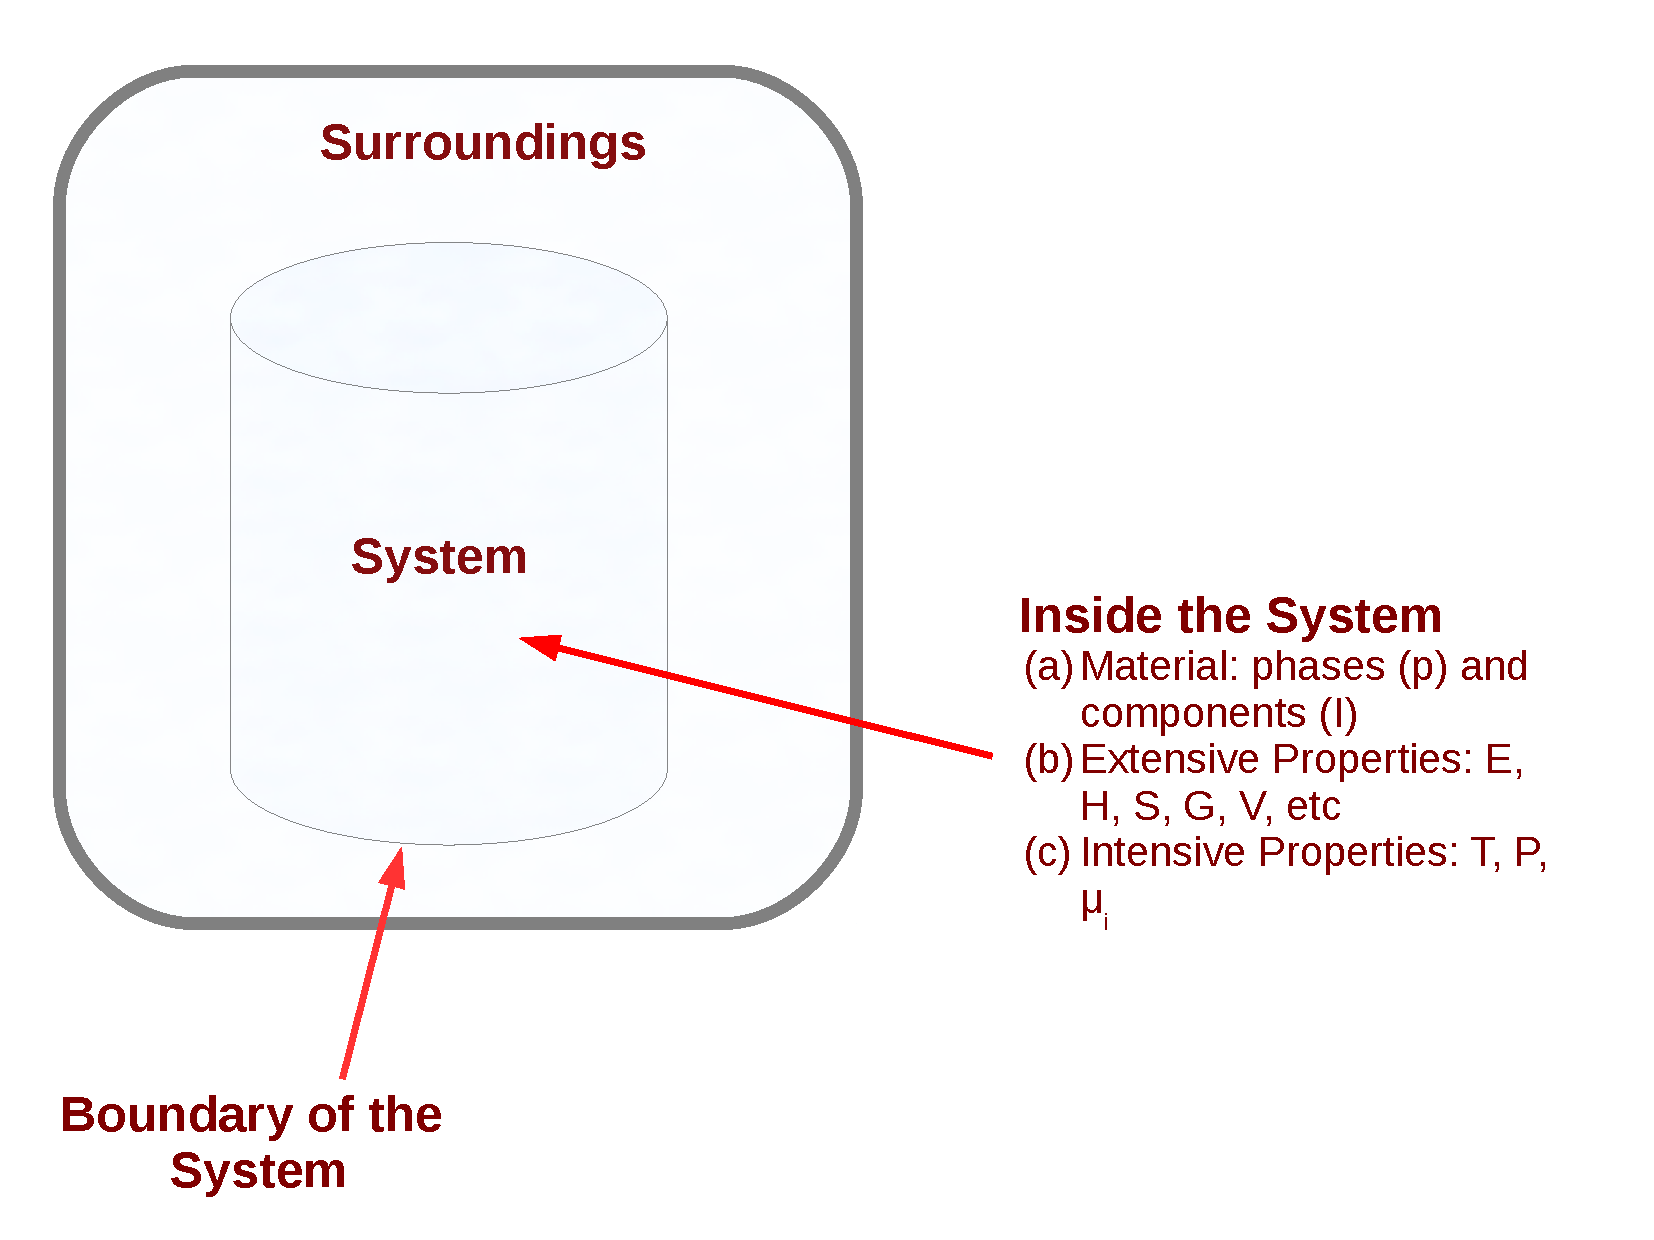
\includegraphics[width=1.05\columnwidth,clip]{./Pics/Fig_SystemDefinition}
        \end{center}
      \end{figure}
      \begin{tabular}{|c|c|c|}
         \hline
                      & {\bf Mass} & {\bf Energy} \\
                      & {\bf Exchange} & {\bf Exchange} \\
         \hline
         {\bf Open}   & {\it yes}  & {\it yes}    \\
         {\bf Closed} & {\it no}   & {\it yes}    \\
         {\bf Isolated}&{\it no}   & {\it no}     \\
         \hline 
      \end{tabular}    
    \end{column}
  \end{columns}
\end{frame}
\normalsize

%%%
%%% Slide
%%%
\scriptsize
\begin{frame}
 \frametitle{System and Control Volumes}
  \begin{columns}
    \begin{column}[l]{0.55\linewidth}
      \begin{itemize}%\scriptsize
       \item <1-> A \textcolor{red}{closed system} (also known as a \textcolor{red}{control mass}) consists of a fixed amount of mass, and no mass can cross its boundary. However, energy (in the form of heat or work) may cross the boundary -- and the volume of a closed system does not have to be fixed; 
       \item <2-> When neither energy nor mass is allowed to cross the boundary, that system is called an \textcolor{red}{isolated system};
       \item <3-> An \red{open system} (or \textcolor{red}{control volume}) is a properly selected region in space. It usually encloses a device that involves mass flow such as a compressor, turbine, or nozzle.
      \end{itemize}
    \end{column}
    \begin{column}[l]{0.45\linewidth}\scriptsize
      \begin{figure}%
        \begin{center}
          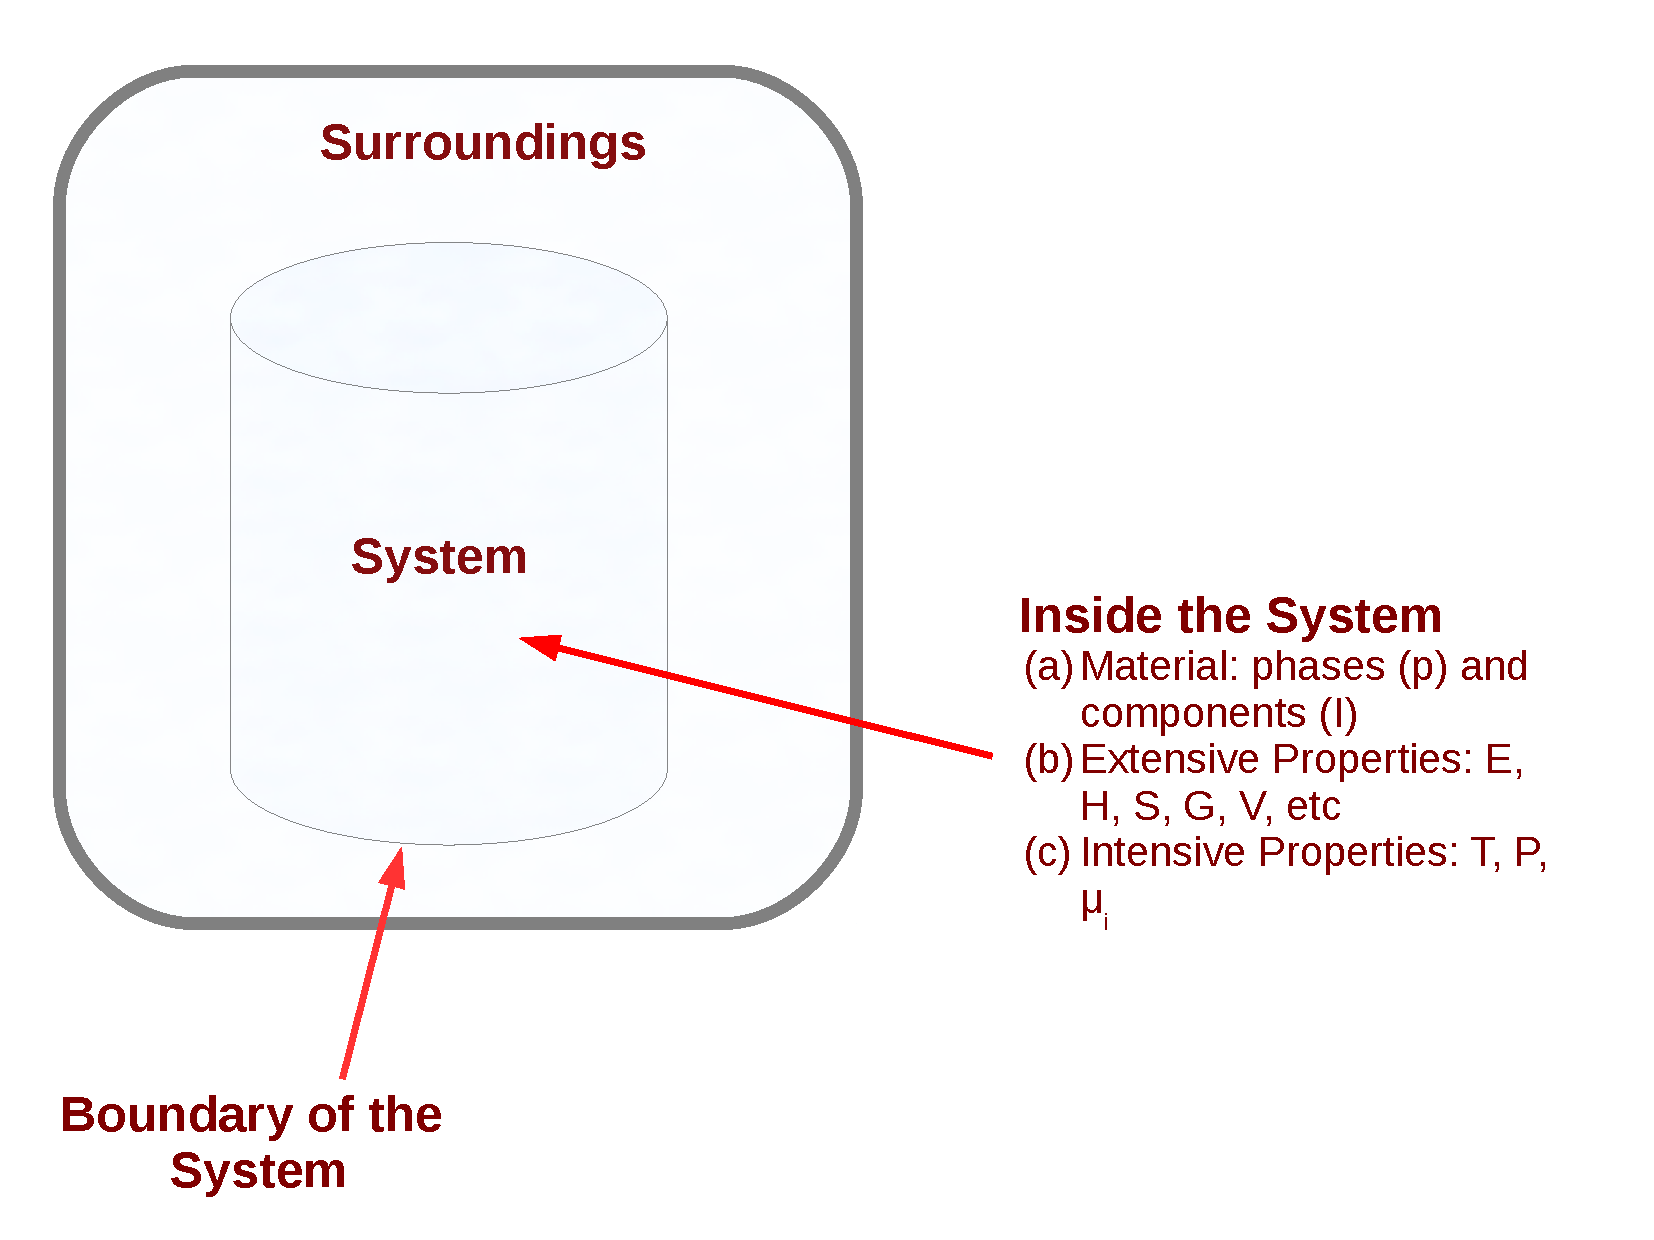
\includegraphics[width=1.05\columnwidth,clip]{./Pics/Fig_SystemDefinition}
        \end{center}
      \end{figure}
      \begin{tabular}{|c|c|c|}
         \hline
                      & {\bf Mass} & {\bf Energy} \\
                      & {\bf Exchange} & {\bf Exchange} \\
         \hline
         {\bf Open}   & {\it yes}  & {\it yes}    \\
         {\bf Closed} & {\it no}   & {\it yes}    \\
         {\bf Isolated}&{\it no}   & {\it no}     \\
         \hline 
      \end{tabular}    
    \end{column}
  \end{columns}
\end{frame}
\normalsize
\end{comment}

%%%
%%%
%%% Slide
%%%
\begin{frame}
 \frametitle{System and Control Volumes}
 \begin{itemize}
  \item <2-> The \textcolor{red}{material} in a system is composed of phases (e.g., solid, liquid, gas) with distinct physical and chemical properties;
  \item <3-> The \textcolor{red}{composition} of each phase is described by a series of discrete chemical formula units (i.e., chemical components) -- e.g., water/steam $\left(\right.$H$_{2}$O$\left.\right)$, ammonia $\left(\right.$NH$_{3}\left.\right)$, carbon dioxide $\left(\right.$CO$_{2}\left.\right)$, etc;
  \item <4-> Any characteristic of a system is called a \textcolor{red}{property} -- e.g., pressure, temperature, mass, etc;
  \item <5-> Properties can be classified as \textcolor{red}{intensive} or \textcolor{red}{extensive};
  \item <6-> \textcolor{red}{Intensive properties} are those that are {\bf independent} of the mass of a system -- e.g., temperature, pressure, density, viscosity, etc;
  \item <7-> \textcolor{red}{Extensive properties} are those whose values {\bf depend} on the size (or extent) of the system -- e.g., mass, volume, number of moles, internal energy, enthalpy, entropy, etc.  
 \end{itemize}
\end{frame}

\begin{comment}

\subsection{Review of the Main Thermodynamic Tools}
%%%
%%% Slide
%%%

\begin{frame}
 \frametitle{PVT Behaviour of Pure Substances}
 \begin{columns}
  \begin{column}[l]{0.5\linewidth}
\begin{itemize}
\item <1-> This surface represents the \textcolor{red}{Pressure} - \textcolor{red}{specific volume} - \textcolor{red}{Temperature} -- $PVT$, relation in a pure substance;
\item <2-> Any given coordinate in both, the surface plot and diagrams (projections), will represent values of pressure, specific volume and temperature when the substance is at equilibrium;
\end{itemize}
  \end{column}
  \begin{column}[l]{0.5\linewidth}
   \begin{figure}%
    \begin{center}
     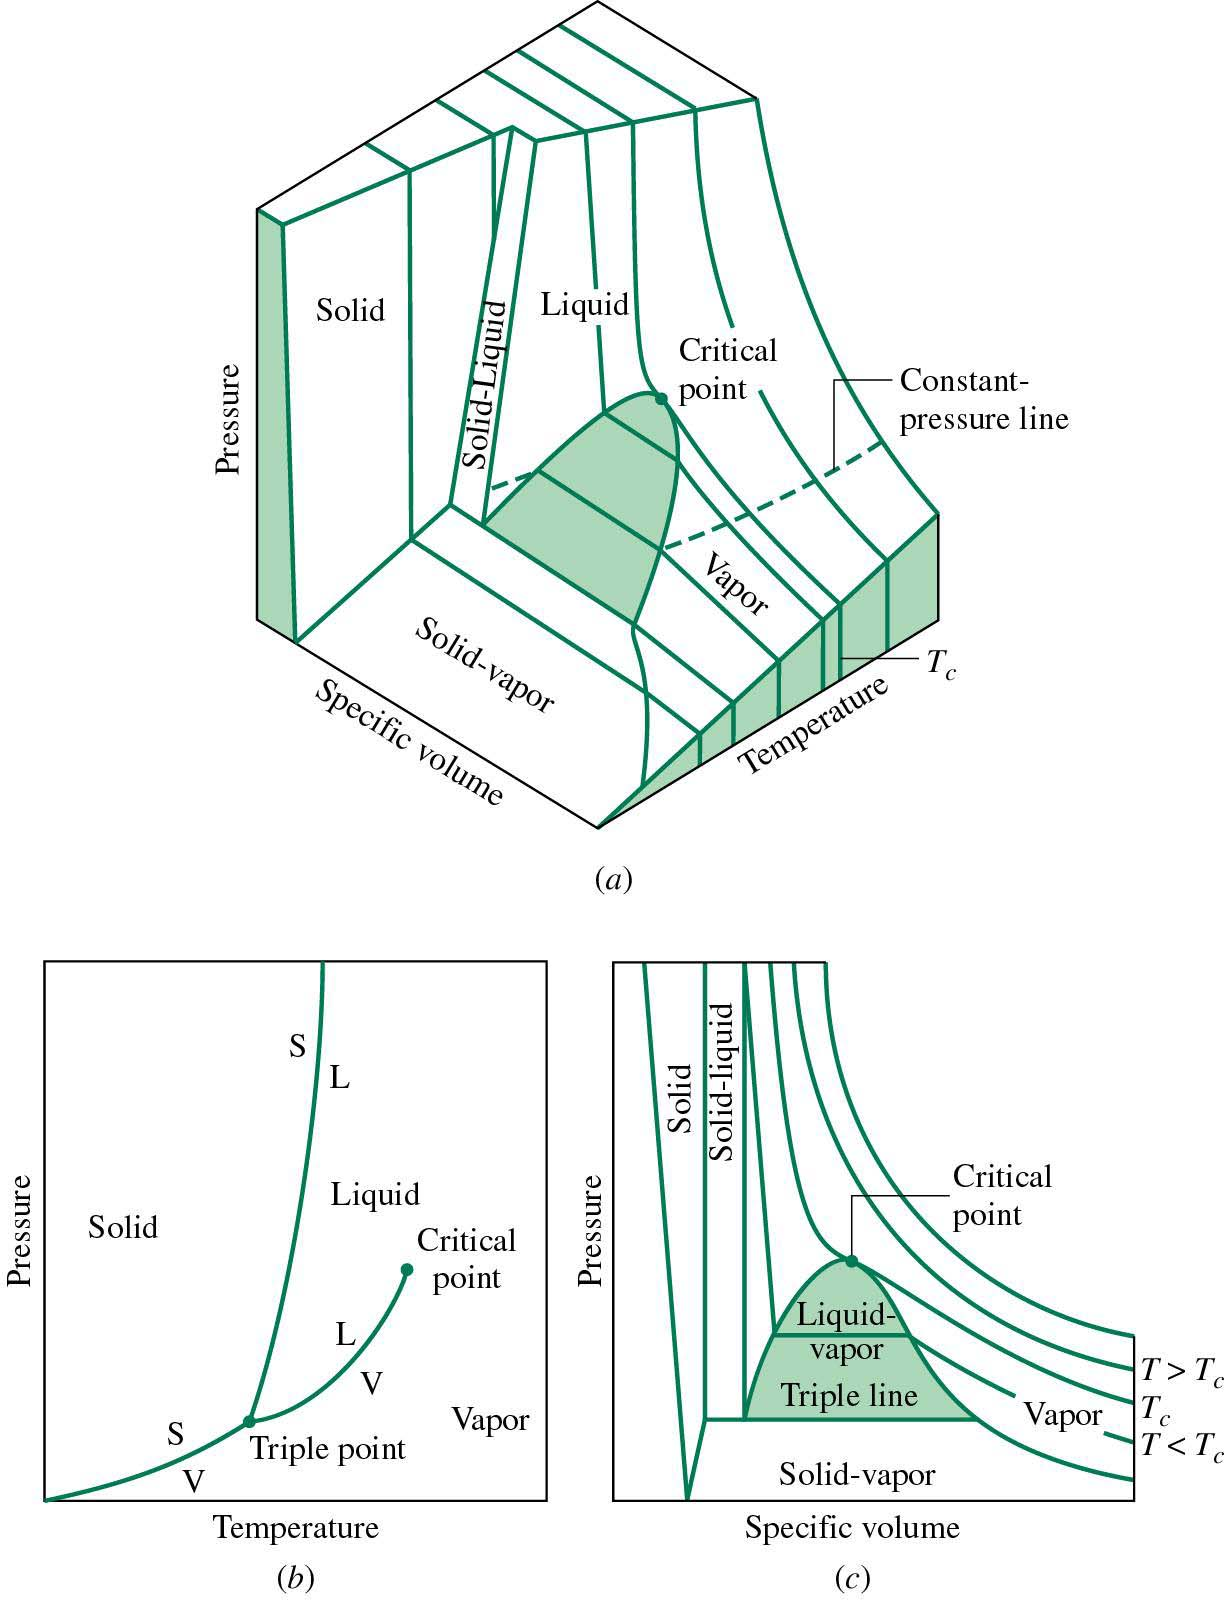
\includegraphics[width=4.cm,clip]{./Pics/PVT_Surface.jpg}
    \end{center}
\caption{$PVT$ surface (top) and projections onto (b) $PT$ and (c) $PV$ diagrams for a pure substance (Extracted from Moran {\it et al.})}
   \end{figure}    
  \end{column}
 \end{columns}
\end{frame}



%%%
%%% Slide
%%%

\begin{frame}
 \frametitle{PVT Behaviour of Pure Substances}
 \begin{columns}
  \begin{column}[l]{0.5\linewidth}
\begin{itemize}
\item <1-> The \textcolor{red}{Gibbs phase rule},
\begin{equation}
\Psi = 2 + \mathcal{C} - \mathcal{P}
\end{equation} 
\item <2-> describes the number of degrees of freedom (dof), $\Psi$ (intensive variables, e.g., temperature, pressure), in a closed system at equilibrium as a function of the number of phases ($\mathcal{P}$ = solid, liquid and vapour) and components, $\mathcal{C}$ (e.g., water, CO$_{2}$, N$_{2}$, etc). 
\end{itemize}
  \end{column}
  \begin{column}[l]{0.5\linewidth}
   \begin{figure}%
    \begin{center}
     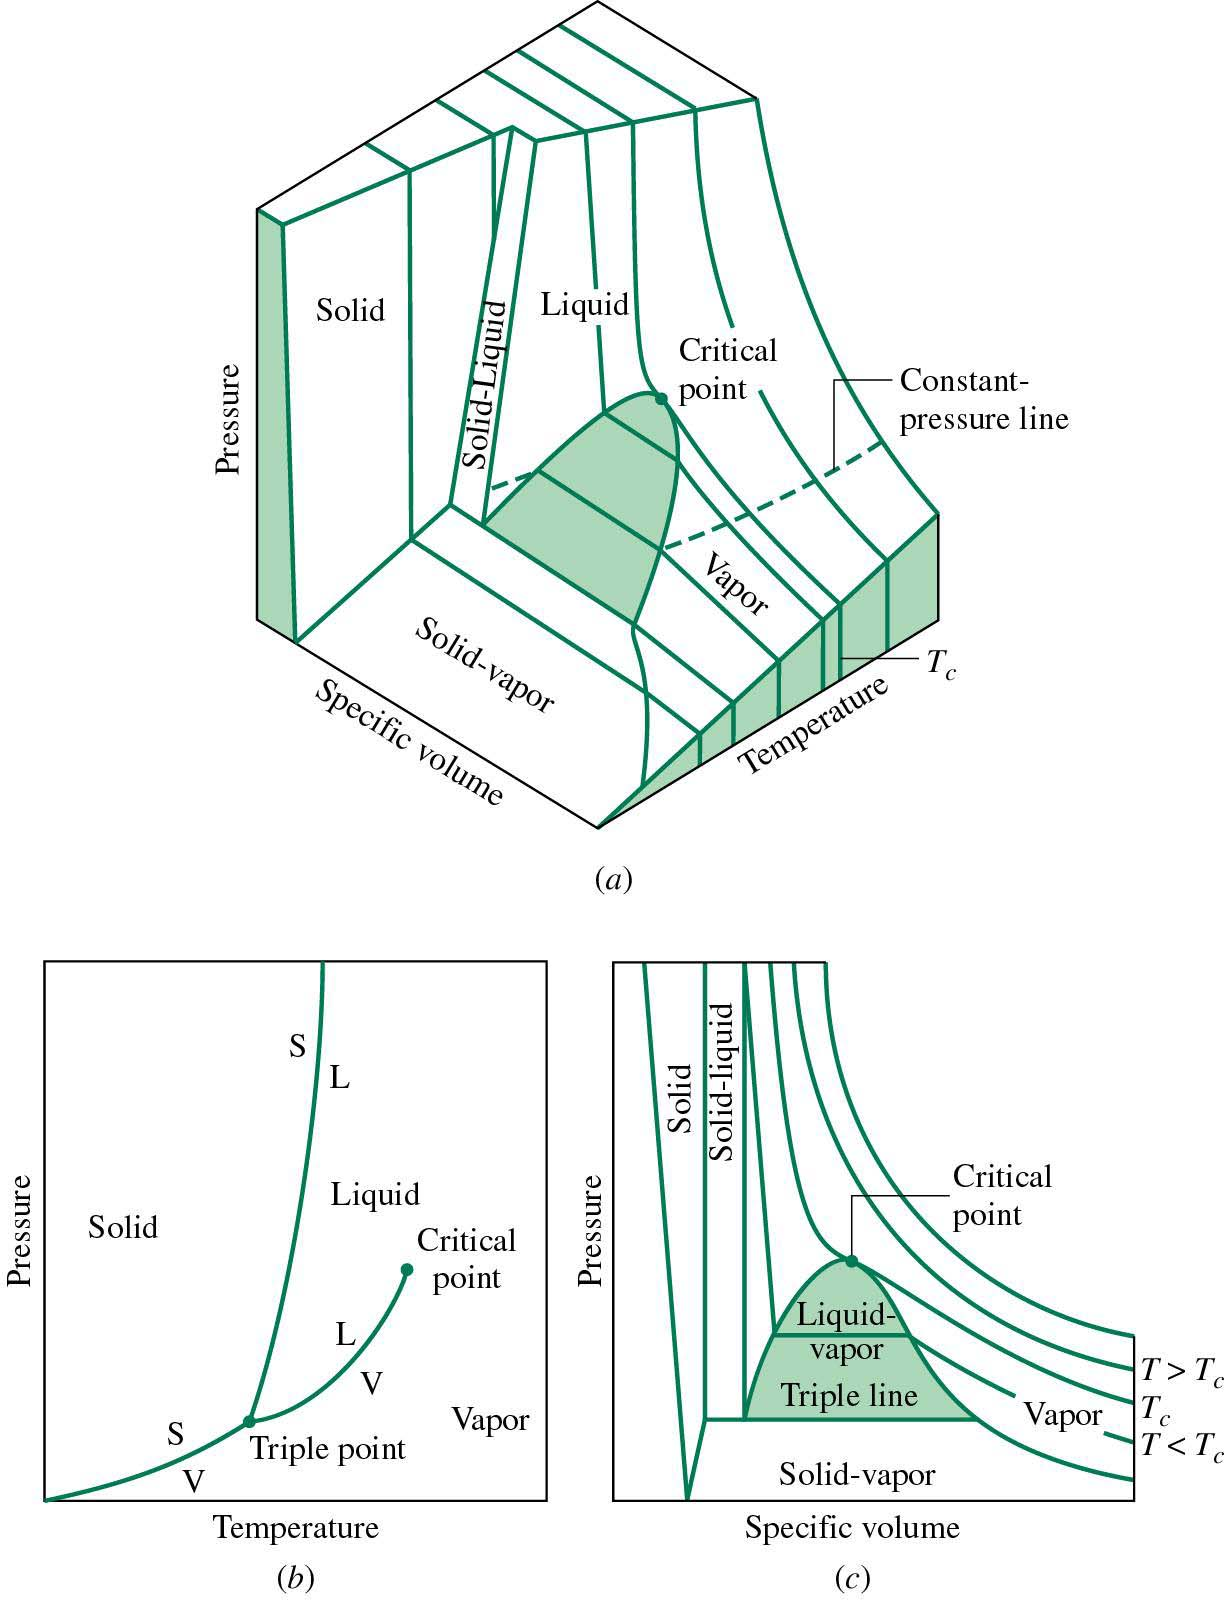
\includegraphics[width=4.cm,clip]{./Pics/PVT_Surface.jpg}
    \end{center}
\caption{$PVT$ surface (top) and projections onto (b) $PT$ and (c) $PV$ diagrams for a pure substance (Extracted from Moran {\it et al.})}
   \end{figure}    
  \end{column}
 \end{columns}
\end{frame}


%%%
%%% Slide
%%%

\begin{frame}
 \frametitle{PVT Behaviour of Pure Substances}
 \begin{columns}
  \begin{column}[l]{0.55\linewidth}
\begin{itemize}
\item <1-> {\bf Example:} In the $PT$ diagram (b) for one hypothetical component -- $\textcolor{red}{\mathcal{C}=1}$, within each phase region -- $\textcolor{blue}{\mathcal{P}=1}$ (i.e., as either solid, liquid or vapour phases),
\begin{displaymath}
\Psi = 2 + \textcolor{red}{1} - \textcolor{blue}{1} = 2
\end{displaymath}
\item <2-> In this case, the number of degrees of freedom correspond to temperature and pressure;
\item <3-> Thus, within (e.g.) the vapour phase, temperature and pressure can readily be changed without explicit phase change or composition of the vapour phase.
\end{itemize}
  \end{column}
  \begin{column}[l]{0.45\linewidth}
   \begin{figure}%
    \begin{center}
     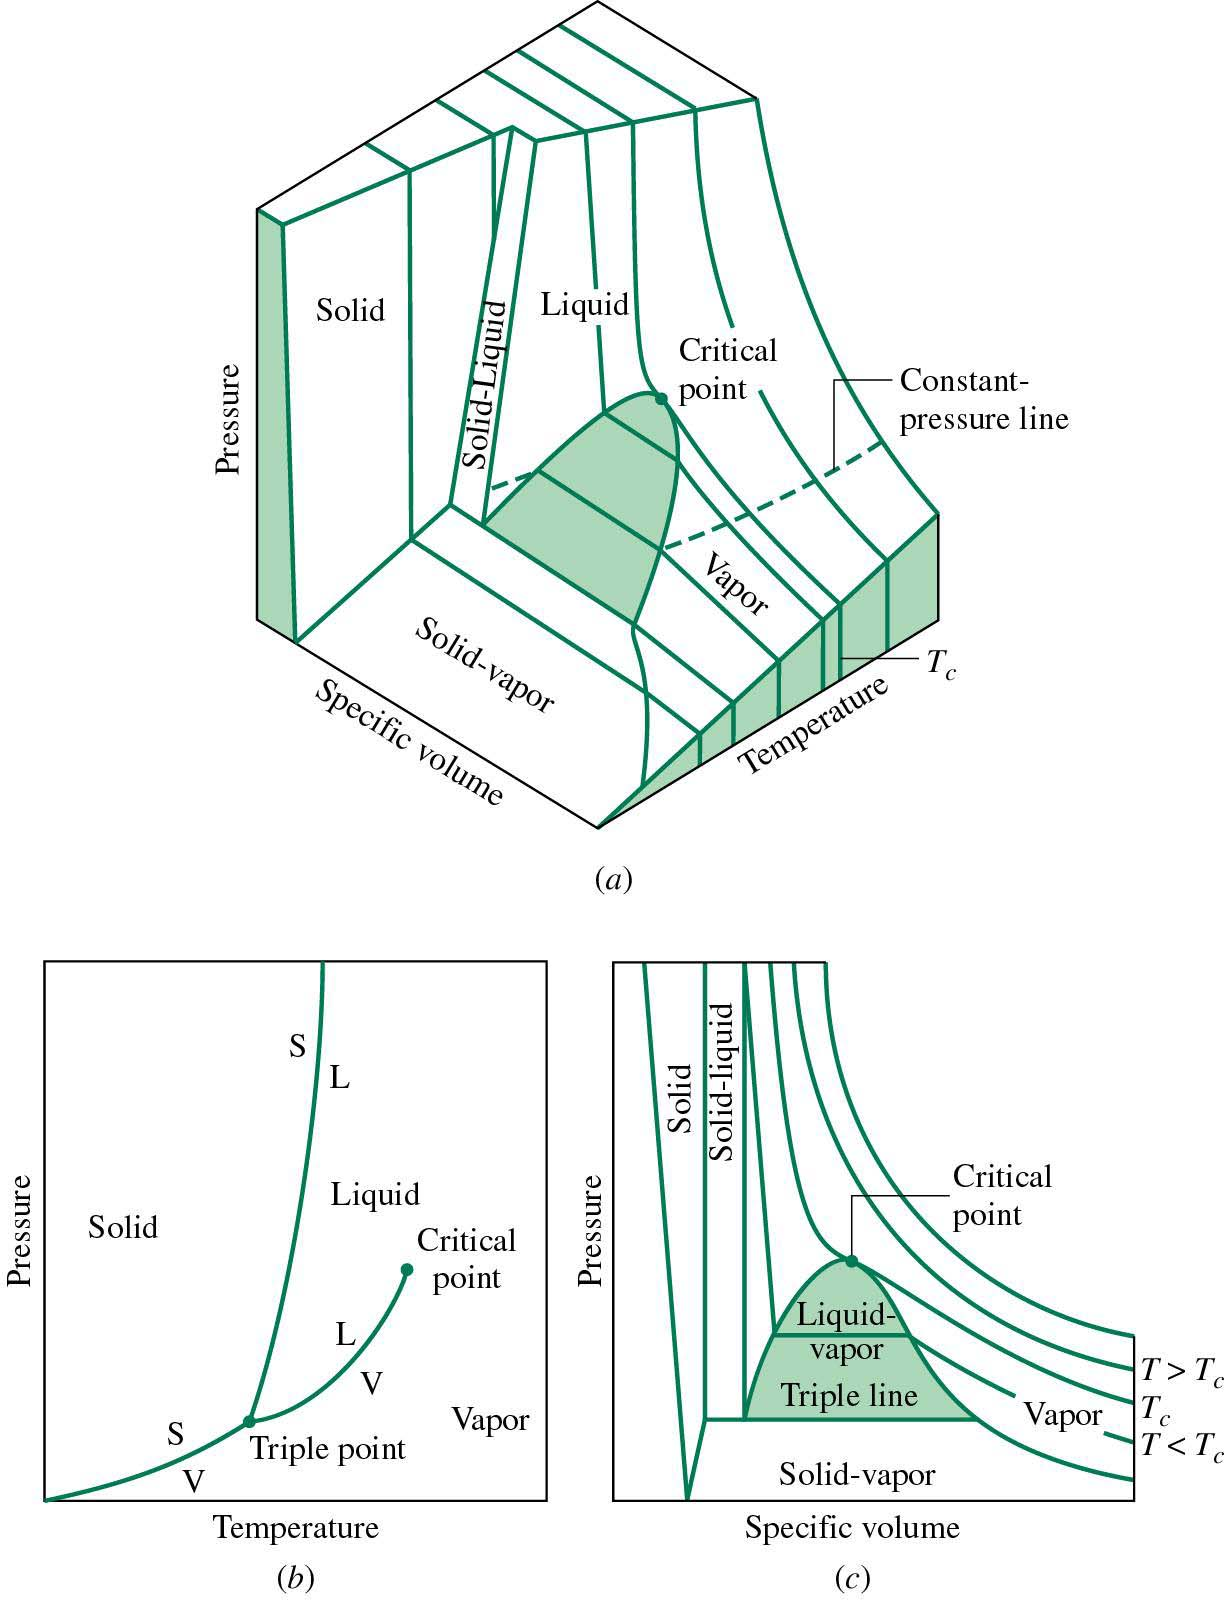
\includegraphics[width=4.cm,clip]{./Pics/PVT_Surface.jpg}
    \end{center}
\caption{$PVT$ surface (top) and projections onto (b) $PT$ and (c) $PV$ diagrams for a pure substance (Extracted from Moran {\it et al.})}
   \end{figure}    
  \end{column}
 \end{columns}
\end{frame}


%%%
%%% Slide
%%%

\begin{frame}
 \frametitle{PVT Behaviour of Pure Substances}
 \begin{columns}
  \begin{column}[l]{0.5\linewidth}
\begin{itemize}
\item <1-> However, along with the \textcolor{red}{phase-line boundary}, two phases are in equilibrium, i.e., $\textcolor{blue}{\mathcal{P}=2}$,%
\begin{displaymath}
\Psi = 2 + \textcolor{red}{1} - \textcolor{blue}{2} = 1
\end{displaymath}
\item <2-> When the vapour and liquid phases are in equilibrium, any change in temperature {\bf leads} to change in pressure for the system remains in equilibrium;
\end{itemize}
  \end{column}
  \begin{column}[l]{0.5\linewidth}
   \begin{figure}%
    \begin{center}
     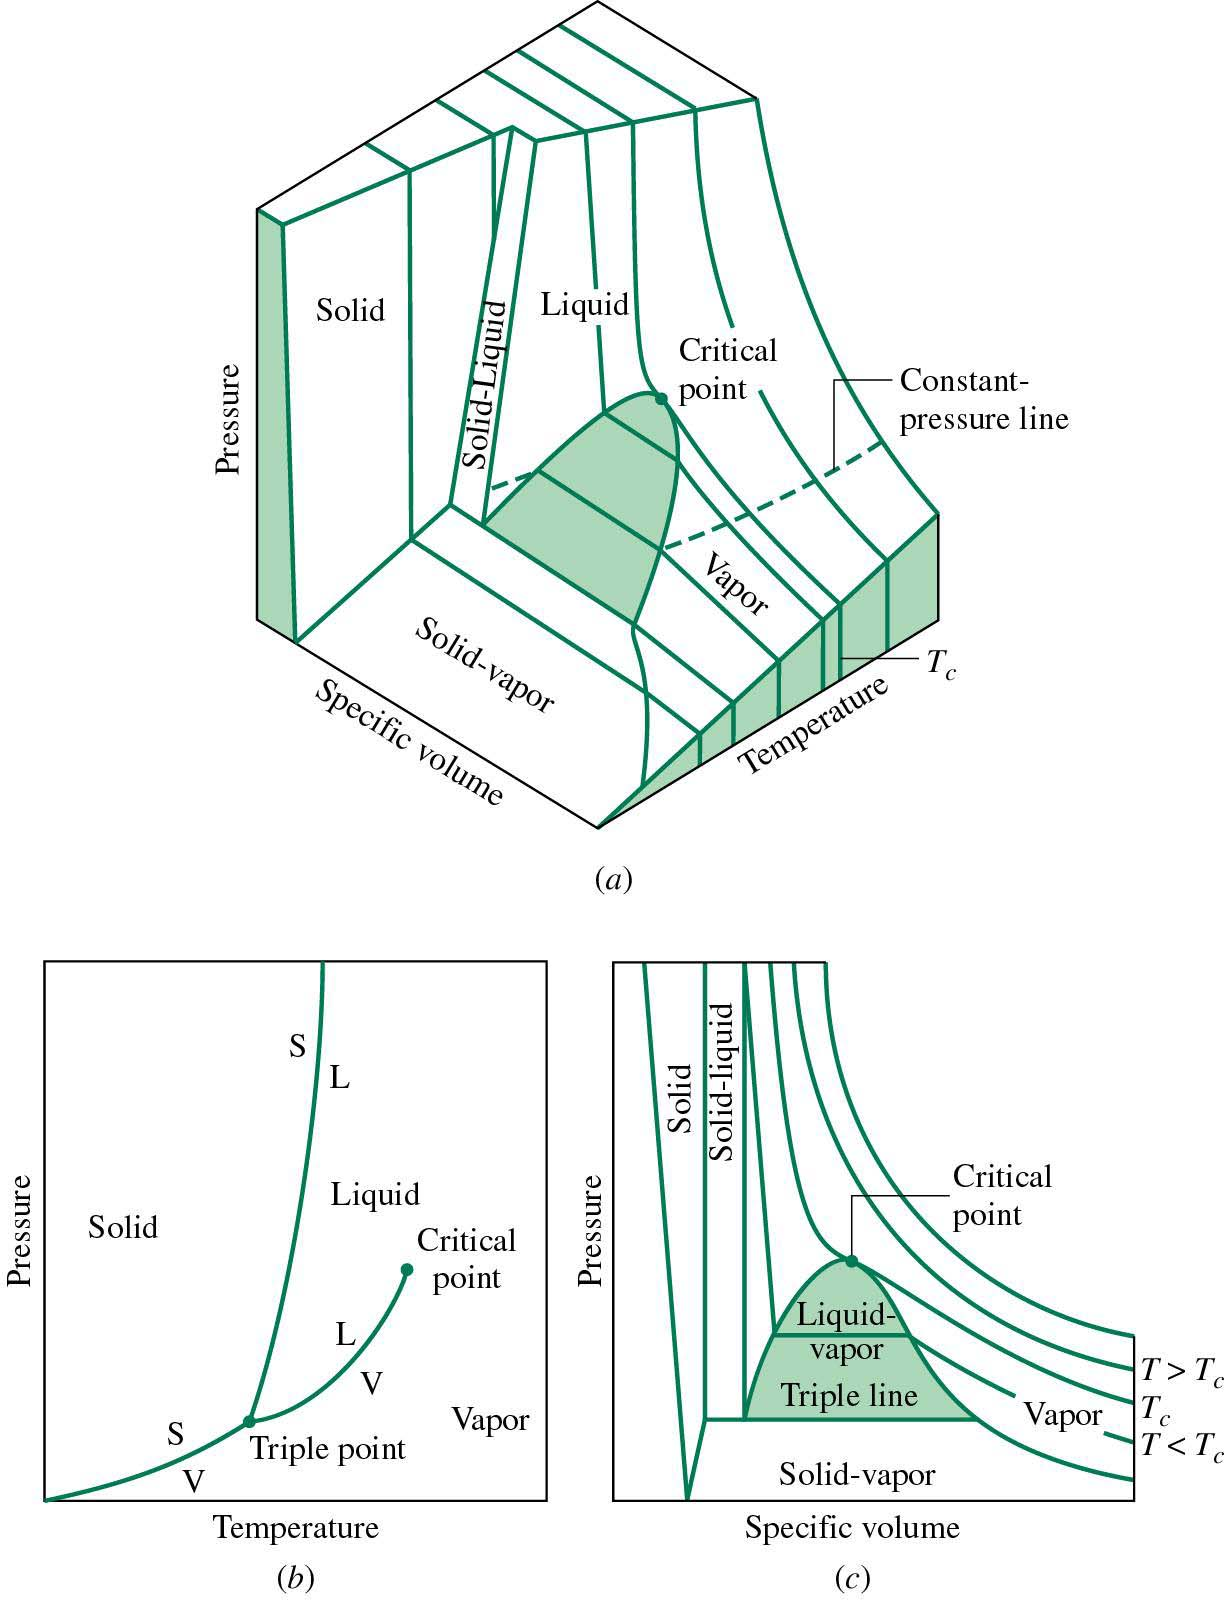
\includegraphics[width=4.cm,clip]{./Pics/PVT_Surface.jpg}
    \end{center}
\caption{$PVT$ surface (top) and projections onto (b) $PT$ and (c) $PV$ diagrams for a pure substance (Extracted from Moran {\it et al.})}
   \end{figure}    
  \end{column}
 \end{columns}
\end{frame}


%%%
%%% Slide
%%%

\begin{frame}
 \frametitle{PVT Behaviour of Pure Substances}
 \begin{columns}
  \begin{column}[l]{0.5\linewidth}
\begin{itemize}
\item <1-> Similarly, for the {\bf triple point} -- $\textcolor{blue}{\mathcal{P}=3}$, all three phases are in equilibrium
\begin{displaymath}
\Psi = 2 + \textcolor{red}{1} - \textcolor{blue}{3} = 0
\end{displaymath}
\item <2-> Here there is {\bf no degrees of freedom} -- i.e., there is {\bf just} one value for pressure and temperature that make the {\bf three phases to coexist}.
\item <3-> Any change in either intensive properties will drive the system away from the {\it triple point}.
\end{itemize}
  \end{column}
  \begin{column}[l]{0.5\linewidth}
   \begin{figure}%
    \begin{center}
     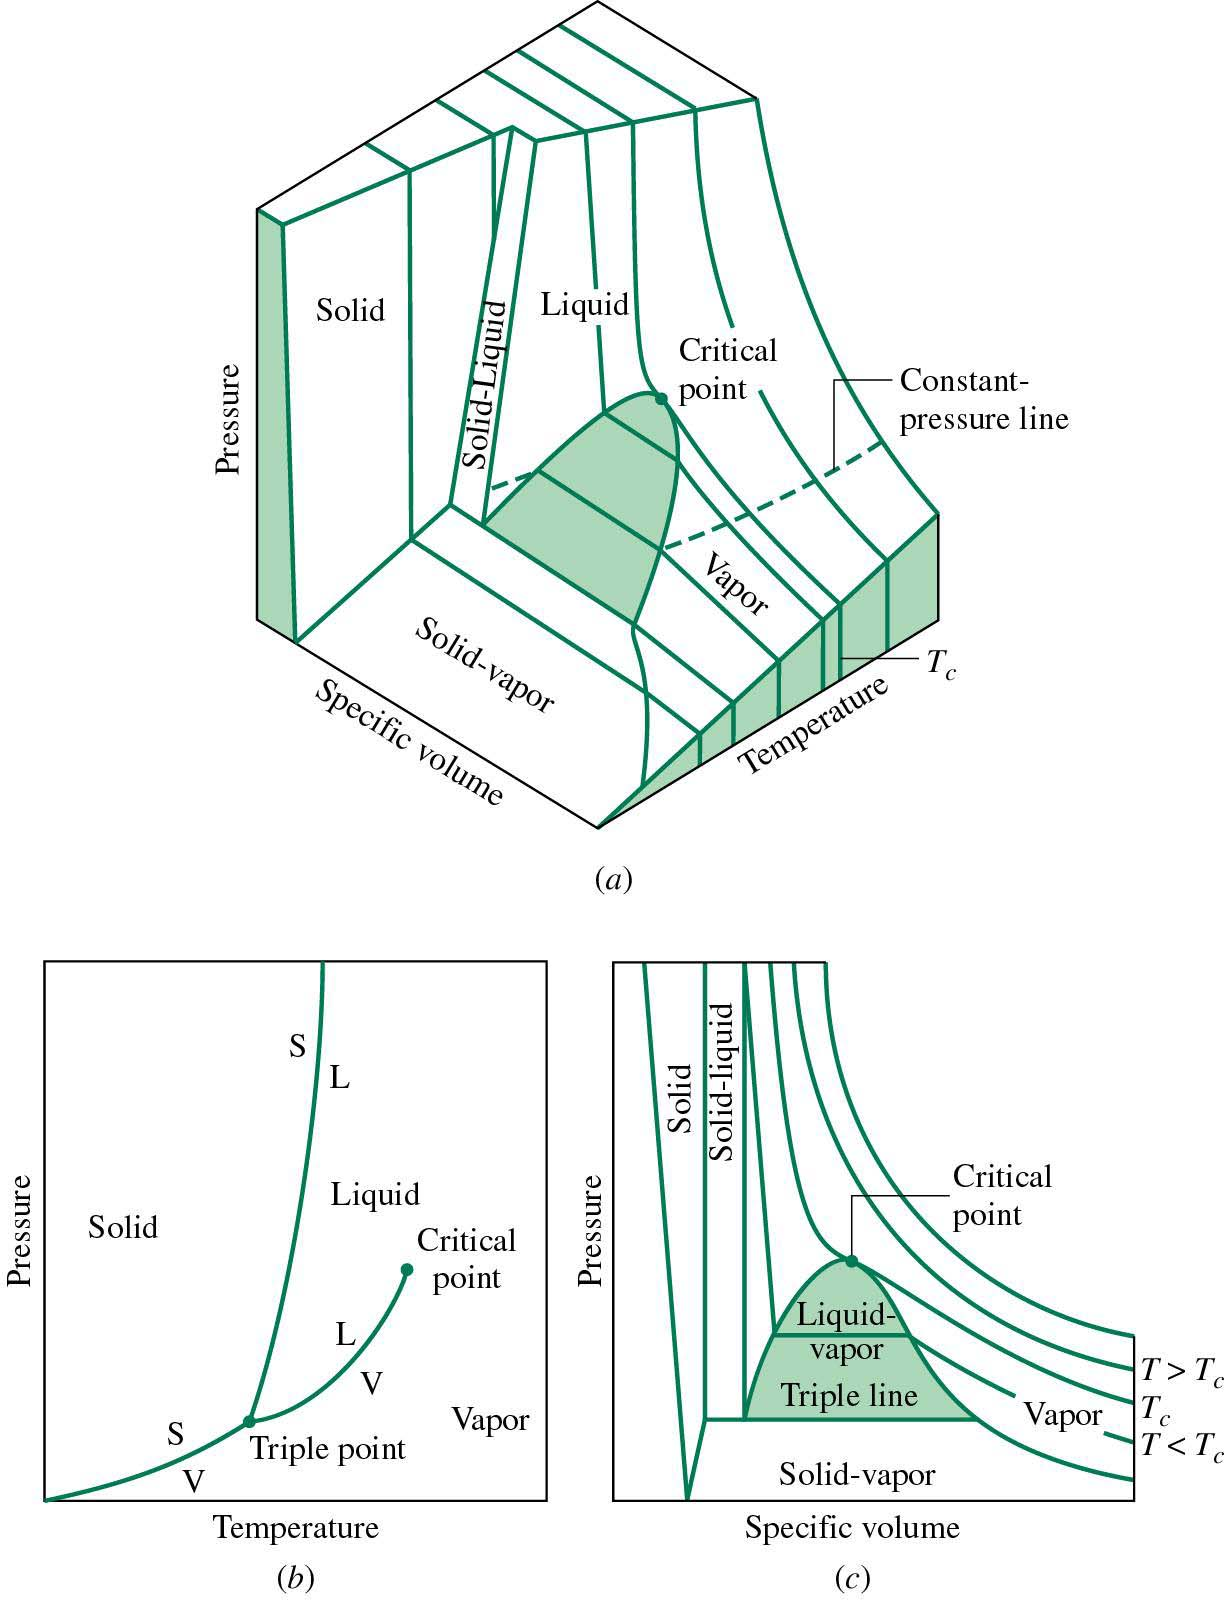
\includegraphics[width=4.cm,clip]{./Pics/PVT_Surface.jpg}
    \end{center}
\caption{$PVT$ surface (top) and projections onto (b) $PT$ and (c) $PV$ diagrams for a pure substance (Extracted from Moran {\it et al.})}
   \end{figure}    
  \end{column}
 \end{columns}
\end{frame}


\end{comment}
%%%
%%% SUBSECTION
%%%
\subsection{Thermodynamic Diagrams and Tables}

%%%
%%% Slide
%%%
\begin{frame}
 \frametitle{$PvT$ Thermodynamics Diagrams and Projected Surfaces}
  \begin{center}
   \begin{figure}
     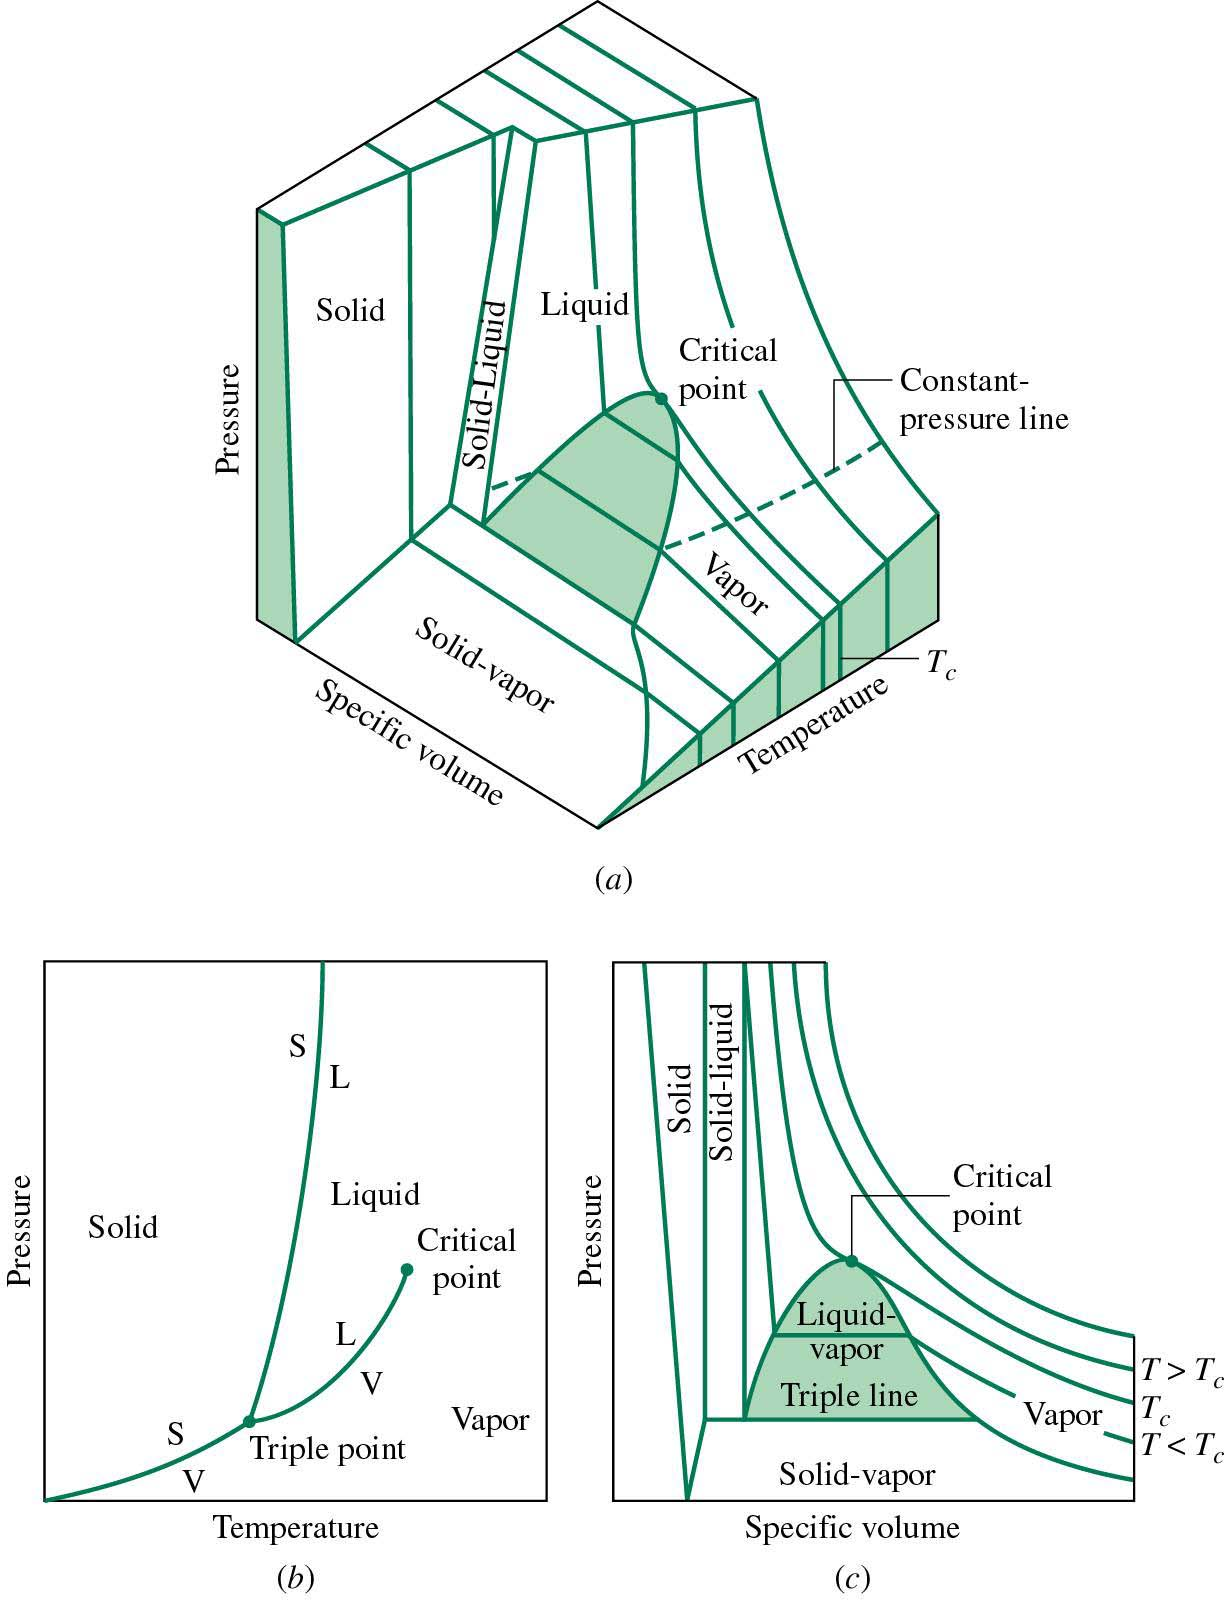
\includegraphics[width=8cm,height=6.cm,clip]{./Pics/PVT_Surface.jpg}
\caption{$PVT$ diagram (top) and projections onto (b) $PT$ and (c) $PV$ diagrams for a pure substance (Extracted from Moran {\it et al.}).}
   \end{figure}
   \end{center}
\end{frame}
%%%
%%% Slide
%%%
\begin{frame}
 \frametitle{Thermodynamics Diagrams: Pressure $\times$ Enthalpy $(PH)$ for CO$_{2}$}
  \begin{center}
   \begin{figure}
     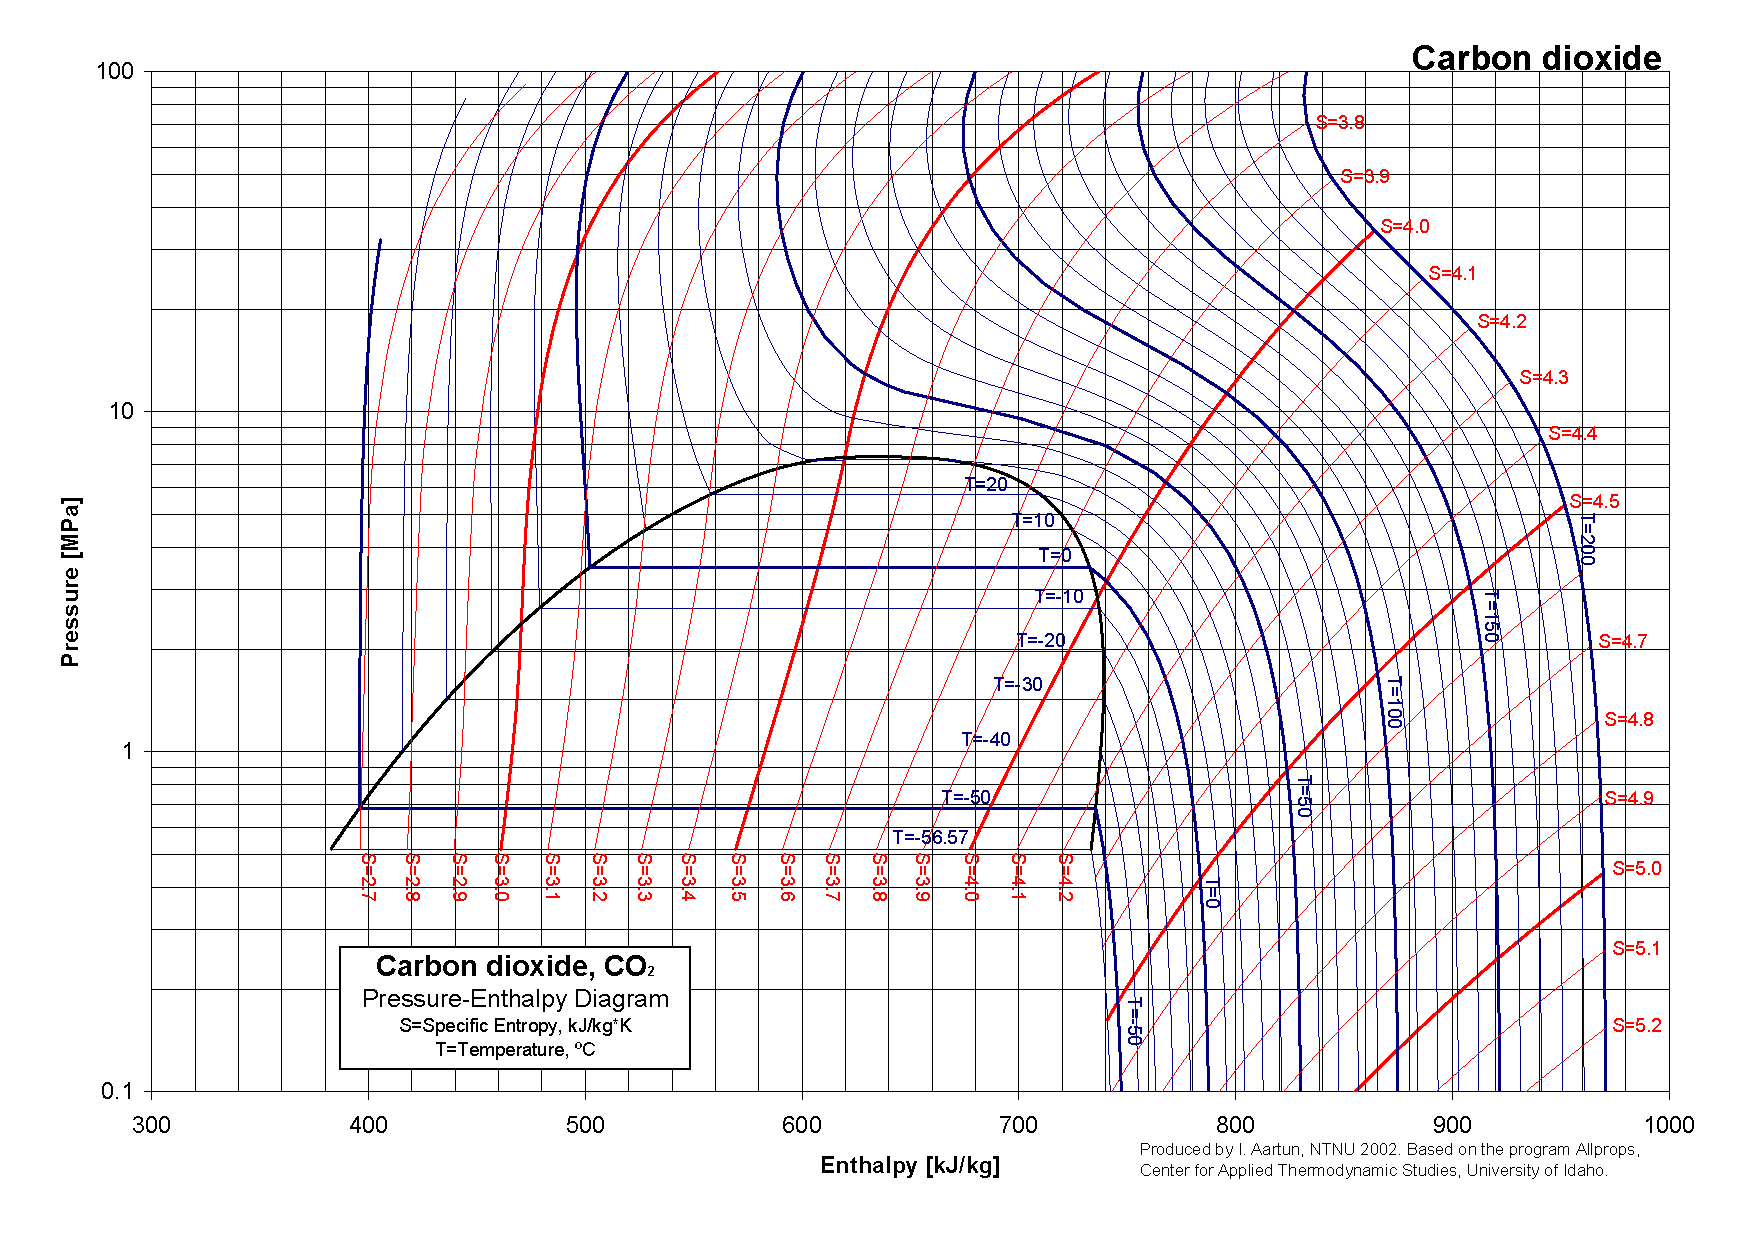
\includegraphics[width=8cm,height=7.cm,clip]{./Pics/CO2col}
   \end{figure}
   \end{center}
\end{frame}

%%%
%%% Slide
%%%
\begin{frame}
 \frametitle{Thermodynamics Diagrams: Pressure $\times$ Enthalpy $(PH)$}
  \begin{center}
   \begin{figure}
      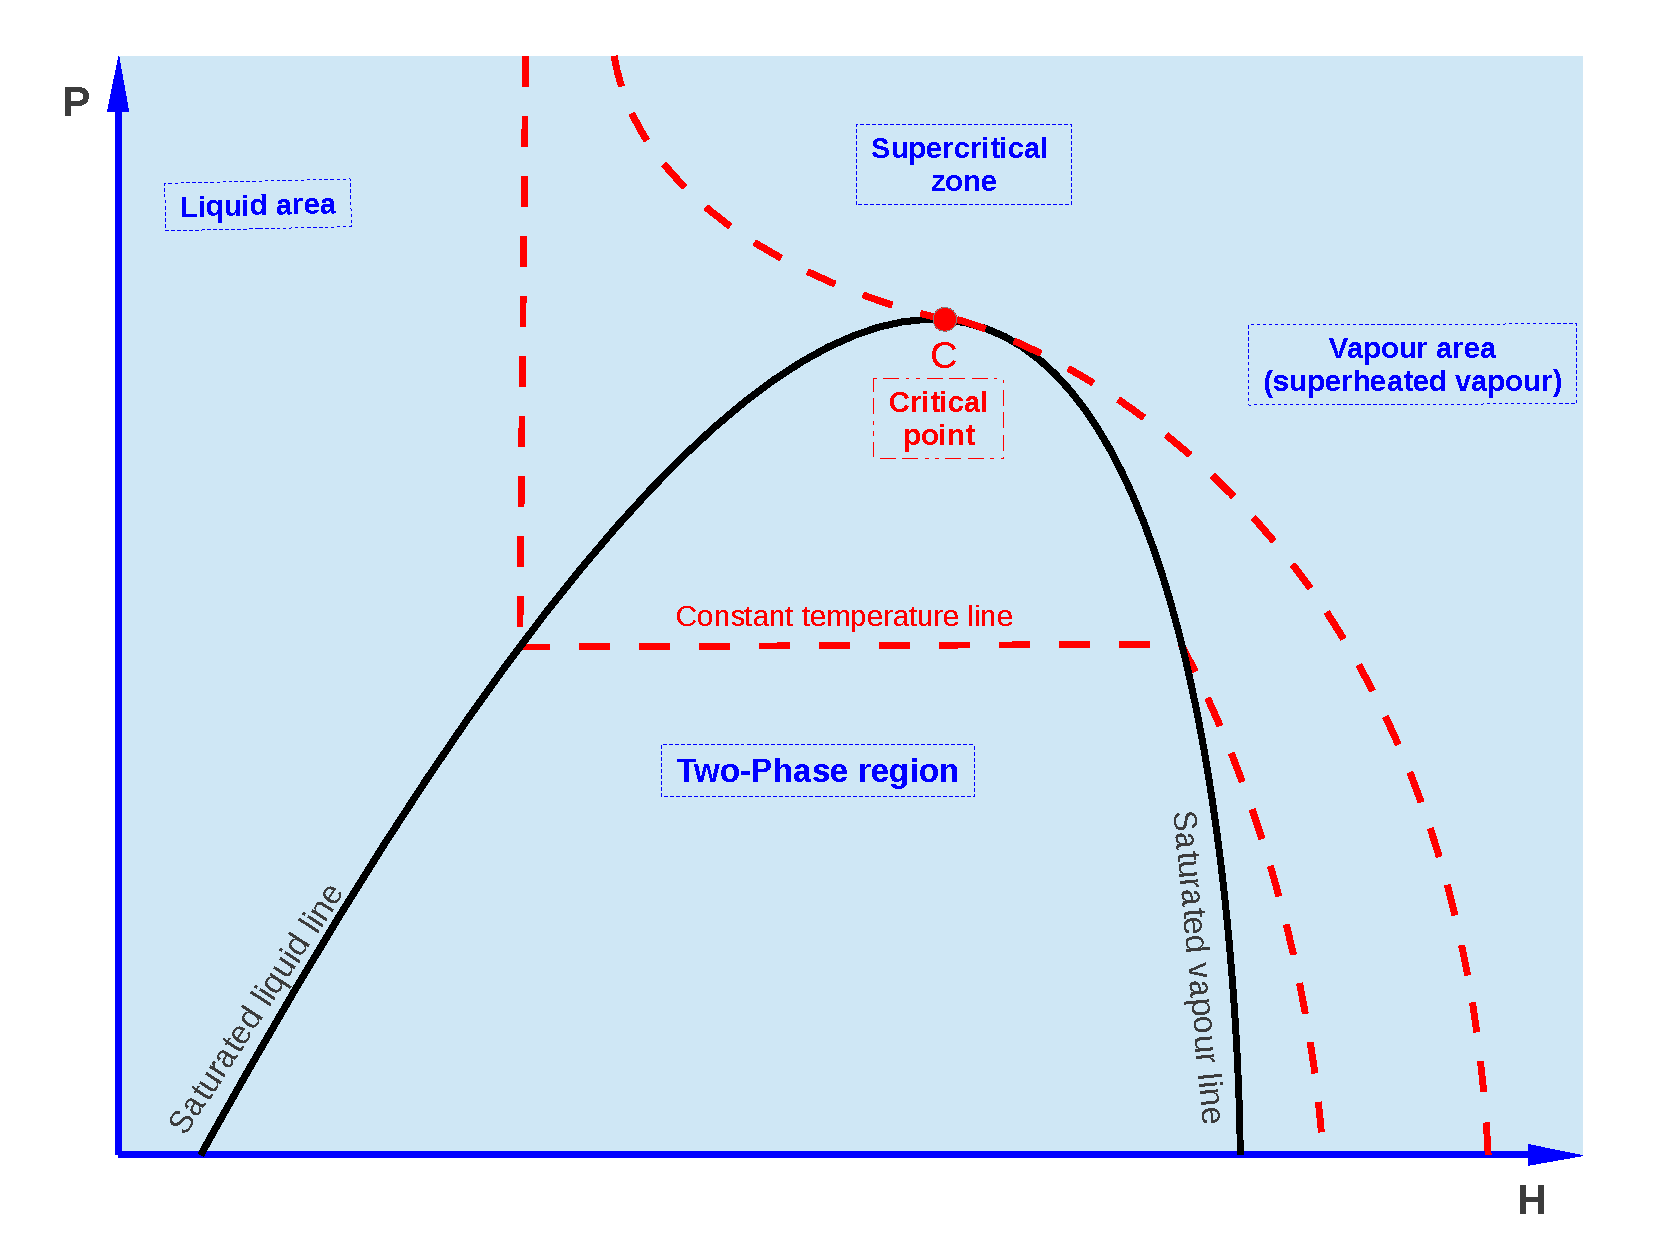
\includegraphics[width=8cm,height=7.9cm,clip]{./Pics/Overview_Refrig18}
   \end{figure}
   \end{center}
\end{frame}

%%%
%%% Slide
%%%
\begin{frame}
 \frametitle{Thermodynamics Diagrams: Pressure $\times$ Enthalpy $(PH)$}
  \begin{center}
   \begin{figure} 
      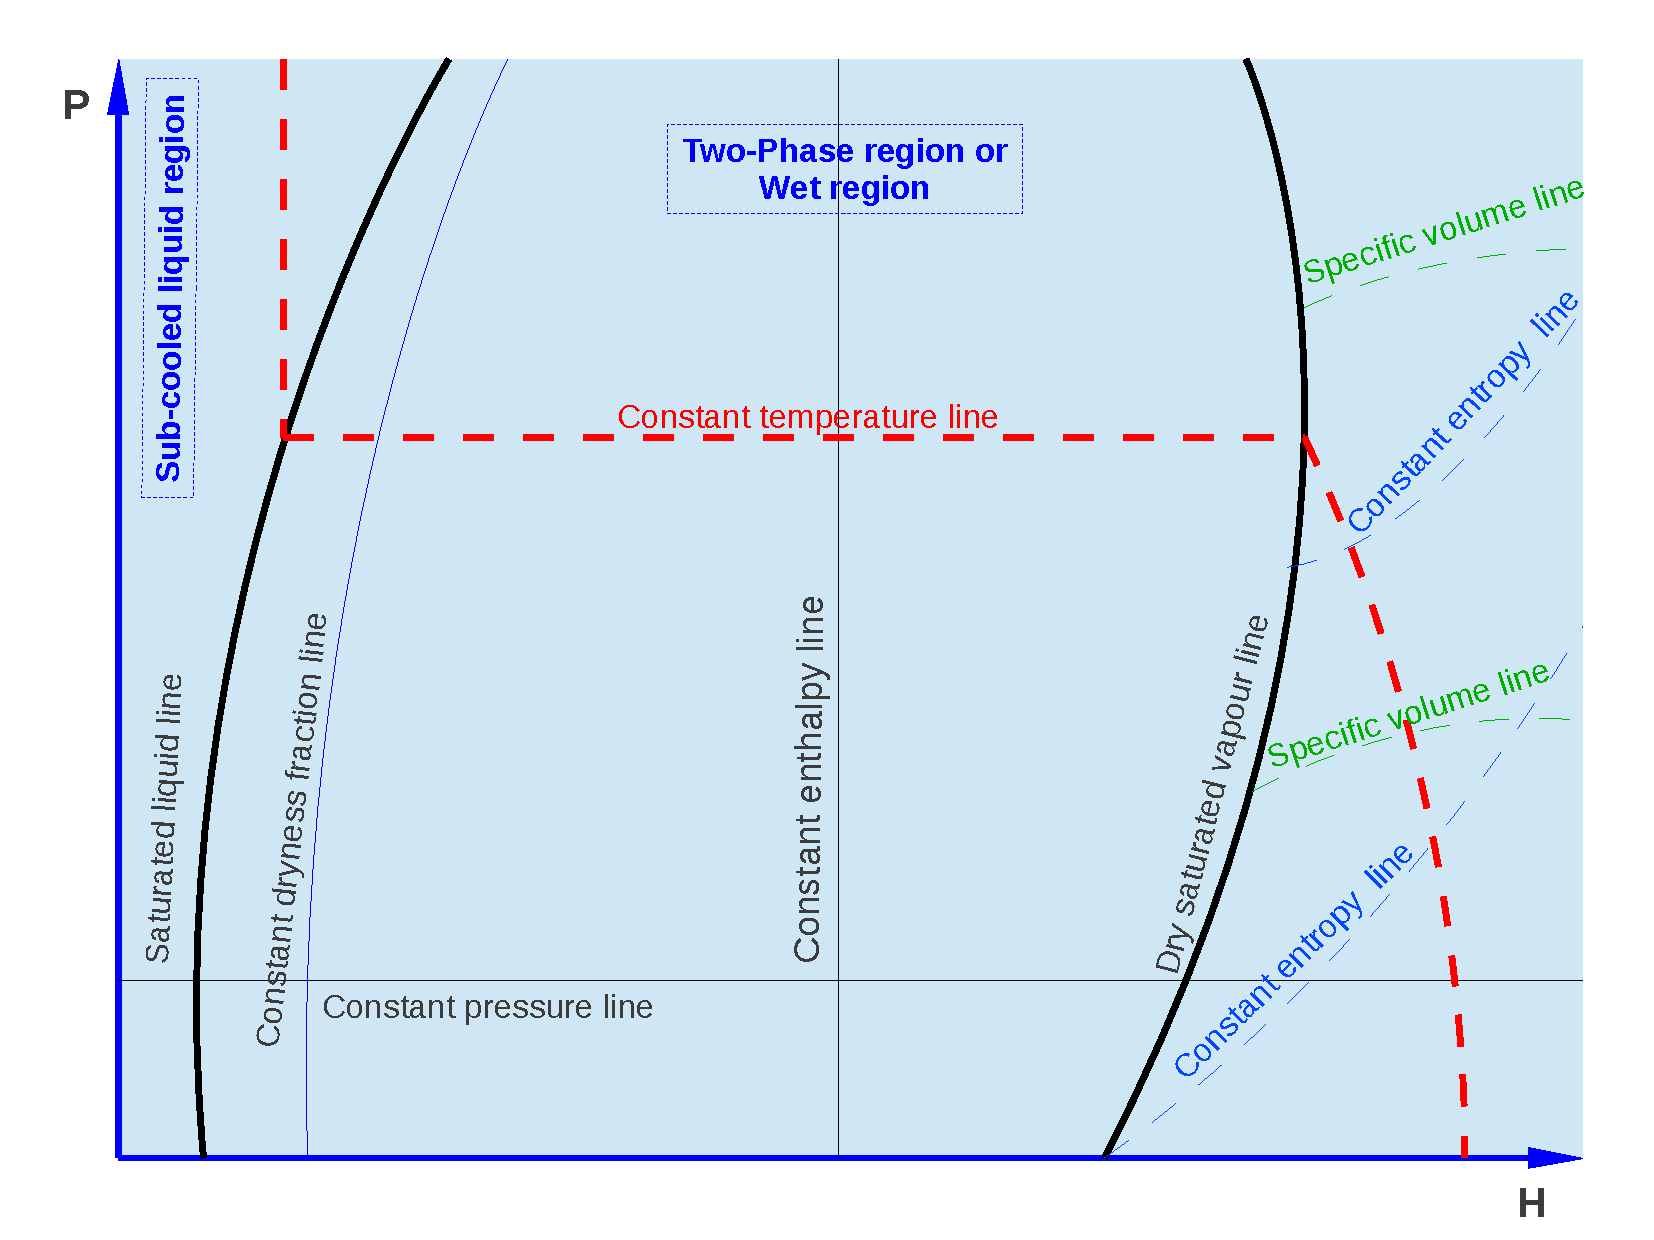
\includegraphics[width=8cm,height=7.9cm,clip]{./Pics/Overview_Refrig17}
   \end{figure}
   \end{center}
\end{frame}

%%%
%%% Slide
%%%
\begin{frame}
 \frametitle{Thermodynamics Diagrams: Temperature $\times$ Entropy $(TS)$ for Water}
  \begin{center}
   \begin{figure}
     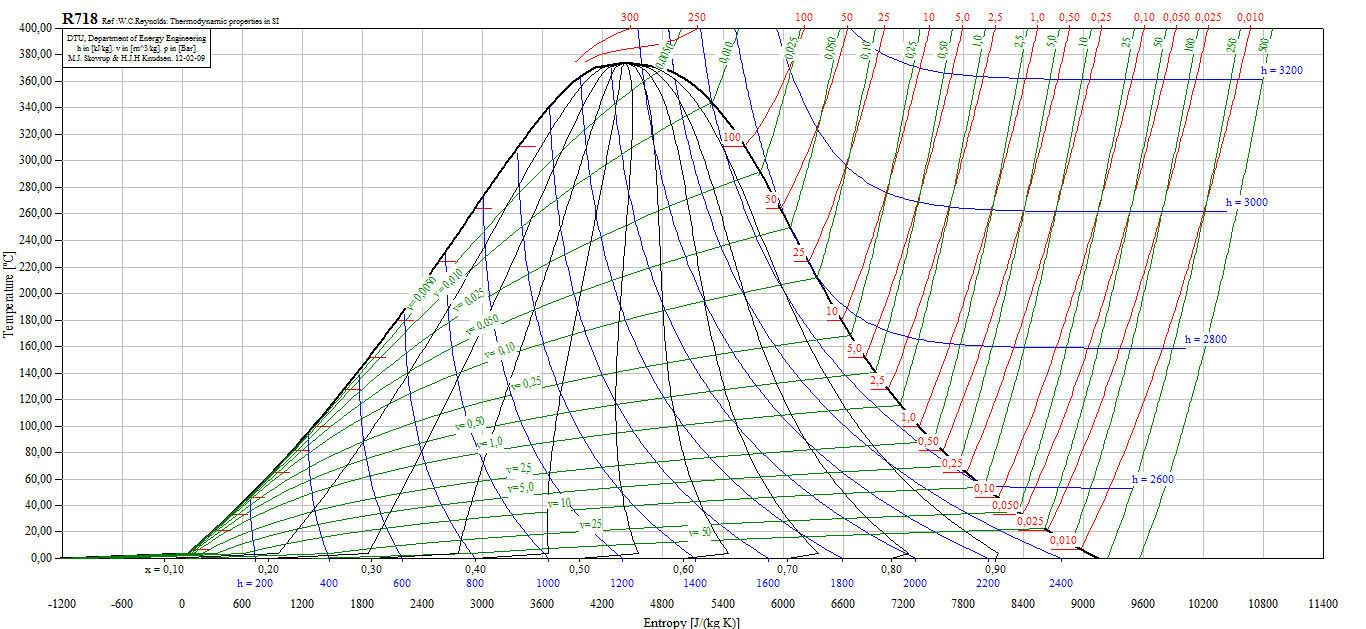
\includegraphics[width=8cm,height=7.cm,clip]{./Pics/water_TS.png}
   \end{figure}
   \end{center}
\end{frame}

%%%
%%% Slide
%%%
\begin{frame}
 \frametitle{Thermodynamics Diagrams: Temperature $\times$ Entropy $(TS)$}
  \begin{center}
   \begin{figure}
      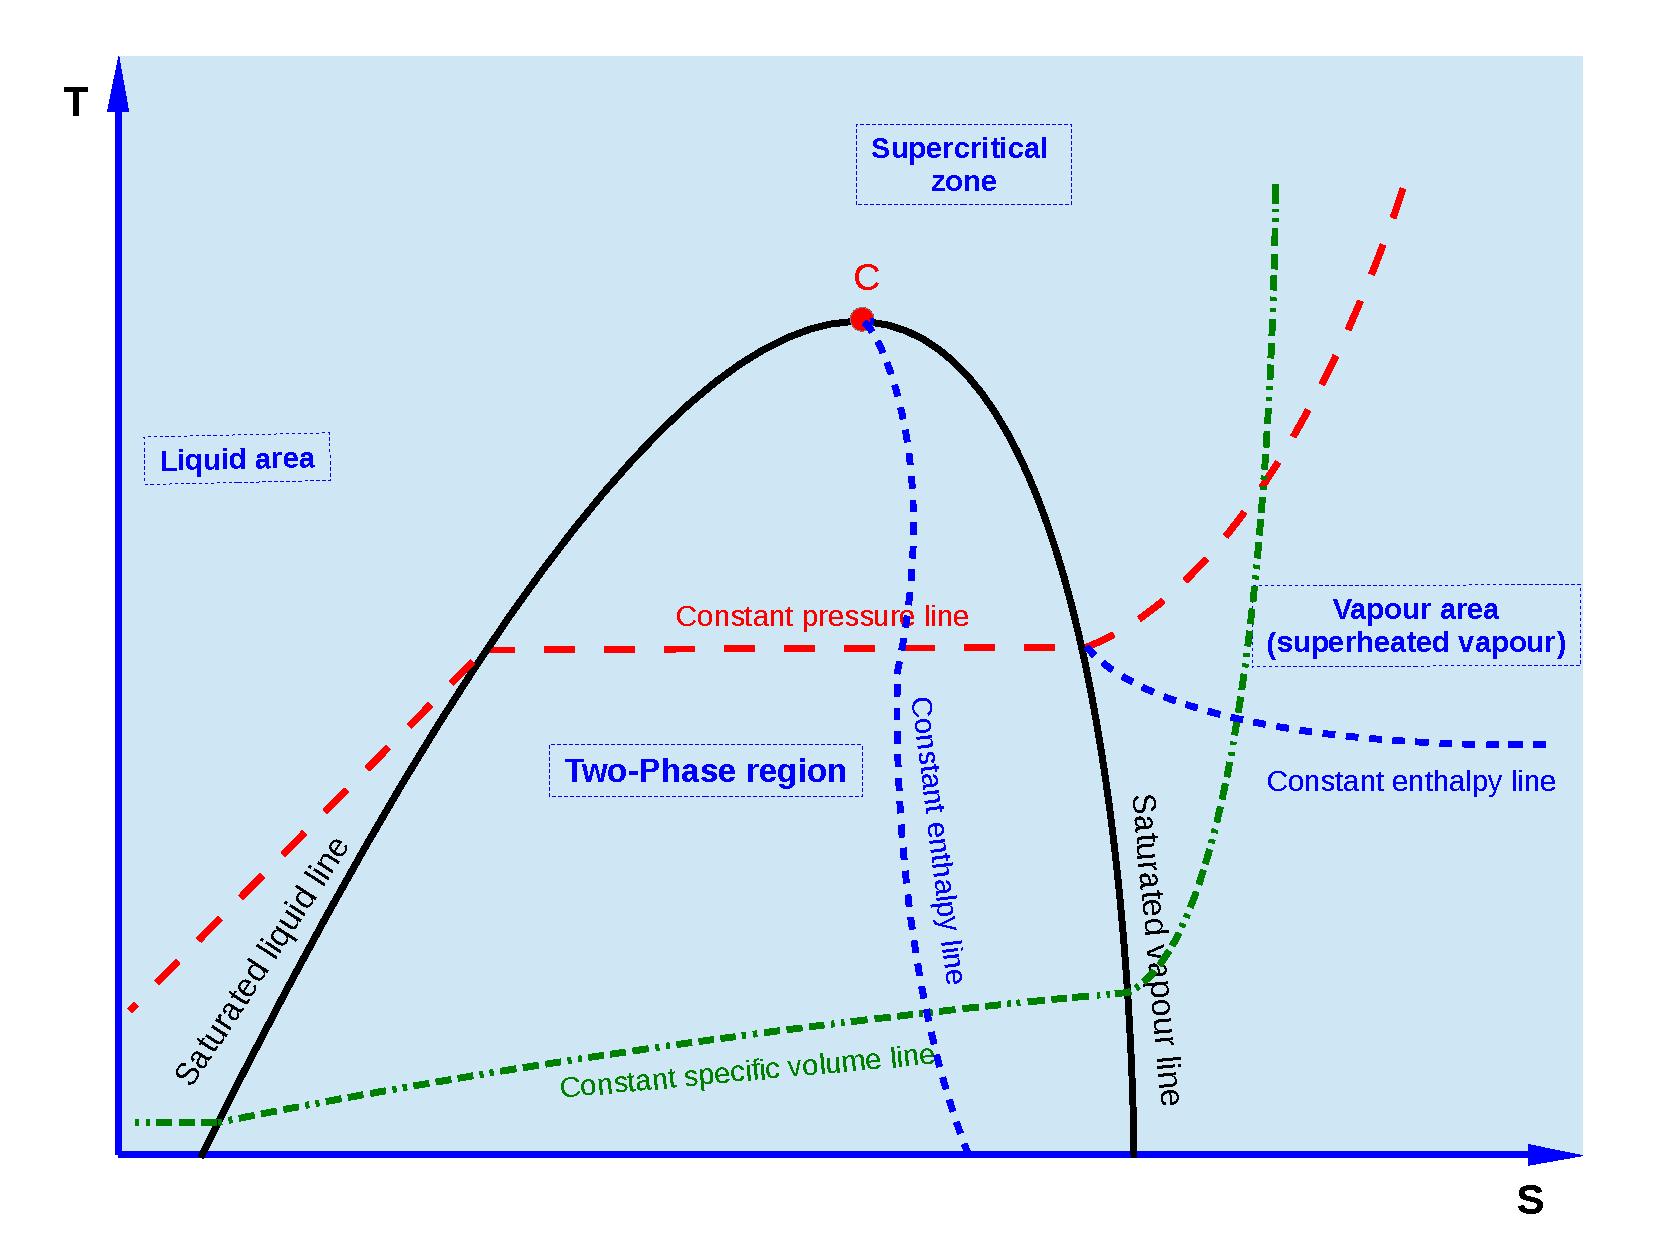
\includegraphics[width=8cm,height=7.9cm,clip]{./Pics/TS_Diag_Schematics}
   \end{figure}
   \end{center}
\end{frame}

%%% 
%%% Slide
%%%
\begin{frame}
  \frametitle{Another option: (a) Saturated Tables and ...}
\scriptsize{From Reference (d):}\vspace{-.8cm}
   \begin{center}
   \begin{figure}
      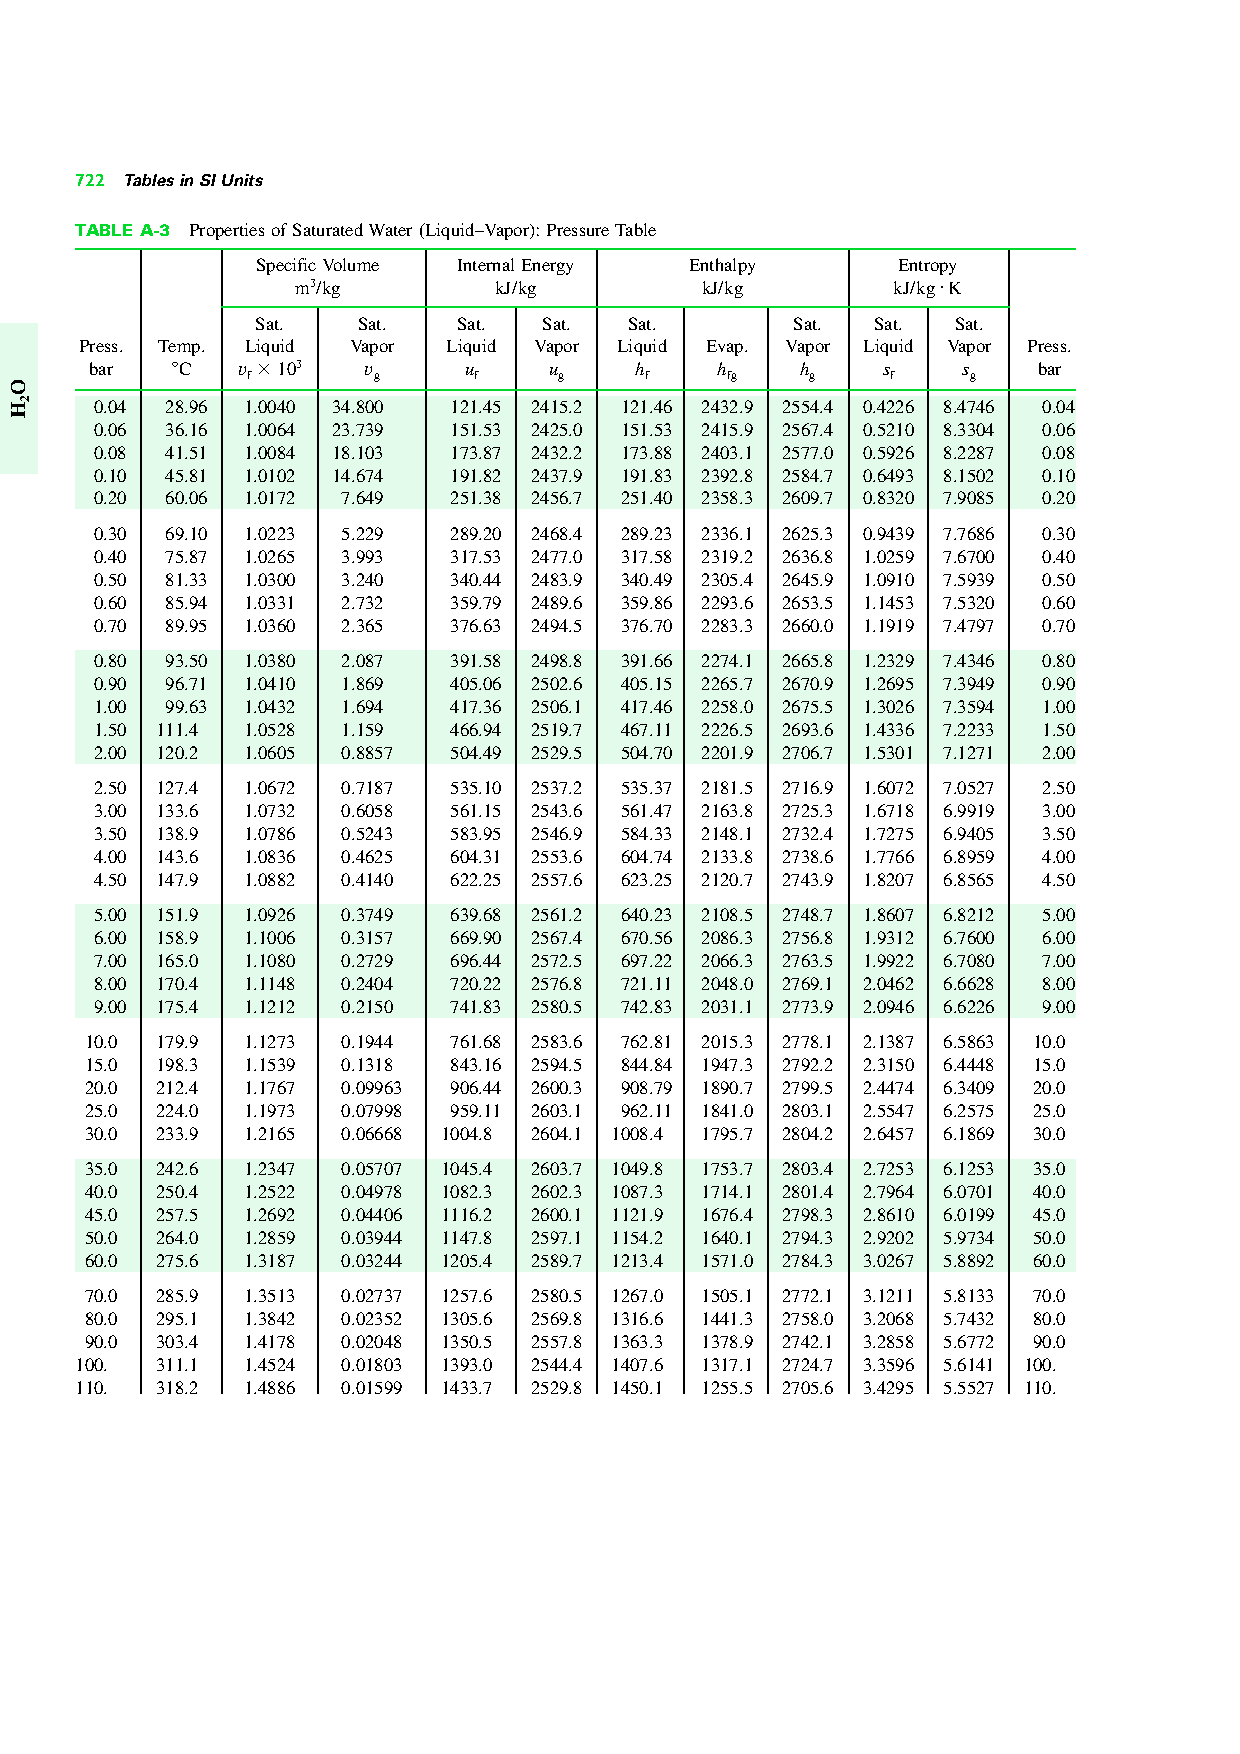
\includegraphics[width=9.5cm,height=9.5cm,clip]{./Pics/WaterSatTable}
   \end{figure}
   \end{center}
\end{frame}


%%%
%%% Slide
%%%
\begin{frame}
  \frametitle{Another option: (b) Superheated Tables}
\scriptsize{From Reference (d):}\vspace{-.8cm}
   \begin{center}
   \begin{figure}
      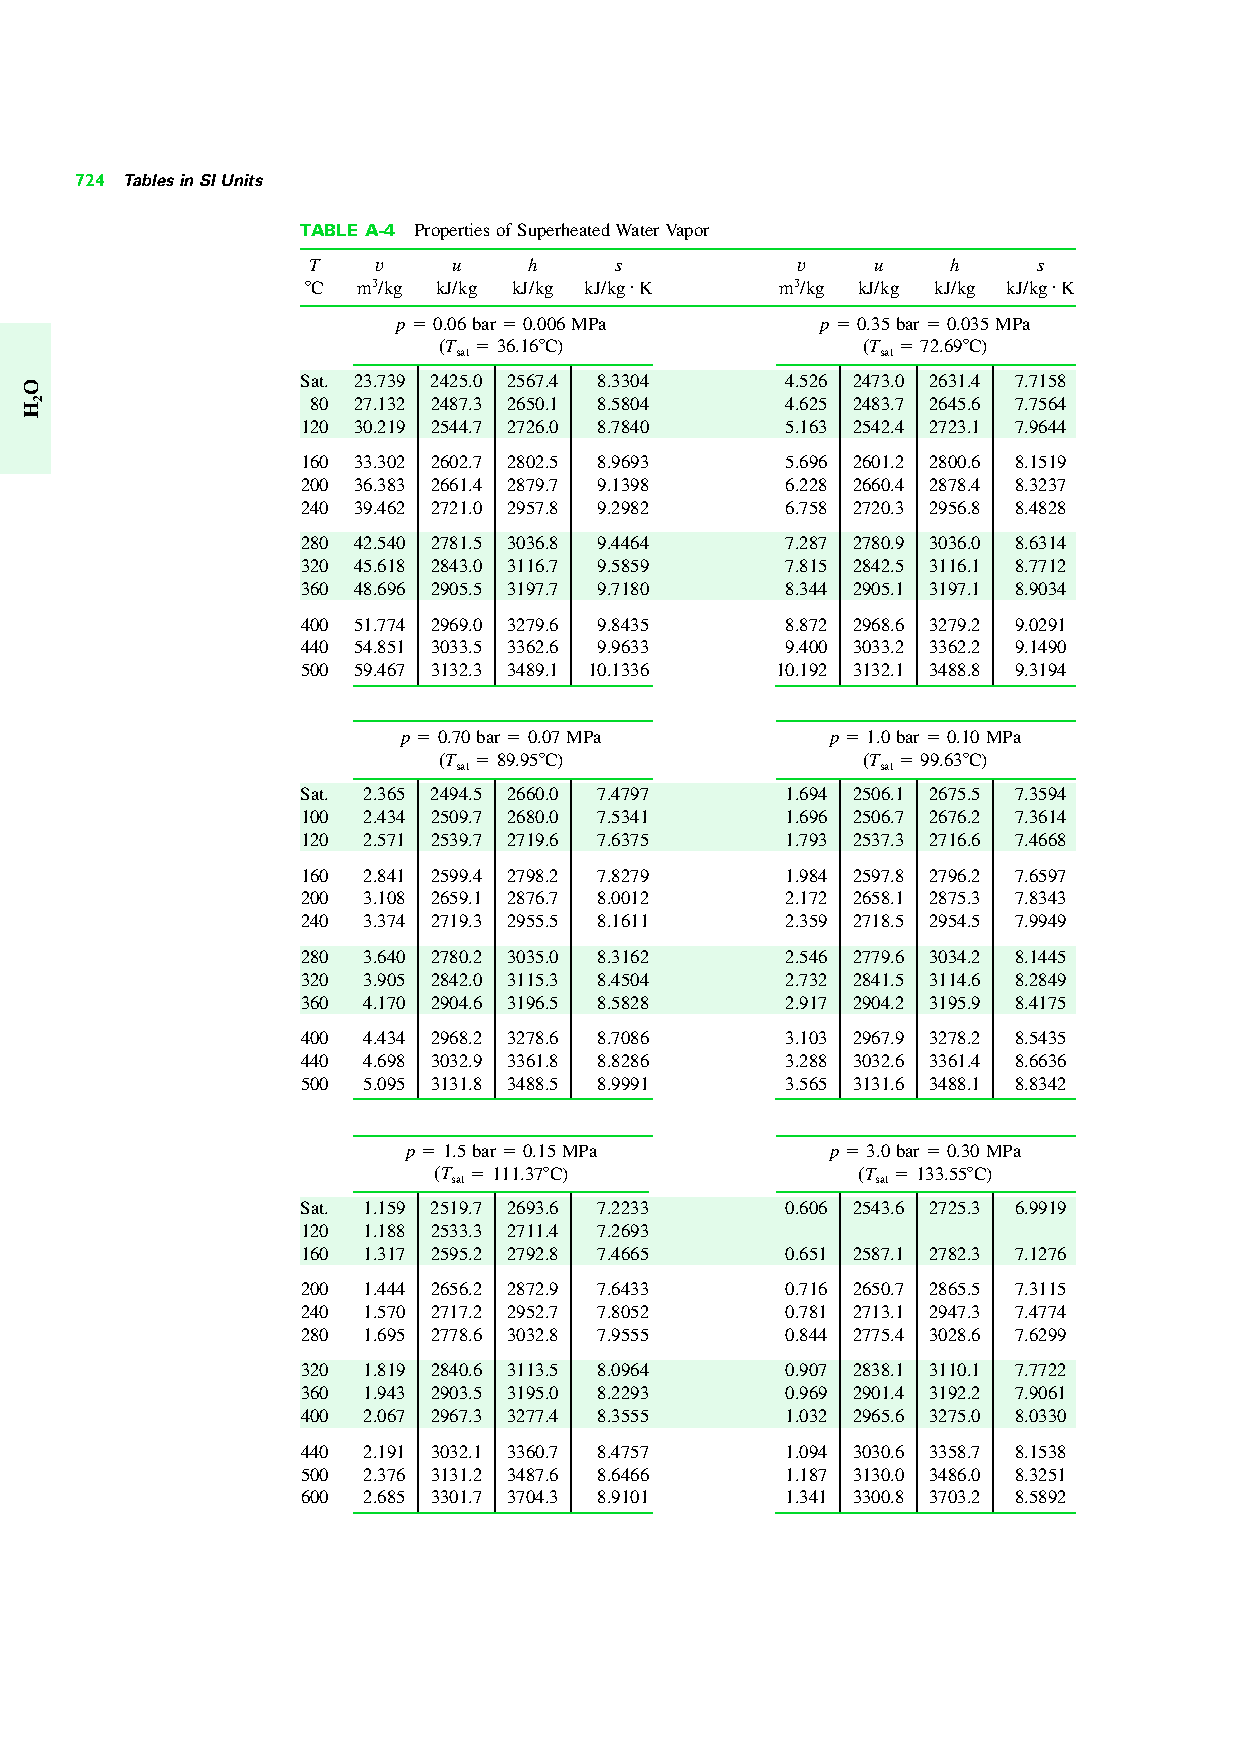
\includegraphics[width=9.5cm,height=9.5cm,clip]{./Pics/Water_SuperheatedTable}
   \end{figure}
   \end{center}
\end{frame}


%%%
%%% Slide
%%%
\begin{frame}
  \frametitle{Another option: Saturated and Superheated Tables}
\noindent
\begin{itemize}
\item <1-> {\bf \textcolor{red}{Example:}} At $P=1.50\;$ bar, the saturated steam has the following thermodynamic properties,
\tiny 
\begin{center}
%\begin{table}[h]
\begin{tabular}{c c|c c c|c c|c c} 
%\hline\hline
$P$ & $T$ & $h_{f}$ &  $h_{fg}$ & $h_{g}$ & $s_{f}$ &  $s_{g}$ & $v_{f}$ & $v_{g}$ \\ 
\hline
1.50 & 111.4 & 467.11 & 2226.5 & 2693.6 & 1.4336 & 7.2233 & 0.0010528 & 1.159 \\
%\hline
\end{tabular}
%\caption{Carnot and Rankine Cycles: From Saturated water and steam tables.}
%\label{Example01_01:Table2}
%\end{table}
\end{center}

\item <3-> But the properties of superheated steam at the same pressure will depend on the temperature $\Rightarrow$ \textcolor{red}{see superheated steam table}. Thus at 1.50 bar $\left(\text{with }T_{\text{sat}}=111.4^{\circ}\text{C}\right)$:
  \visible<3->{\begin{center}\begin{tabular}{ c | c c c}
      $T$    & $v$    & $h$     &    $s$     \\
\hline
      111.4  & 1.159  & 2693.6  &  7.2233    \\
      120.0  & 1.188  & 2711.4  &  7.2693    \\
      160.0  & 1.317  & 2792.8  &  7.4665    \\
      200.0  & 1.444  & 2872.9  &  7.6433    \\
      240.0  & 1.570  & 2952.7  &  7.8052    \\ 
     $\vdots$& $\vdots$&$\vdots$&$\vdots$ \\
  \end{tabular}
  \end{center}
}
\item <2-> {\bf Units:} [$P$] = bar, [$T$] = $^{o}$C, [$h$]= $\frac{kJ}{kg}$, [$s$]=$\frac{kJ}{kg.K}$, [$v$]=$\frac{m^{3}}{kg}$.

\end{itemize}

\end{frame}

%%%% COMMENT
\begin{comment}
%%%
%%% Slide
%%%
\begin{frame}
  \frametitle{Another option: Saturated and Superheated Tables (Linear Interpolation)}
\noindent
\begin{itemize}
\item <2-> Some of the problems in this course involves extracting values from the thermodynamic tables;
\item <3-> And although the tables are very extensive (for most of the materials), sometimes we need values that can not be directly found on them;
\item <4-> In this case, we just operate a {\bf linear interpolation} between neighbour fields;
\item <5-> For example, water-steam at 1.5 bar and 212$^{o}$C. At this pressure, the {\bf saturation temperature} is 111.3$^{o}$C, therefore we know that the fluid (water/steam) is at \textcolor{red}{superheated state} -- \textcolor{red}{$T > T_{\text{sat}}$}
\end{itemize}

\end{frame}

%%%
%%% Slide
%%%

\begin{frame}
  \frametitle{Another option: Saturated and Superheated Tables (Linear Interpolation)}
\noindent
\begin{itemize}
\item <1-> Thus at 1.5 bar and 212$^{\circ}$C, enthalpy and entropy of superheated steam are within the following interval:
  \visible<1->{\begin{center}\begin{tabular}{ c | c c c}
      $T$    & $v$    & $h$     &    $s$     \\
      \textcolor{red}{200.0}  & 1.444  & \textcolor{red}{2872.9}  &  7.6433    \\
      \textcolor{red}{240.0}  & 1.570  & \textcolor{red}{2952.7}  &  7.8052    \\ 
  \end{tabular}
  \end{center}
}
\item<2-> The enthalpy at 212$^{o}$C can be calculated as,
\visible<3->{\begin{tabular}{ l l }
\scriptsize $\Delta T=T_{2}-T_{1}=240-200^{o}$C   & \scriptsize $\longleftrightarrow$  $\Delta h=h_{2}-h_{1}=2952.7-2872.9=79.8\frac{kJ}{kg}$ \\
\scriptsize $\Delta T^{\star} = T_{2} - T^{\star}= 240 - 212^{\circ}$C & \scriptsize $\longleftrightarrow$  $\Delta h^{\star}= h_{2} - h^{\star}= 2952.7 - h^{\star}$\\    
\end{tabular}}
\item <4-> $\Delta h^{\star}=55.86\frac{kJ}{kg}$ 
\item <4-> Thus $\Delta h^{\star}= h_{2}-h^{\star} \longrightarrow h\left(T=212^{\circ}C\right)=h^{\star}=2896.84\frac{kJ}{kg}$.
\item<5-> Similarly for entropy: $s\left(T=212^{\circ}C\right)=s^{\star}=7.6919\frac{kJ}{kg.K}$.
\end{itemize}

\end{frame}

\end{comment}

%%%
%%% Slide
%%%

\begin{frame}
  \frametitle{Third Option: PVT Software and Website}
\noindent
\begin{itemize}
   \item<1-> \href{http://www.weatherford.com/doc/wft183650}{PVTflex$^{TM}$};
   \item<1-> \href{http://www.kbcat.com/infochem-software/flow-assurance-software-multiflash/pvt-simulation}{Multiflash$^{TM}$};
   \item<1-> \href{https://www.honeywellprocess.com/en-US/explore/products/advanced-applications/unisim/Pages/default.aspx}{UniSim – Software for Process Design and Simulation};
   \item<1-> \href{http://webbook.nist.gov/chemistry/fluid/}{NIST Website}
   \item<1-> etc.
\end{itemize}

\end{frame}



%%%           %%%
%%%  SECTION  %%% 
%%%           %%%
\section{Vapour Power Systems}

%%% SUBSECTION
\subsection{Introduction}

%%%% COMMENT
\begin{comment}
%%%
%%% Slide
%%%
\begin{frame}
 \frametitle{Introduction to Vapour and Gas Power}
    \begin{figure}%
     \begin{center}
      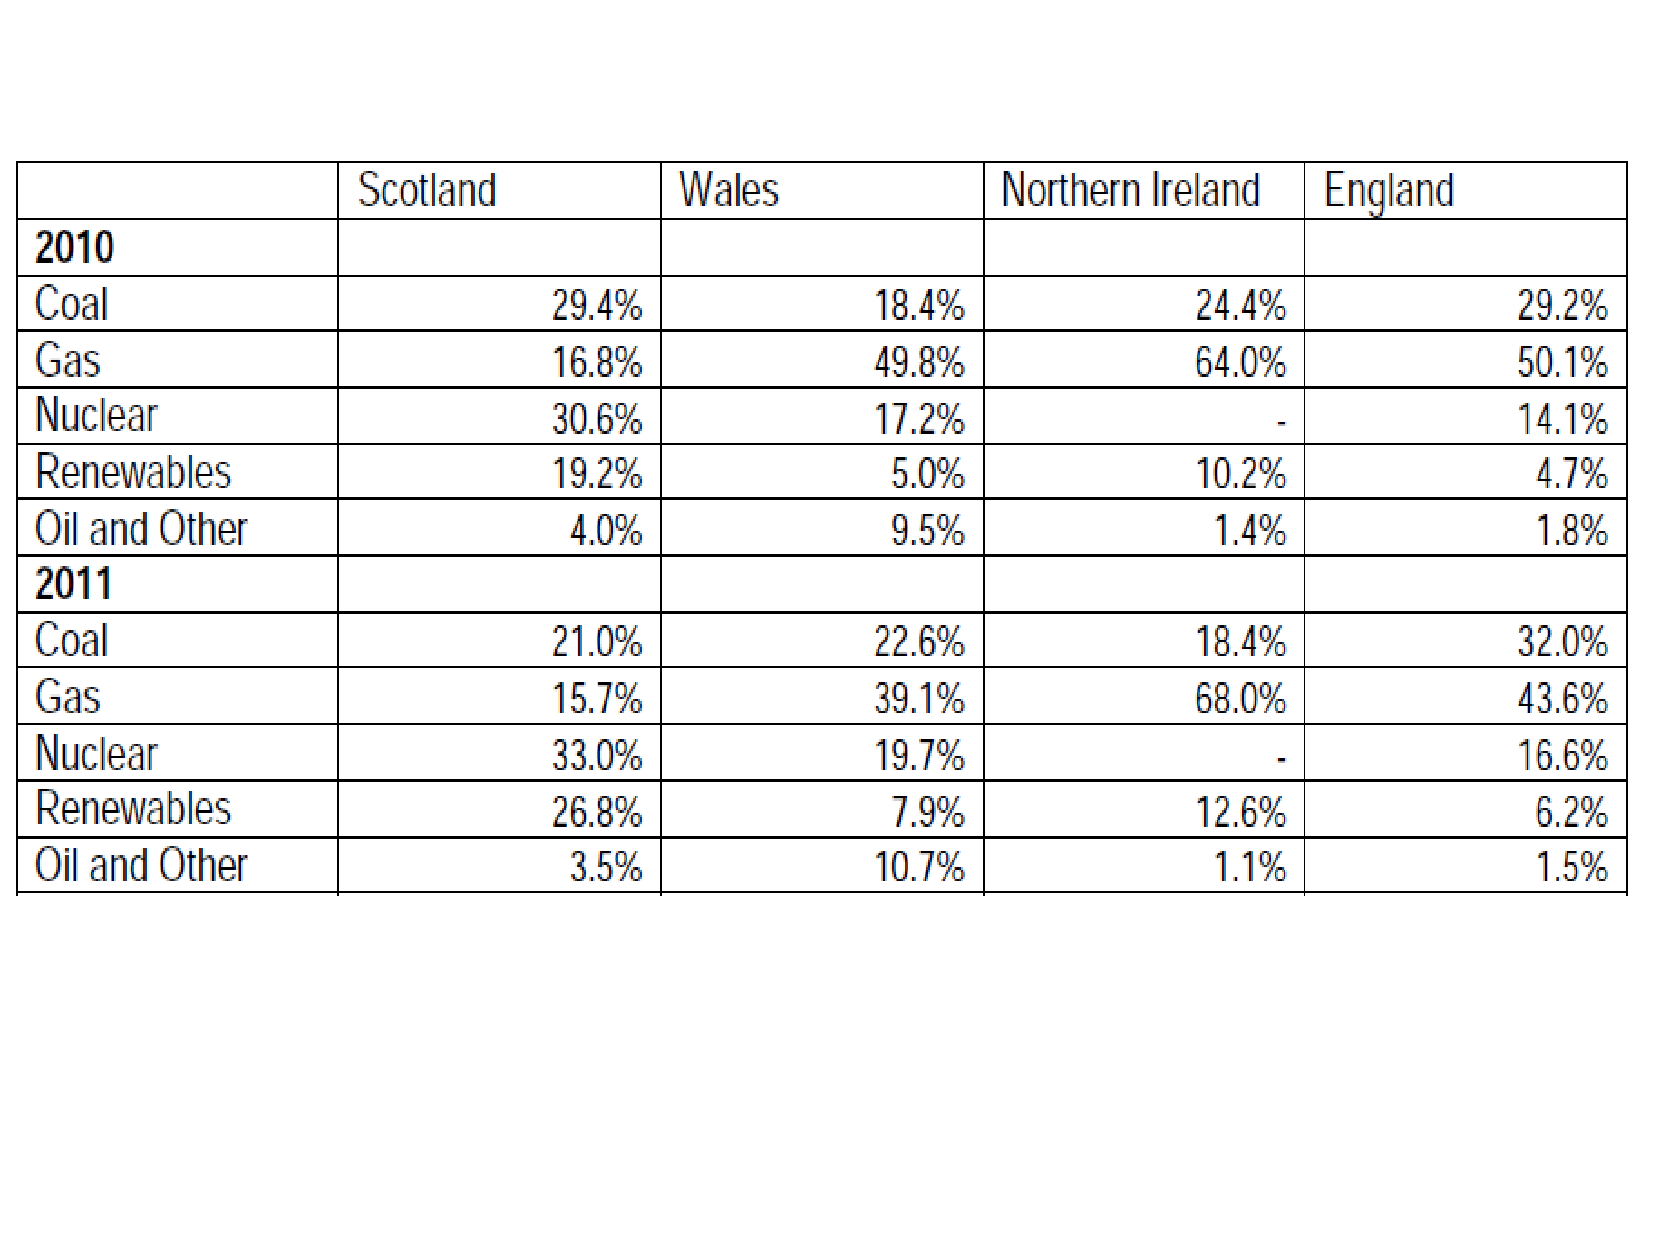
\includegraphics[width=9.cm,clip]{./Pics/Energy_Share_UK}
     \end{center}
    \end{figure}
\vspace{-2cm}
%\scriptsize
\textcolor{blue}{Fuel used in electricity generation and electricity supplied. (\href{https://www.gov.uk/government/organisations/department-of-energy-climate-change/series/electricity-statistics}{https://www.gov.uk/government/organisations/department-of-energy-climate-change/series/electricity-statistics})}
 \normalsize
\end{frame}

\end{comment}


%%%
%%% Slide
%%%
\begin{frame}
 \frametitle{Introduction to Vapour and Gas Power}

    \begin{center}
     \begin{table}
       \begin{tabular}{l c c c}
    \hline
    \textcolor{blue}{Power Plant} & \textcolor{blue}{Renewable}  & \textcolor{blue}{Thermodynamic} \\
    \textcolor{blue}{Type}        & \textcolor{blue}{Source}     & \textcolor{blue}{Cycle}         \\
    \hline
      Coal                        &   No                         & Rankine  \\
      Natural Gas                 &   No                         & Brayton  \\
      Nuclear                     &   No                         & Rankine  \\
      Oil                         &   No                         & Rankine  \\
      Biomass                     &   Yes                        & Rankine  \\
      \textcolor{red}{Geothermal} &   Yes                        & \textcolor{red}{Rankine}  \\
      Solar                       &   Yes                        & Rankine  \\
      Hydroelectric               &   Yes                        & None     \\
      Wind                        &   Yes                        & None     \\
      Currents, tides and         &   Yes                        & None     \\
      waves                       &                              &          \\
    %\hline
    %\hline
      \end{tabular}
     \end{table}
    \end{center}
\end{frame}

%%%
%%% Slide
%%%
\begin{frame}
 \frametitle{Introduction to Vapour and Gas Power}
 %\scriptsize

    \begin{enumerate}%\scriptsize
     \item <1-> While coal, natural gas, and nuclear still play important roles as energy sources, contributions from wind power, solar power, and other renewable sources are expected to be increasingly significant up to 2050;
     \item <2-> This table shows that thermodynamic cycles are crucial for a number of power plant types that employ renewable and non-renewable sources;
     \item <3-> The basic building block of vapour power systems is the \textcolor{blue}{Rankine cycle};
     \item <4-> Energy sources based on thermal-cycles (YouTube videos):
        \begin{itemize}%\scriptsize
           \item \href{http://www.youtube.com/watch?v=_UwexvaCMWA}{\textcolor{blue}{Nuclear Power Plants (NPP)}};
           \item \href{http://www.youtube.com/watch?v=0mjT8ETB128}{\textcolor{blue}{Coal-Fired Stations}};
           \item \href{http://www.youtube.com/watch?v=oi1TRbiE_Kw}{\textcolor{blue}{Gas Turbine Combined Cycle Power Plant}};
           \item \href{https://www.youtube.com/watch?v=kjpp2MQffnw}{\textcolor{blue}{Geothermal Power Plant}}.
        \end{itemize}
    \end{enumerate}
 \normalsize
\end{frame}


%%%
%%% Slide
%%%
\begin{frame}
 \frametitle{A Few Definitions}
 %%\scriptsize
 \begin{itemize}
  \item <1-> A \textcolor{blue}{cycle} is defined as a repeated series of operations occurring in a certain order. A system is said to have undergone a cycle if it returns to its initial state at the end of the process.  Cycles can be classified as ideal (where there is no heat losses) and real. 
  \item <2-> In \textcolor{blue}{gas cycles}, the working fluid remains in the gas phase throughout the cycle (e.g., air).
  \item <3-> In \textcolor{blue}{vapour cycles}, the working fluid exists as a vapour for part of the cycle and a liquid for the other part -- i.e., \red{the working fluid is alternately vaporised and condensed}.
  \item <4-> Steam is the most common working fluid in vapour power cycles as it has many desirable characteristics: low cost, availability and high enthalpy of vaporisation.
 % \item <5-> Coal, nuclear and natural gas power plants are examples of steam power plants. Each utilises a different type of fuel to supply heat to the steam cycle. 
  \item <5-> In \textcolor{blue}{closed cycles}, after each pass through the cycle the working fluid remains within the system.
  \item <6-> In \textcolor{blue}{open cycles}, after a few (or a single) pass through the cycle the working fluid is replaced by a fresh working fluid.
 \end{itemize}
 %\normalsize
\end{frame}


%%%% COMMENT
\begin{comment}
%%%
%%% SUB-SECTION
%%%
\subsection{Carnot Engines / Cycles}


%%%
%%% Slide
%%%
\begin{frame}
 %\scriptsize
 \frametitle{The Carnot Cycle}
  \begin{columns}
   \begin{column}[c]{0.6\linewidth}
    \begin{enumerate}[(a)] \scriptsize
     \item <1-> A \blue{heat engine} is a closed system that converts heat to work and operates in a cycle;
     \item <2-> A \blue{Carnot cycle} has four reversible steps, alternating \blue{isothermal} (and \blue{isobaric:} 4-1, 2-3) and frictionless \blue{adiabatic} (i.e., \blue{isentropic:} 1-2, 3-4):
       \begin{enumerate}[(i)]\scriptsize
         \item <3-> {\it Step 1-2}: \blue{Steam} is \red{isentropically} expanded to $T_{2}$ and $P_{2}$;
         \item <4-> {\it Step 2-3}: Heat is rejected at \red{constant pressure} $\left(P_{2}\right)$ \red{and temperature} $\left(T_{2}\right)$. During this step, steam becomes wetter and cooled;
         \item <5-> {\it Step 3-4}: Wet steam is \red{isentropically} compressed until the steam returns to its original state at $T_{1}$ and $P_{1}$ (saturated liquid);
         \item <6-> {\it Step 4-1}: \blue{Boiling water} at temperature $T_{1}$ is heated to form wet steam $\left(\right.$dryness fraction $x_{1}\left.\right)$. Heat is then absorbed at \red{constant temperature} $\left(T_{1}\right)$ \red{and pressure} $\left(P_{1}\right)$;
       \end{enumerate}
     \item <7-> The efficiency of the \blue{Carnot cycle} is given by:
          \visible<7->{\begin{equation}
             \blue{\eta_{\text{Carnot}}} = \frc{\text{Work Done}}{\text{Heat Supplied}} \blue{= 1 - \frc{T_{2}}{T_{1}}}
          \end{equation}}
    \end{enumerate} 
   \end{column}
   \begin{column}[c]{0.4\linewidth}
   \begin{figure}%
    \begin{center}
     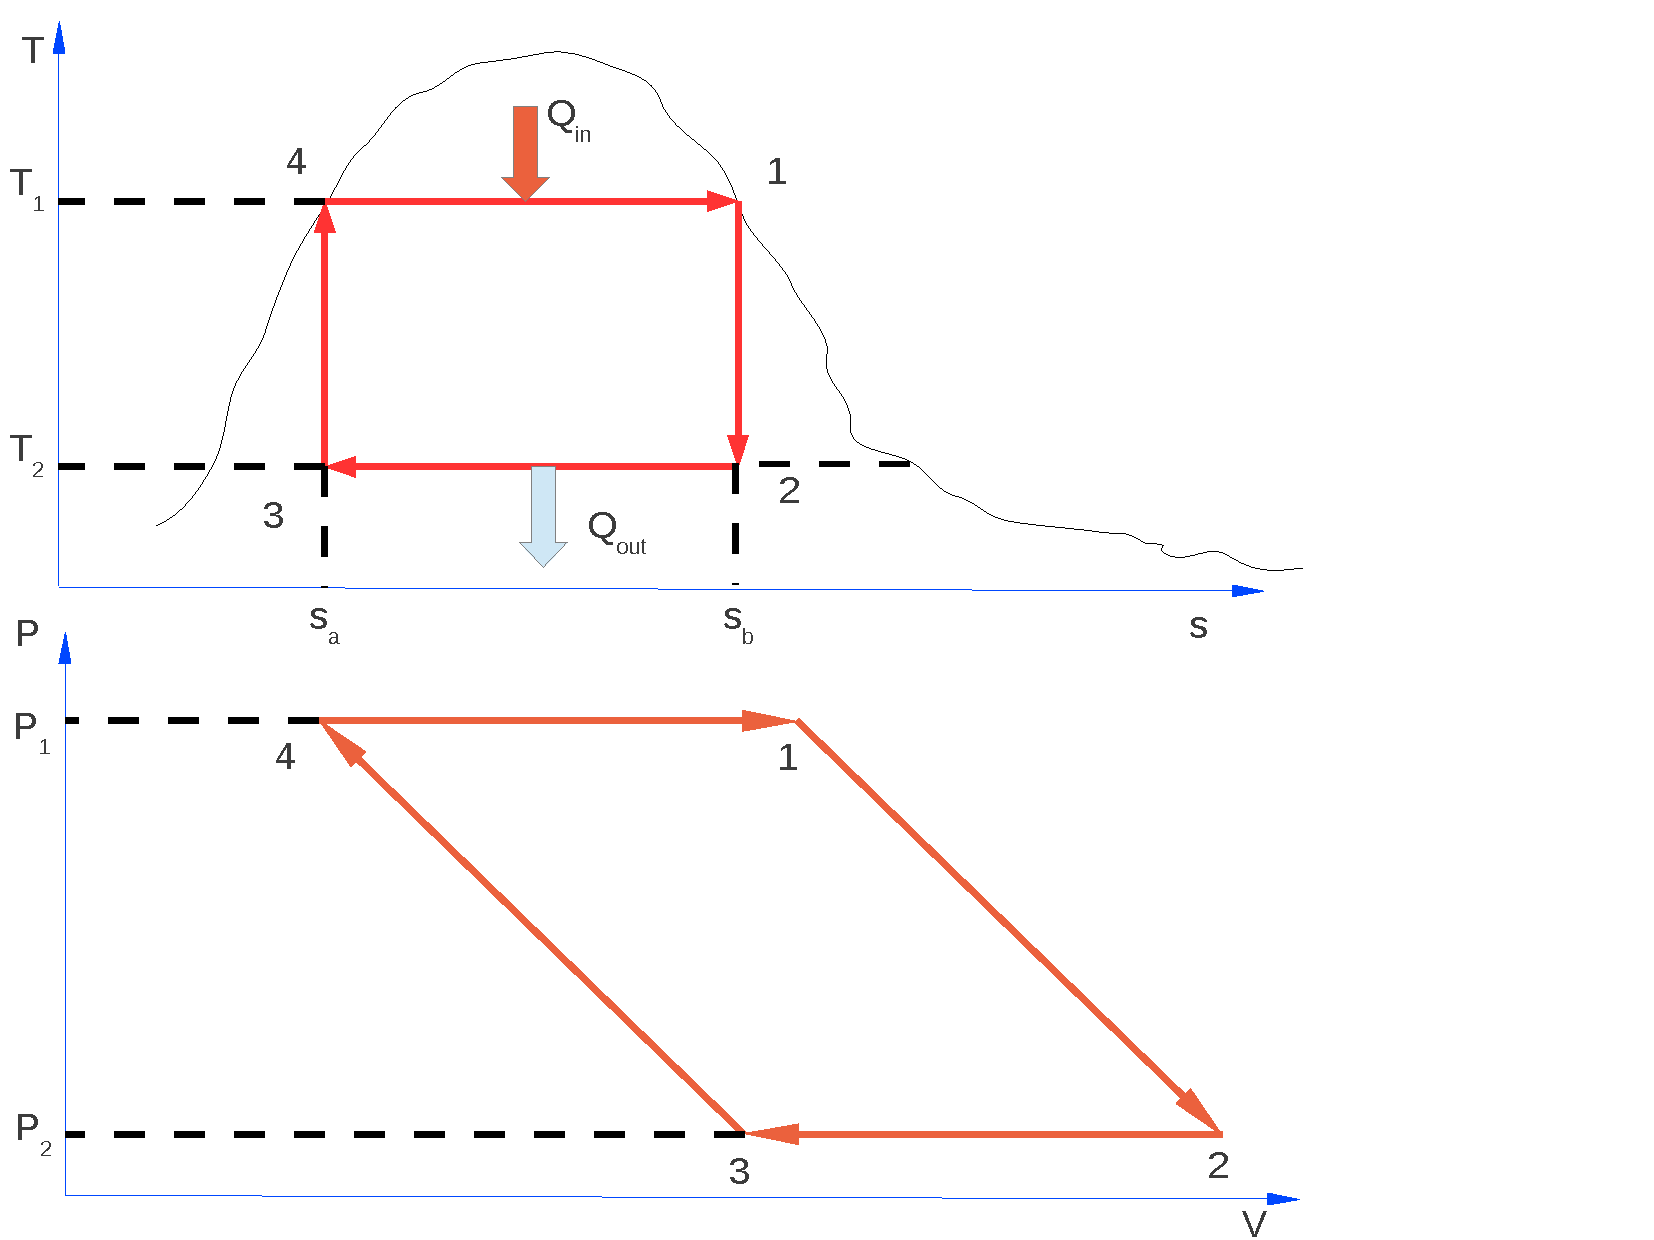
\includegraphics[width=5.5cm,clip]{./Pics/Carnot_PV_TS}
    \end{center}
   \end{figure}    
   \end{column}
  \end{columns}
 \normalsize
\end{frame}

%%%
%%% Slide
%%%
\begin{frame}
 \frametitle{Limitations of the Carnot Cycle}
 %\scriptsize
 \begin{enumerate}[(a)]
  \item <1-> The \blue{Carnot cycle} is thermodynamically simple and has the \red{highest thermal efficiency} for a given temperature gradient;
  \item <2-> It is however {\it difficult to operate in practice} due to:
  \begin{enumerate}[(i)] %\scriptsize
   \item <3-> It is difficult to \underline{compress a wet vapour isentropically} to the saturated state (as required by the process 3-4);
   \item <4-> It is difficult to \underline{control the quality of the condensate} produced by the condenser to reach state 3;
   %\item <5-> The \blue{efficiency is greatly affected by $T_{1}$} at which heat is transferred to the working fluid. As the critical temperature of steam is 374$^{\circ}$C therefore, if the cycle is to be operated in the wet region, the maximum possible temperature is severely limited;
   \item <6-> The cycle is even more difficult to operate in practice with superheated steam due to the necessity to \blue{supply superheated steam at constant temperature instead of constant pressure} (as it is usual in industrial plants);
   \item <7-> \red{\it In a practical cycle, limits of pressure and volume are easier to be obtained than limits of temperature}; 
   \item <8-> Therefore \blue{\underline{no practical engine operates in the Carnot cycle}}, although all modern cycles aspire to achieve it.
          \begin{displaymath}
             \visible<9->{\blue{\eta_{\text{Carnot}}} = \frc{\text{Work Done}}{\text{Heat Supplied}}\blue{= 1 - \frc{T_{2}}{T_{1}}}} \visible<10->{ = \bf{\red{\eta_{\text{max}}}}}
          \end{displaymath}
  \end{enumerate}
 \end{enumerate}
 \normalsize
\end{frame}

\end{comment}

%%%
%%% SUB-SECTION
%%%
\subsection{Rankine Engines / Cycles}

%%%
%%% Slide
%%%
\begin{frame}
 \frametitle{Rankine Cycle}
 %\scriptsize
 \begin{columns}
   \begin{column}[c]{0.5\linewidth}
    \begin{figure}%
     \begin{center}
      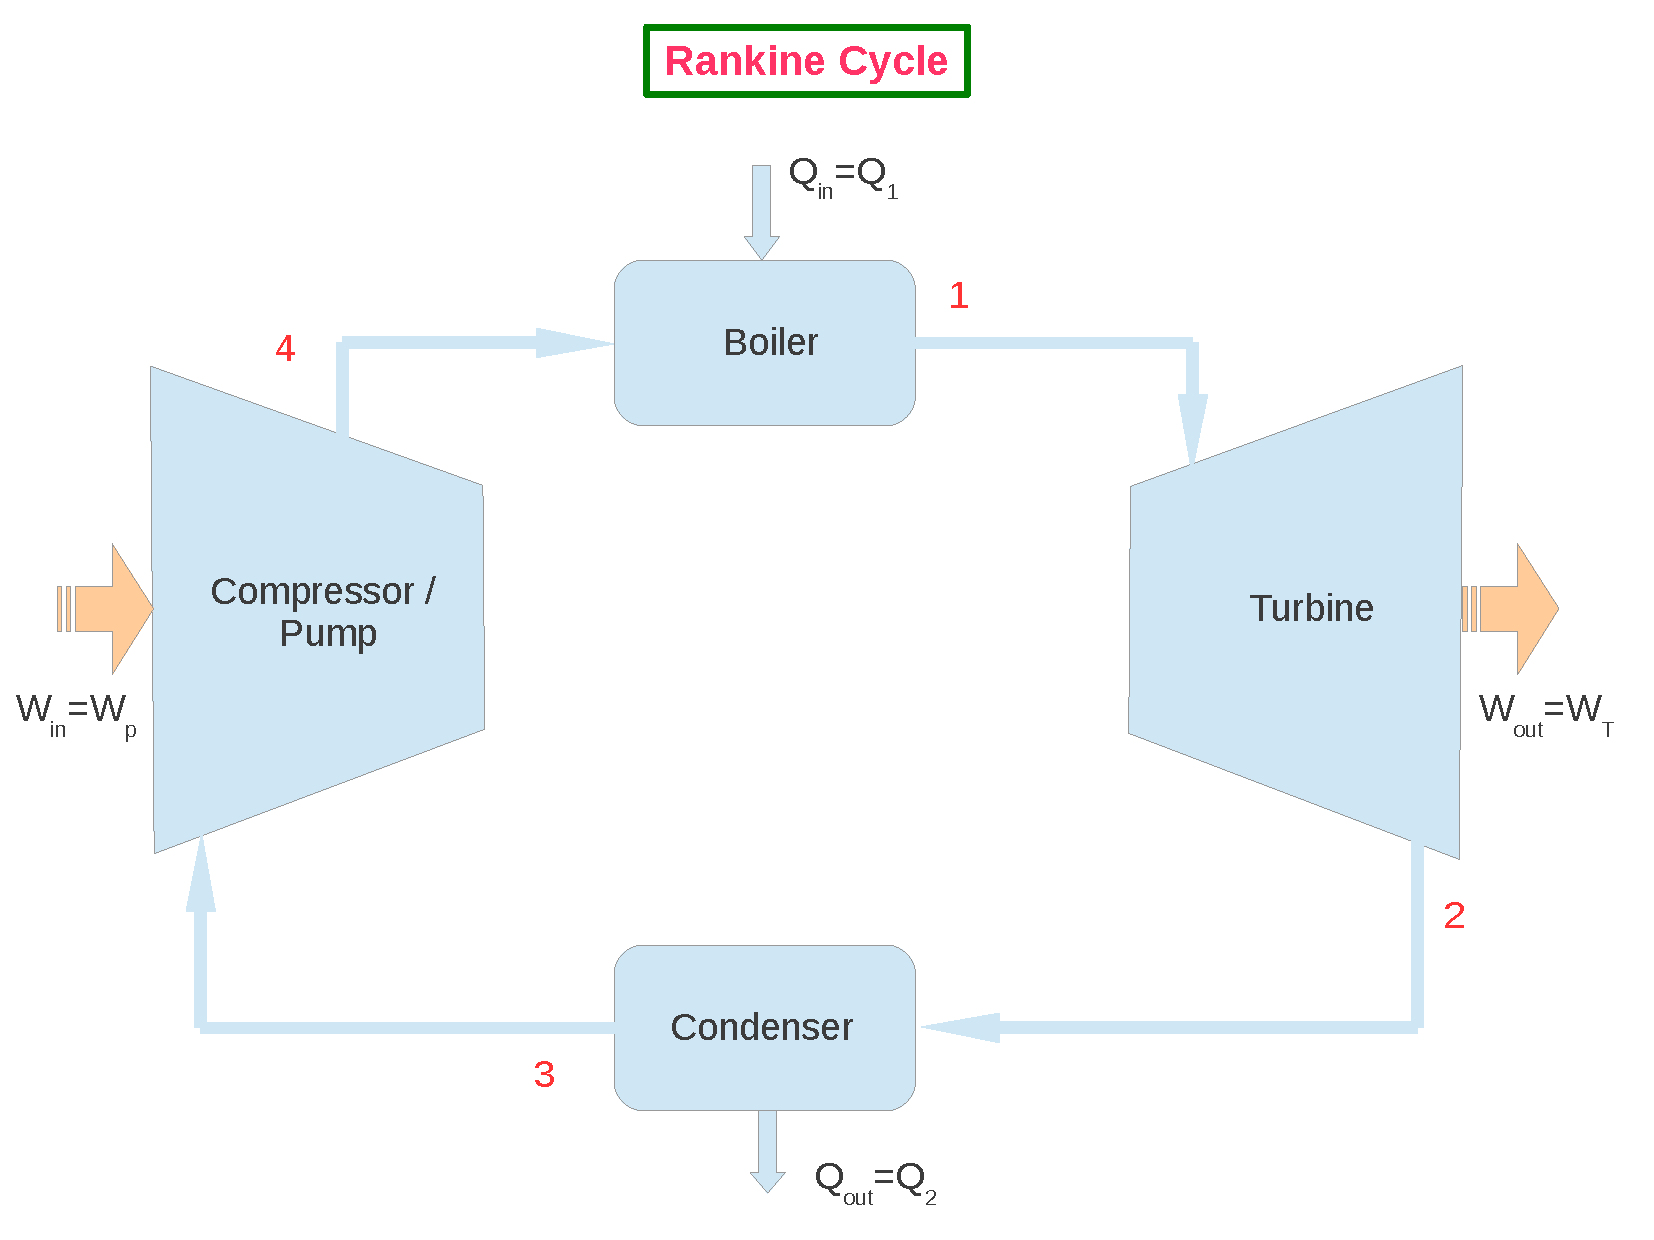
\includegraphics[width=6.5cm,clip]{./Pics/Simple_Rankine_Cycle}
     \end{center}
    \end{figure}  
   \end{column}
   \begin{column}[l]{0.5\linewidth}
    \begin{enumerate}[(a)]\scriptsize
     \item<1->\textcolor{blue}{Rankine Cycle} (RC) is the ideal cycle for vapour power plants;
     \item<2-> It does not involve any internal irreversibilities and consists of the following four processes:
     \begin{enumerate}[(i)]\scriptsize
      \item<3-> \textcolor{red}{Process 1-2}: reversible adiabatic (i.e., \blue{isentropic}) expansion in the turbine (or steam engine);
      \item<4-> \textcolor{red}{Process 2-3}: constant-pressure heat transfer in the condenser;
      \item<5-> \textcolor{red}{Process 3-4}: reversible adiabatic (i.e., \blue{isentropic}) pumping process in the feed pump;
      \item<6-> \textcolor{red}{Process 4-1}: constant-pressure heat transfer in the boiler.  
     \end{enumerate}
     \item<7-> Efficiency of the \blue{RC} can be expressed as:
       \visible<7->{\begin{eqnarray}
          \blue{\eta_{\text{Rankine}}} &=& \frc{W_{\text{net}}}{Q_{1}} = \frc{W_{T}-W_{P}}{Q_{1}}\nonumber \\
                                    &=& \frc{\left(h_{1}-h_{2}\right)-\left(h_{f4}-h_{f3}\right)}{h_{1}-h_{f4}} \nonumber \\
                                    &=& \blue{\frc{h_{1}-h_{2}}{h_{1}-h_{f4}}} 
       \end{eqnarray}}
    \end{enumerate}
   \end{column}
  \end{columns}
 \normalsize
\end{frame}


%%%
%%% Slide
%%%
\begin{frame}
 \frametitle{Rankine Cycle: {\it Pv}, {\it Ts} and {\it hs} Diagrams}
 %\scriptsize
 \begin{columns}
%
   \begin{column}[l]{0.45\linewidth}
    \begin{figure}%
     \begin{center}
      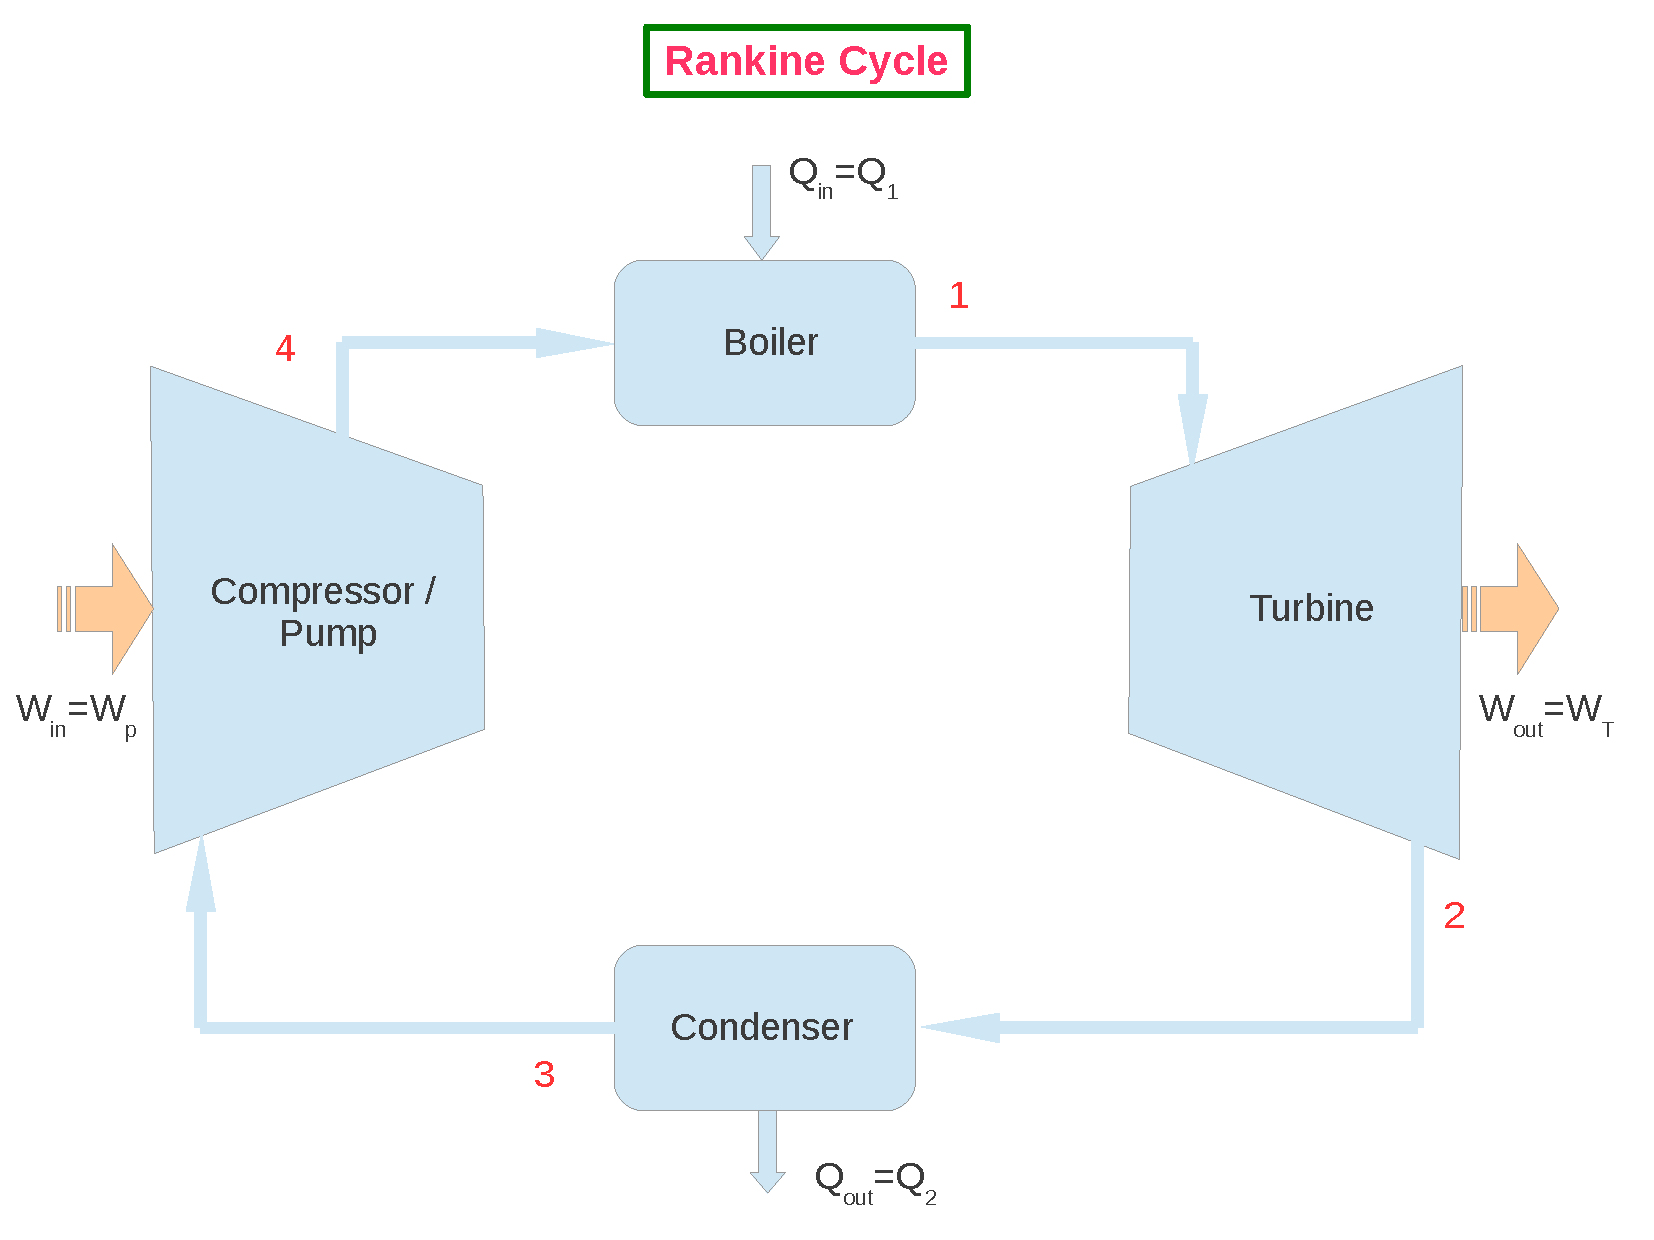
\includegraphics[width=5.5cm,clip]{./Pics/Simple_Rankine_Cycle}
     \end{center}
    \end{figure} 
    \begin{block}{\begin{center}Quality of the Vapour\end{center}}
       \begin{equation}\scriptsize
         \blue{x_{j} = \frc{\Psi_{j}-\Psi_{f}}{\Psi_{g}-\Psi_{f}}} \;\;\;\text{with }\Psi=\left\{h,s\right\}
       \end{equation}
    \end{block}
   \end{column}
%
   \begin{column}[c]{0.55\linewidth}
    \begin{figure}%
     \begin{center}
      \visible<2->{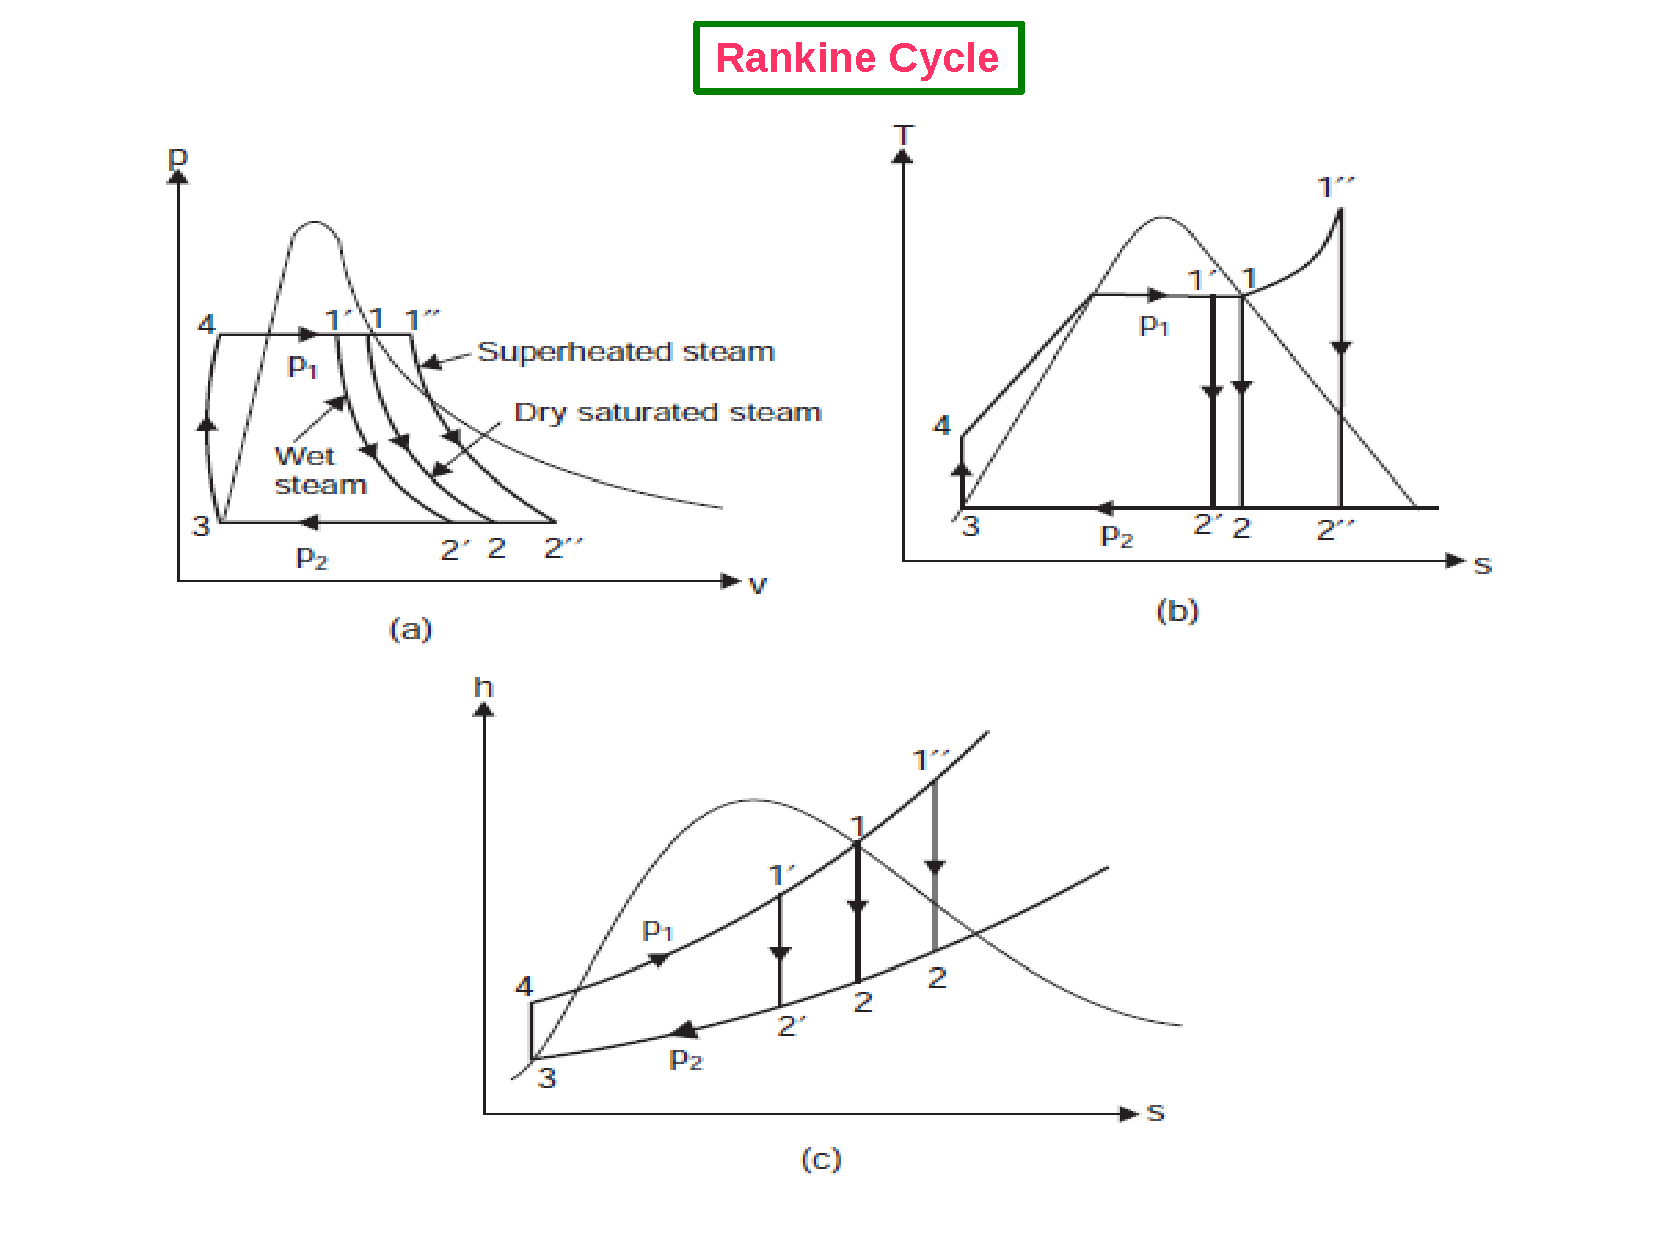
\includegraphics[width=7.5cm,clip]{./Pics/Simple_Rankine_Cycle_Diagrams}}
     \end{center}
    \end{figure}  
   \end{column}
  \end{columns}
\end{frame}


%%%
%%% Slide
%%%
\begin{frame}
 \frametitle{Ideal {\it versus} Actual Rankine Cycles}
   \begin{columns}
      \begin{column}[c]{0.5\linewidth}
         \begin{enumerate}\scriptsize
             \item<1-> Differences between actual and ideal RC are mainly due to \blue{fluid friction} resulting in \blue{pressure drop in the boiler, condenser and pipes};
             \item<2-> Steam leaves the boiler at a pressure lower than expected; 
             \item<3-> \underline{Fluid pressure at the turbine inlet} is also \underline{lower than that at the boiler exit} due to pressure drop between pipes; 
             \item<4-> Pressure drop in the \blue{condenser} is usually \underline{negligible}; 
             \item<5-> In order to mitigate these pressure drops throughout power cycles, water must be pumped to a pressure higher than the required in the ideal cycle. Thus, a more powerful pump (and therefore larger work input to the pump) is needed, increasing the energy cost.  
         \end{enumerate}\scriptsize
         \visible<6->{\begin{block}{\begin{center}Efficiencies of Turbines and Pumps\end{center}}
           \begin{eqnarray}\scriptsize
              && \blue{\eta_{T}=} \frc{W_{T,a}}{W_{T,s}} = \blue{\frc{h_{2}-h_{1}}{h_{2s}-h_{1}}} \\
              && \blue{\eta_{P}=} \frc{W_{P,s}}{W_{P,a}} = \blue{\frc{h_{4s}-h_{3}}{h_{4}-h_{3}}}
           \end{eqnarray}
         \end{block}}
      \end{column}
      \begin{column}[c]{0.5\linewidth}
         \vbox{
           \hbox{\hspace{.5cm}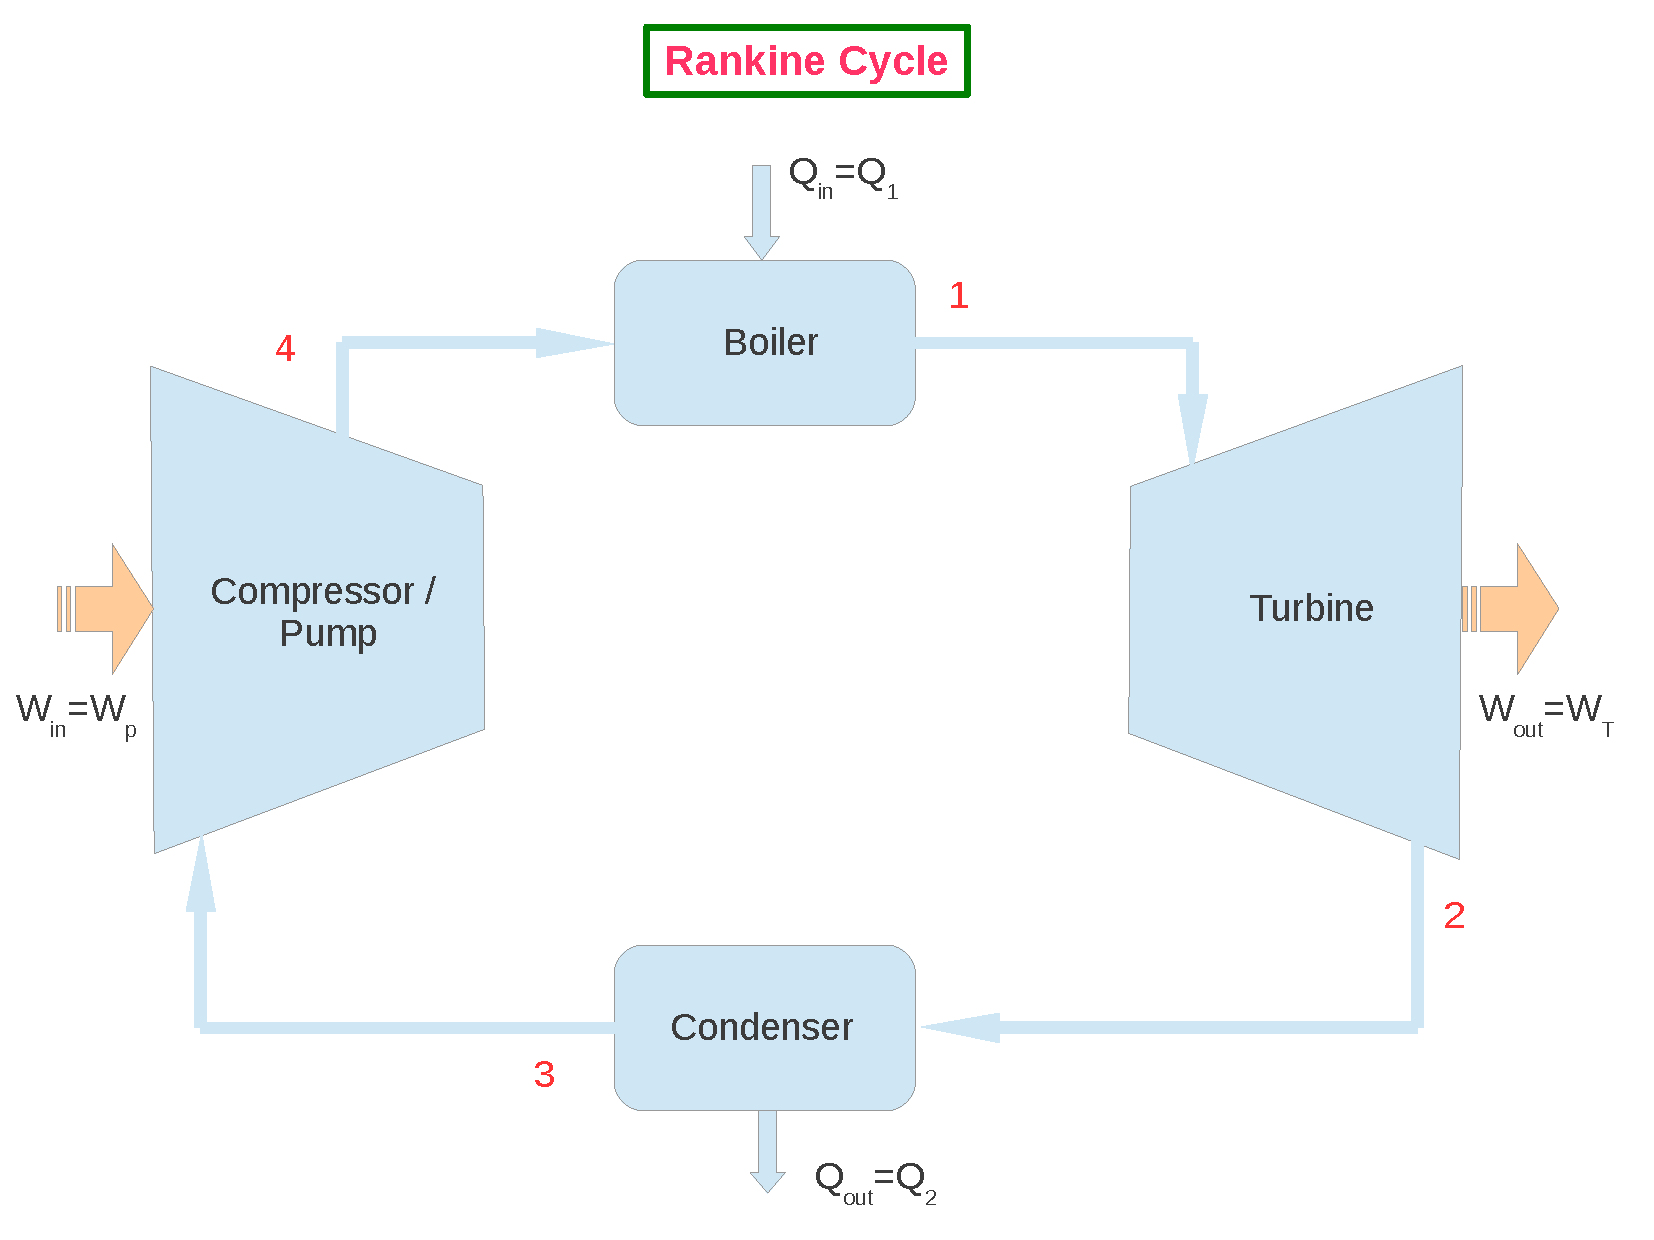
\includegraphics[width=5.cm,clip]{./Pics/Simple_Rankine_Cycle}}
           \vspace{-0.1cm}
           \hbox{\hspace{.5cm}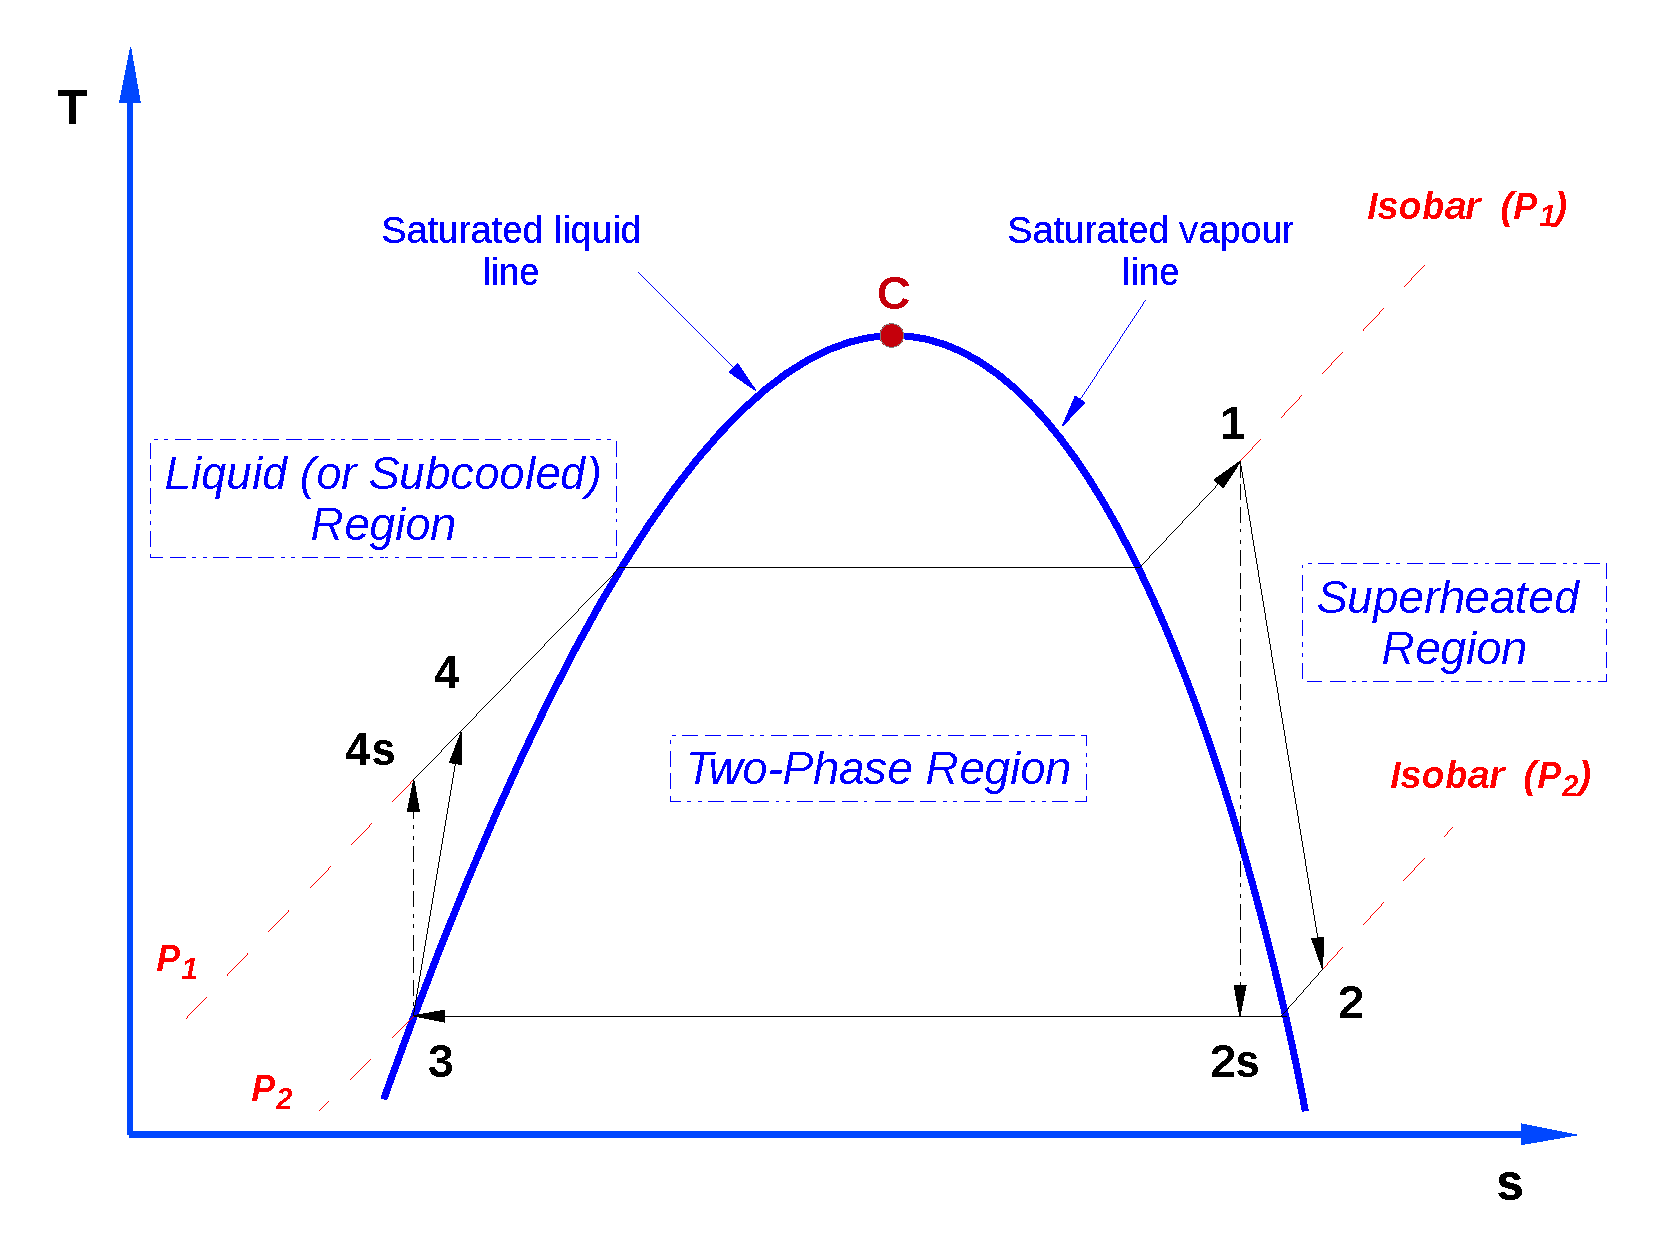
\includegraphics[width=5.5cm,clip]{./Pics/Ideal_Real_Rankine}}
         }
      \end{column}
   \end{columns}
 \normalsize
\end{frame}

%%%
%%% Slide
%%%
\begin{frame}
 \frametitle{Improving the Efficiency of the Rankine Cycles}
   \begin{columns}
      \begin{column}[c]{0.5\linewidth}
         \begin{enumerate}\scriptsize
            \item<1-> The efficiency of the Rankine cycle may be improved by:
              \begin{enumerate}[(a)]\scriptsize
                 \item <1-> Increasing the average temperature at which heat is transferred to the working fluid in the boiler or;
                 \item <1-> Reducing the temperature at which the heat is transferred from the working fluid in the condenser;
              \end{enumerate} 
            \item <2-> This can be achieved with:
              \begin{enumerate}[(a)]\scriptsize
                 \item <2-> Increasing boiler pressure;
                 \item <2-> Use of superheated steam;
                 \item <2-> Reducing condenser pressure.
              \end{enumerate}
            \item <3-> The thermal efficiency can be improved by
              \begin{enumerate}[(a)]\scriptsize
                 \item <3-> Regenerative feed heating;
                 \item <3-> \blue{Reheating of steam};
                 \item <3-> Water extraction;
                 \item <3-> Using binary-vapour
              \end{enumerate}
         \end{enumerate}  
      \end{column}
      \begin{column}[c]{0.5\linewidth}
         \visible<2->{\begin{figure}%
           \begin{center}
              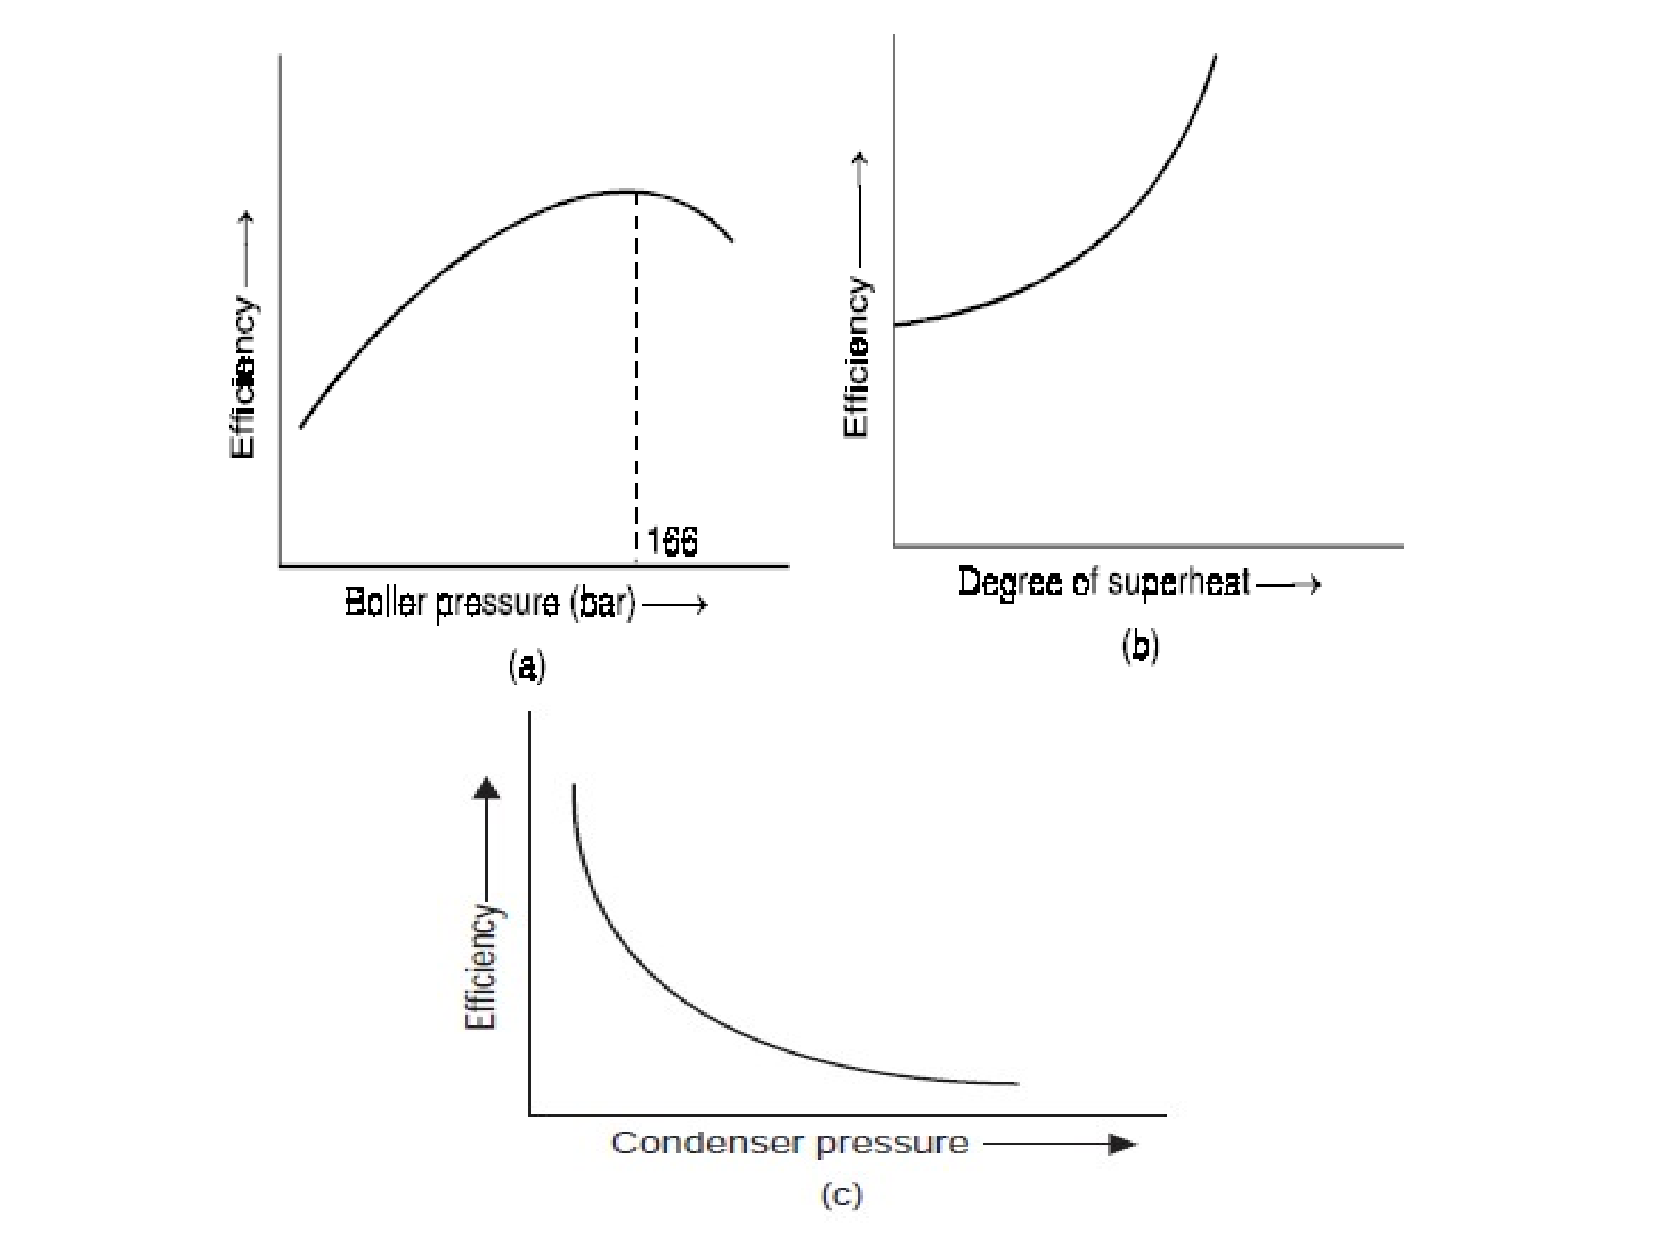
\includegraphics[width=7.cm,clip]{./Pics/Rankine_Improving_Efficiency}
           \end{center}
         \end{figure}}
      \end{column}
   \end{columns}
 \normalsize
\end{frame}

%%%
%%% EXAMPLES
%%%

%%%
%%% Slide
%%%
\begin{frame}
 \frametitle{Example 1: Rankine efficiency}
 %\scriptsize
    Steam (dry and saturated) is supplied by the boiler at 15 bar and the condenser pressure is 0.4 bar. Calculate the Rankine efficiency of the cycle. Neglect the pump work.
\end{frame}

%%%
%%% Slide
%%%
\begin{frame}
 \frametitle{Example 2: Ideal Rankine Cycle}
 %\scriptsize
Water is the working fluid in an ideal Rankine cycle. Dry saturated vapour enters the turbine at 16 MPa, and the condenser pressure is 8 kPa. The mass flow rate of steam entering in the turbine is 120 kg/s. Calculate:
\begin{enumerate}[(a)]
\item the net power developed (in MW);
\item rate of heat transfer to the steam passing through the boiler (in MW);
\item thermal efficiency;
\item mass flow rate of the condenser cooling water (in kg/s), if the cooling water undergoes a temperature increase of 18$^{\circ}$C with negligible pressure change in passing through the condenser. Assume that the heat capacity at constant pressure $\left(\text{C}_{\text{p}}\right)$ of the cooling water is 4.18 $\frac{\text{kJ}}{\text{kg.}^{\circ}\text{C}}$.
\end{enumerate} 
\end{frame}

\begin{comment}
%%%
%%% Slide
%%%
\begin{frame}
 \frametitle{Example 3: Simple Steam Power Plant (Problem 2)}
 \scriptsize
   The table below represents the steps of an idealised steam power plant:
    \begin{center}
     \begin{tabular}{||c | c | c | c | c | c ||}
      \hline\hline
       {\bf Step} & {\bf Location}       & {\bf Pressure}  & {\bf Temperature}     & {\bf Quality /}  &{\bf Velocity}    \\
                  &                      & {\bf (bar)}     &{\bf$\left(^{\circ}\text{C}\right)$}& {\bf State} & {\bf m/s} \\
      \hline\hline
          1       & Inlet to turbine     &   60            &   380                 &  --              &       --         \\
      \hline
          2       & Exit from turbine and&   0.1           &    --                 & 0.9              &  200             \\
                  & inlet to condenser   &                 &                       &                  &                  \\ 
      \hline
          3       & Exit from condenser and&  0.09         &  --                   & Saturated        &  --              \\
                  & inlet to pump        &                 &                       & Liquid           &   --             \\
      \hline
          4       & Exit from pump and   &  100            &   --                  &     --           &   --             \\
                  & inlet to boiler      &                 &                       &                  &                  \\
      \hline 
          5       & Exit from boiler     &  80             &  440                  &      --          &    --            \\
           \hline\hline
     \end{tabular}
    \end{center}
    Assume that the steam mass flow rate leaving the boiler is 10$^{4}$ kg.h$^{-1}$. Sketch the cycle numbering each stage. Calculate:
      \begin{enumerate}[(a)]
         \item Specific enthalpies of all streams;
         \item Power output of the turbine;
         \item Heat transfer per hour in the boiler and condenser;
         \item Mass rate of cooling water circulated (kg/h) in the condenser assuming inlet and outlet fluid temperatures from the condenser of 20$^{\circ}$C and 30$^{\circ}$C. Assume that the heat capacity at constant pressure $\left(\text{C}_{\text{p}}\right)$ of the cooling water is 4.18 $\frac{\text{kJ}}{\text{kg.}^{\circ}\text{C}}$.
         \item Diameter (m) of the pipe connecting the turbine with the condenser;
         \item Sketch the $Ts$ diagram, indicating each step of the cycle.
    \end{enumerate}
 \normalsize
\end{frame}
\end{comment}

%%%
%%% Slide
%%%
\begin{frame}
 \frametitle{Ideal Reheat Rankine Cycle}
  \begin{columns}
     \begin{column}[c]{0.5\linewidth}
        \begin{enumerate}[(a)] \scriptsize
           \item<1-> Thermal efficiency can be enhanced by increasing the boiler pressure;
           \item<1-> However, this results in higher moisture content in the steam flow which can damage the turbine;
           \item<2-> To overcome this problem we may:
           \begin{enumerate}[(i)] \scriptsize
             \item<2-> Superheat the steam before the turbine: this would improve thermal efficiency of the cycle but the very high temperature may be prohibitive as novel (and more expansive) materials would need to be used;
             \item<2-> \blue{Expand the steam in the turbine in two stages and reheat in between}. This is an improvement on the ideal Rankine cycle as we would add a reheating process between continuous expansion.
           \end{enumerate}
           \item<3-> The \underline{main objective of using superheated steam} is \blue{to avoid excessive moisture in the steam} at the end of the expansion process (maximum moisture content $\sim$ 12$\%$ to avoid turbine blades' damage);
           \item<4-> Advantages of Reheating:
              \begin{enumerate}[(i)]\scriptsize
                 \item<4-> Increase power output from the turbine;
                 \item<4-> Low erosion and corrosion issues;
                 \item<4-> Improvement of the thermal efficiency of the turbines.
              \end{enumerate}
        \end{enumerate}
     \end{column}
     \begin{column}[c]{0.5\linewidth} 
        \visible<2->{\begin{figure}%
           \begin{center}
             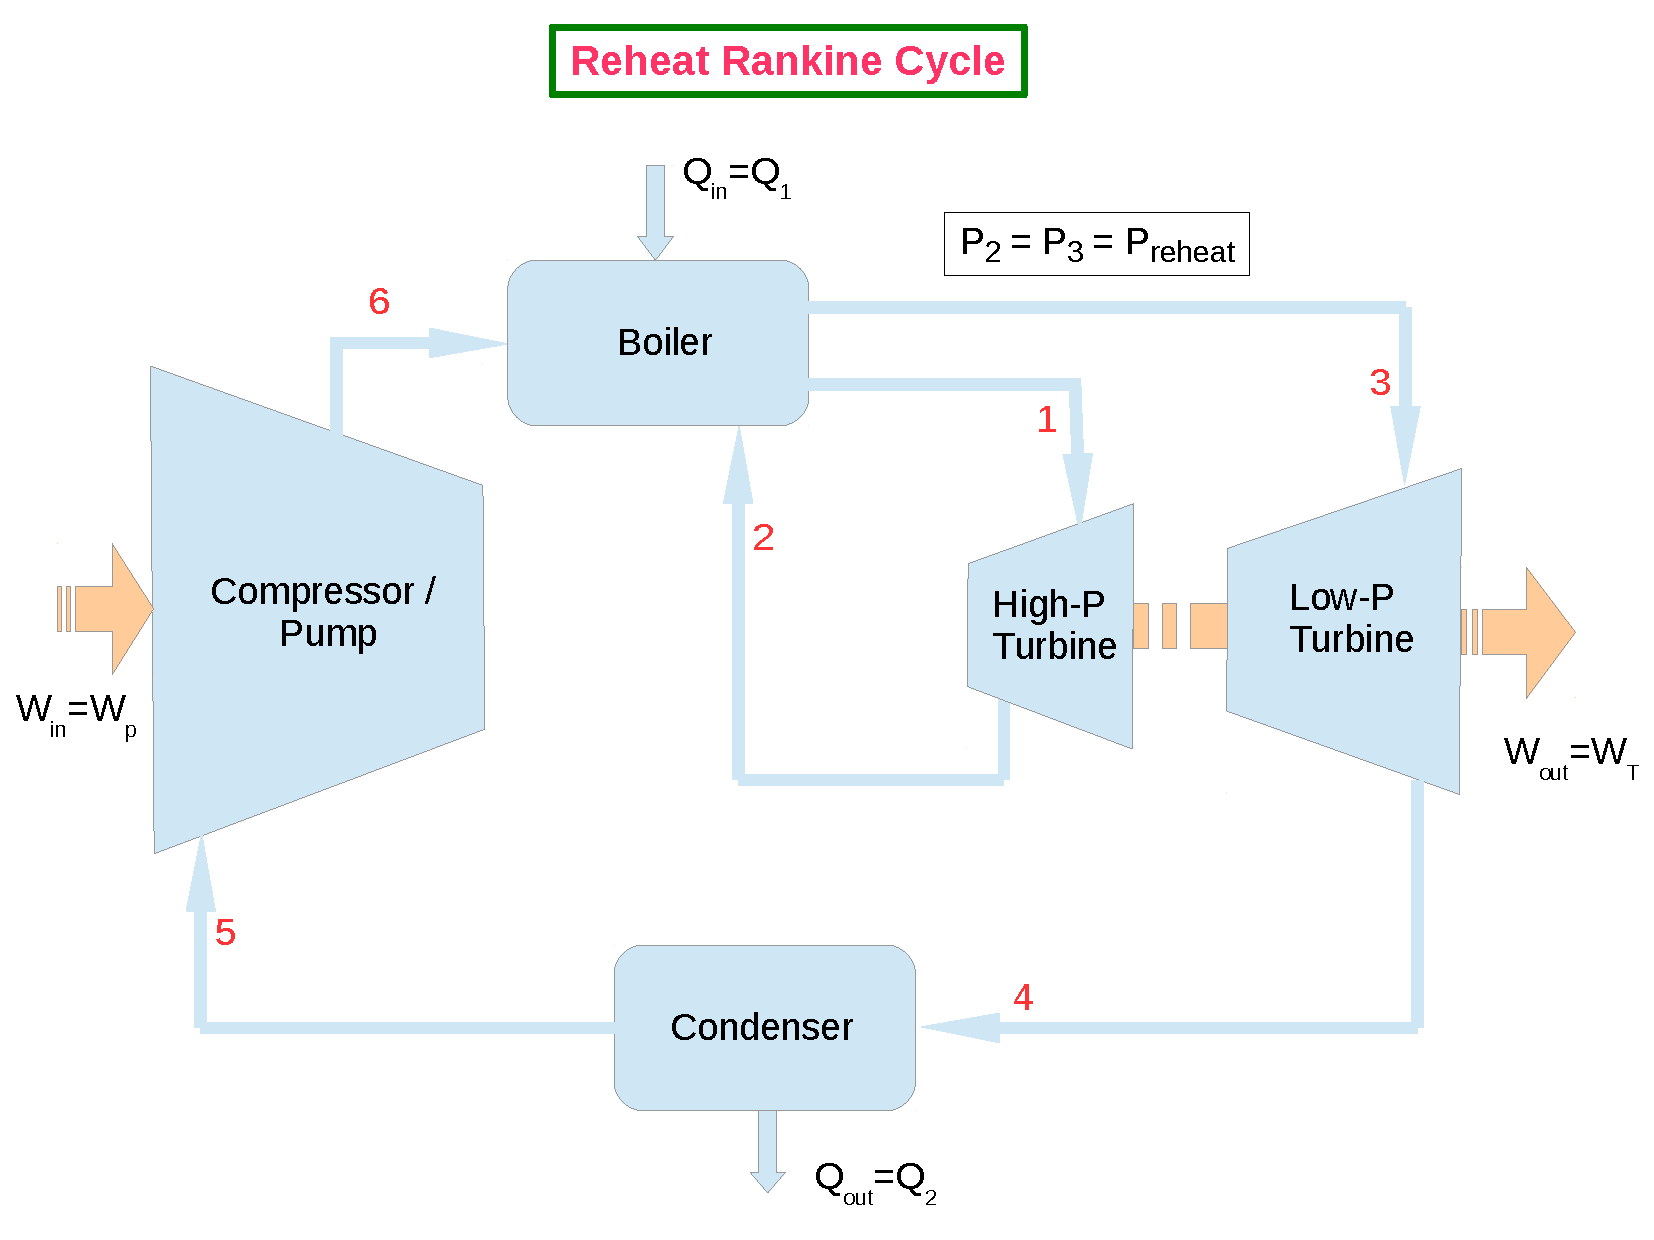
\includegraphics[width=6.25cm,clip]{./Pics/Reheat_Rankine_Cycle22}
           \end{center}
        \end{figure}} 
        \begin{enumerate}[(a)]\scriptsize\setcounter{enumi}{5}
           \item<5-> Disadvantages of Reheating:
              \begin{enumerate}[(i)]\scriptsize
                 \item<5->Reheating requires more maintenance;
                 \item<5->Enhancement of thermal efficiency may not be enough to match the larger costs associated with reheating the steam.
              \end{enumerate}
        \end{enumerate}
     \end{column}
  \end{columns}
 \normalsize
\end{frame}


%%%
%%% Slide
%%%
\begin{frame}
 \frametitle{Ideal Reheat Rankine Cycle}
  \begin{columns}
     \begin{column}[c]{0.5\linewidth} 
       \begin{center}
          \begin{figure}
             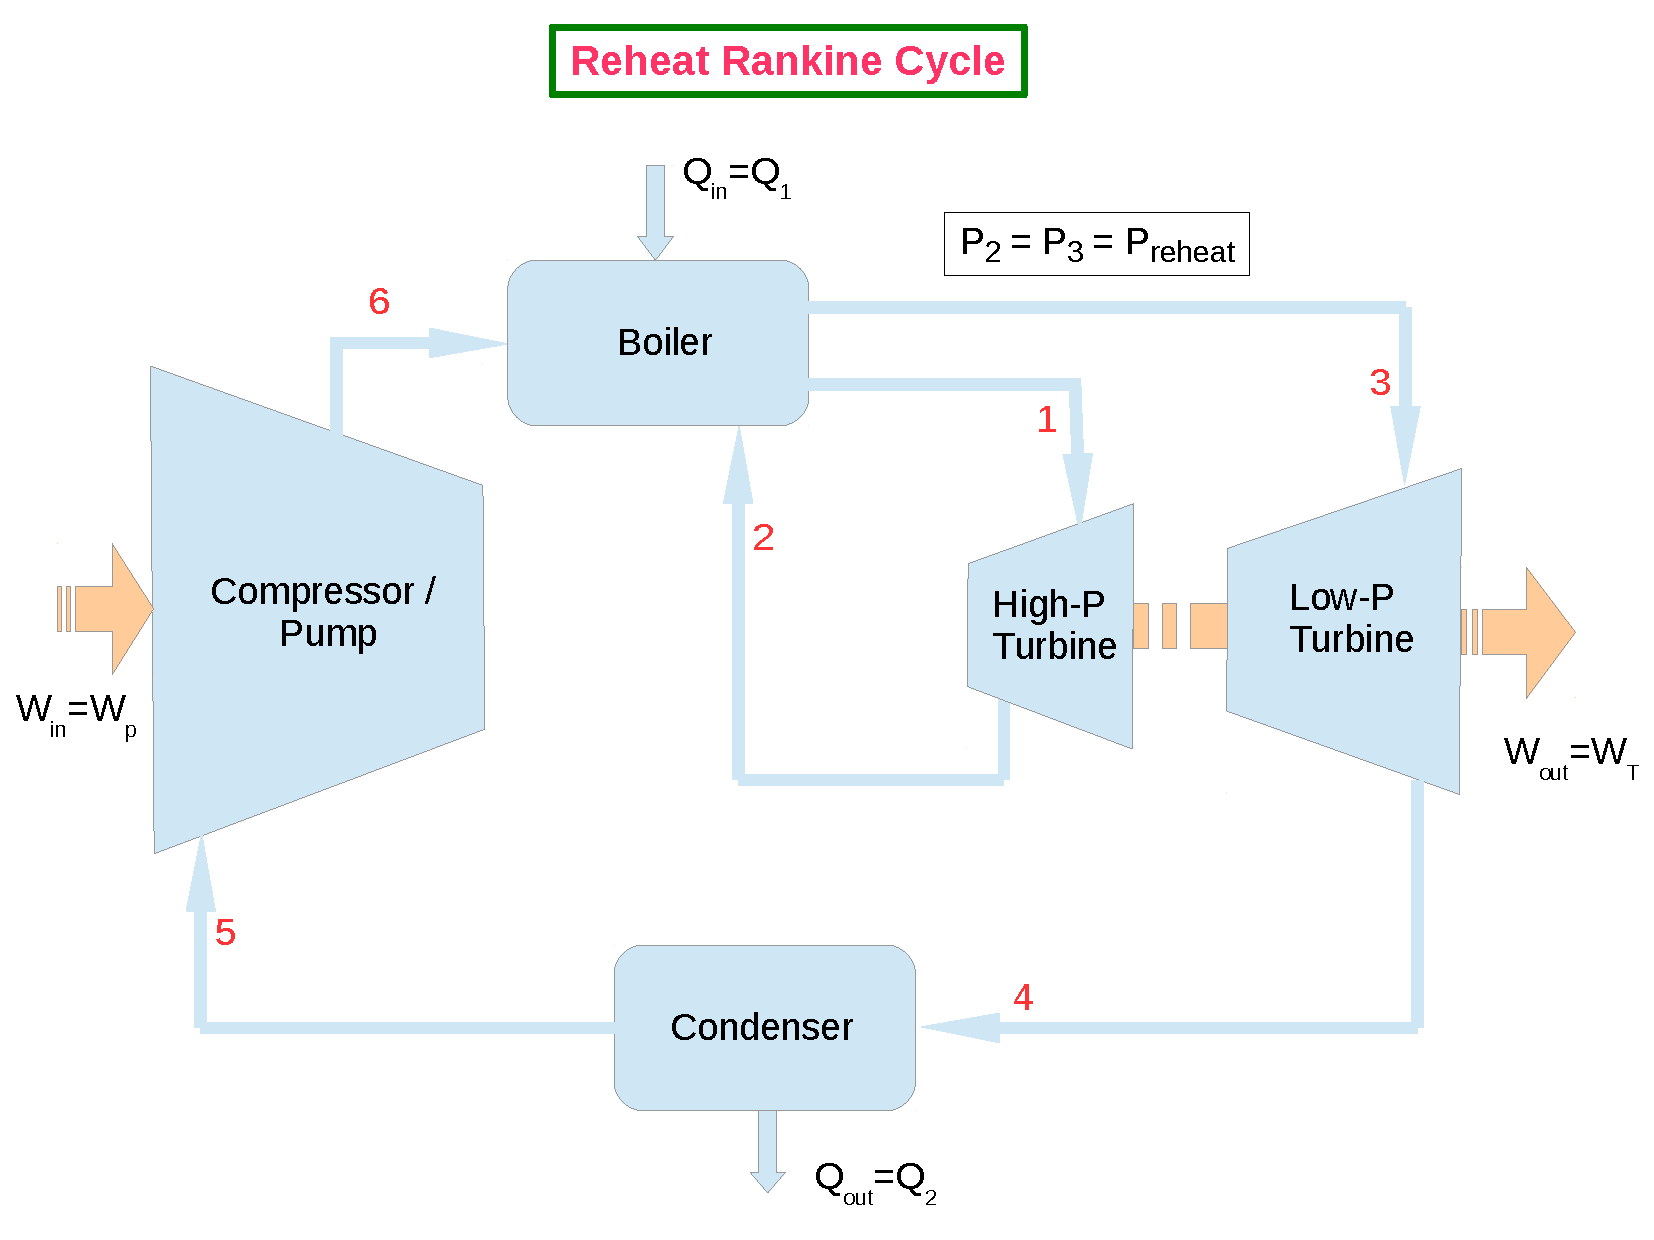
\includegraphics[width=6.25cm,clip]{./Pics/Reheat_Rankine_Cycle22}
          \end{figure}
       \end{center}
       \begin{enumerate}[(a)] \scriptsize\setcounter{enumi}{6}
          \item<1-> Total heat input: 
              \visible<1->{\begin{eqnarray}
                  \blue{Q_{\text{total}}}&=& Q_{\text{primary}} + Q_{\text{reheat}} \nonumber \\
                                    &=& \blue{\left(h_{1}-h_{6}\right)+\left(h_{3}-h_{2}\right)}
              \end{eqnarray}}
       \end{enumerate}
     \end{column}
     \begin{column}[c]{0.5\linewidth}
       \begin{center}
          \begin{figure}
             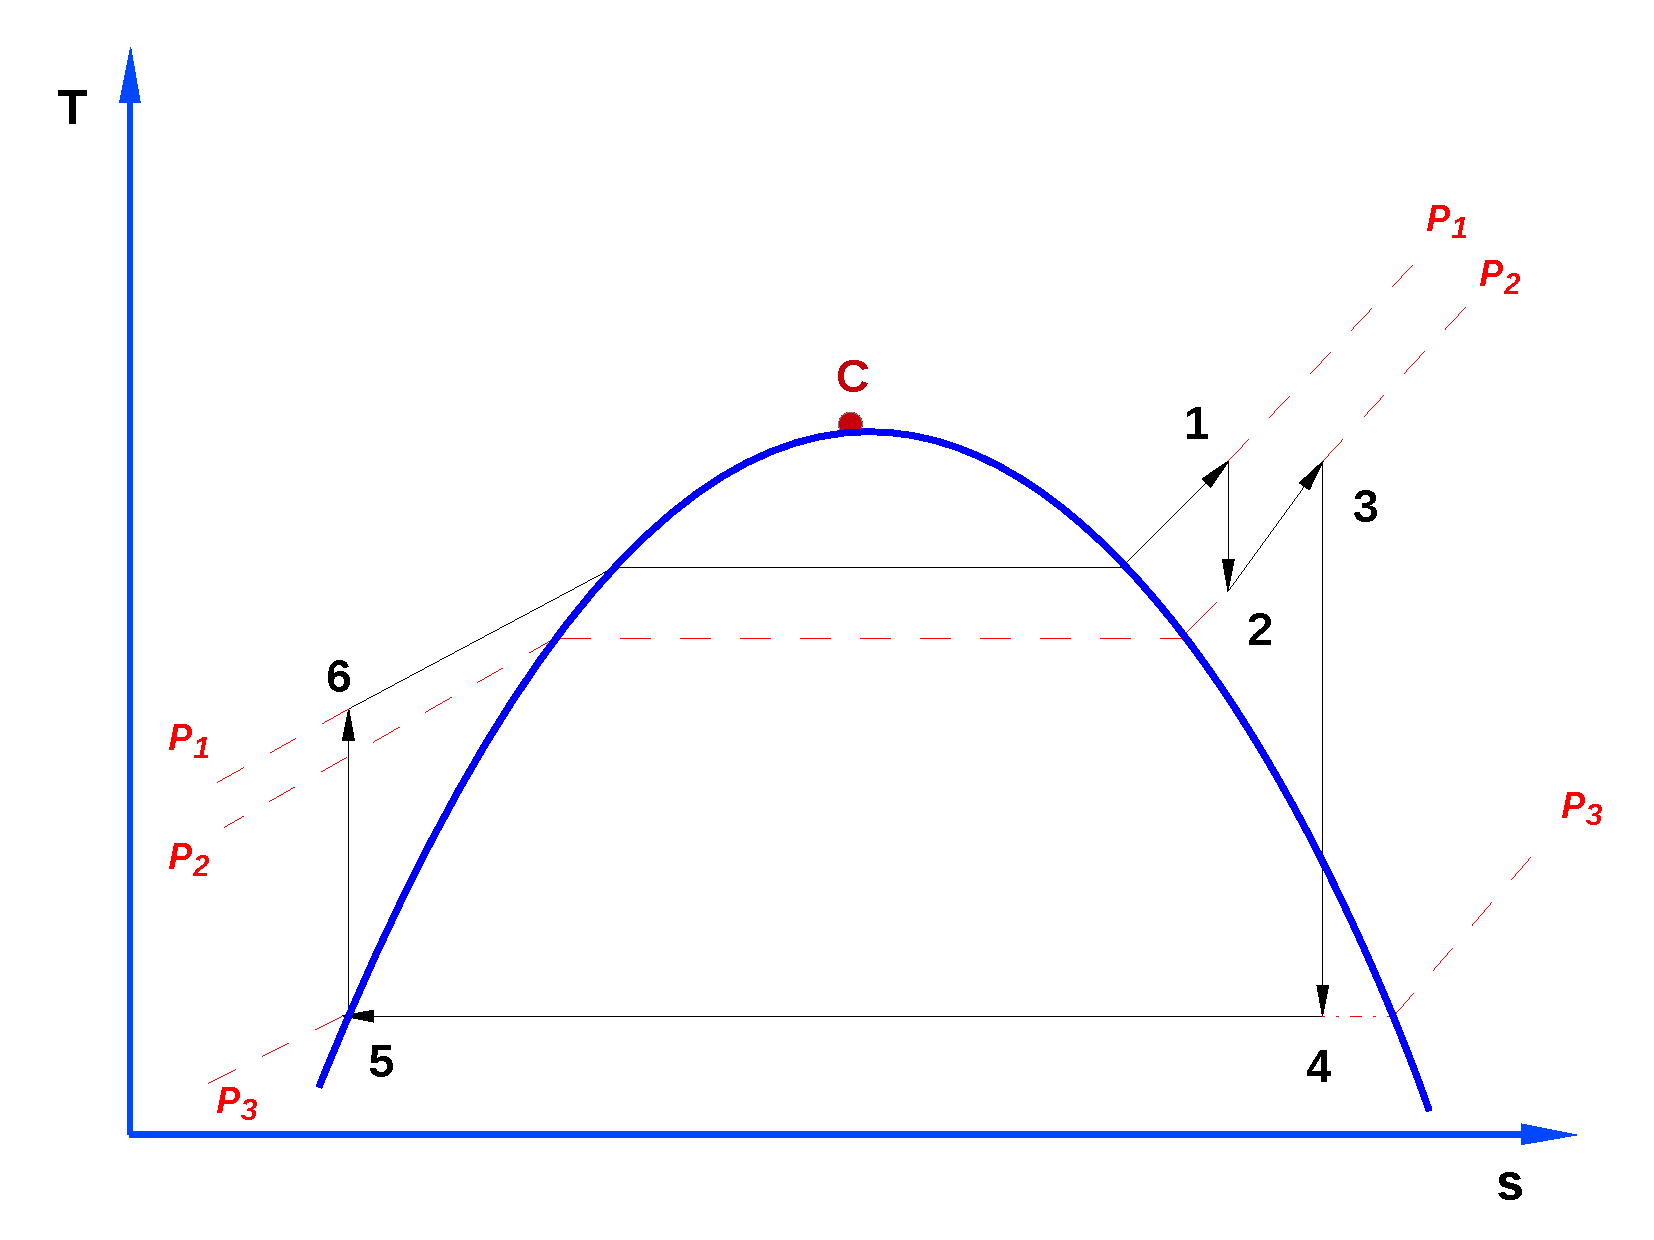
\includegraphics[width=6.25cm,clip]{./Pics/Reheat_Rankine_Cycle_Diagram2}
          \end{figure}
       \end{center}
       \begin{enumerate}[(a)] \scriptsize\setcounter{enumi}{7}
          \item<2-> Total turbine work output:
              \visible<2->{\begin{eqnarray}
                  \blue{W_{\text{turbine}}^{\text{total}}} &=& W_{\text{turbine}}^{\text{high-P}} + W_{\text{turbine}}^{\text{low-P}} \nonumber \\
                                                      &=& \blue{\left(h_{2}-h_{1}\right)+\left(h_{4}-h_{3}\right)}
              \end{eqnarray}}
       \end{enumerate}
     \end{column}
  \end{columns}
 \normalsize
\end{frame}


%%%% COMMENT
\begin{comment}

%%%
%%% Slide
%%%
\begin{frame}
 \frametitle{Ideal Regenerative Rankine Cycle (Open feedwater heater)}
  \begin{columns}
    \begin{column}[c]{0.5\linewidth}
      \begin{enumerate}[(a)]\scriptsize
         \item<1-> In simple RC the \blue{temperature of the working fluid entering the boiler is substantially lower than the boiler steam exiting temperature}.  This results in \red{lower thermal efficiency};
         \item<2-> In the \blue{Regenerative Rankine Cycle} the temperature of the fluid leaving the pump ({\it feedwater}) is raised in several stages using steam extracted from the turbine;
         \item<3-> The device where the feedwater is heated by regeneration is called a \blue{regenerator} or \blue{feedwater heater (FWH)};
     %\item <4-> Not only improve thermal efficiency but also deaerates the feedwater that helps prevent corrosion and pump cavitation;
         \item<4-> A FWH is a heat exchanger where heat is transferred from the steam to the feedwater either by mixing the two fluid streams (\blue{open feedwater heaters}) or without mixing them (\blue{closed feedwater heaters}).
    \end{enumerate} 
   \end{column}
   \begin{column}[c]{0.5\linewidth} 
     \begin{center}
        \begin{figure}
            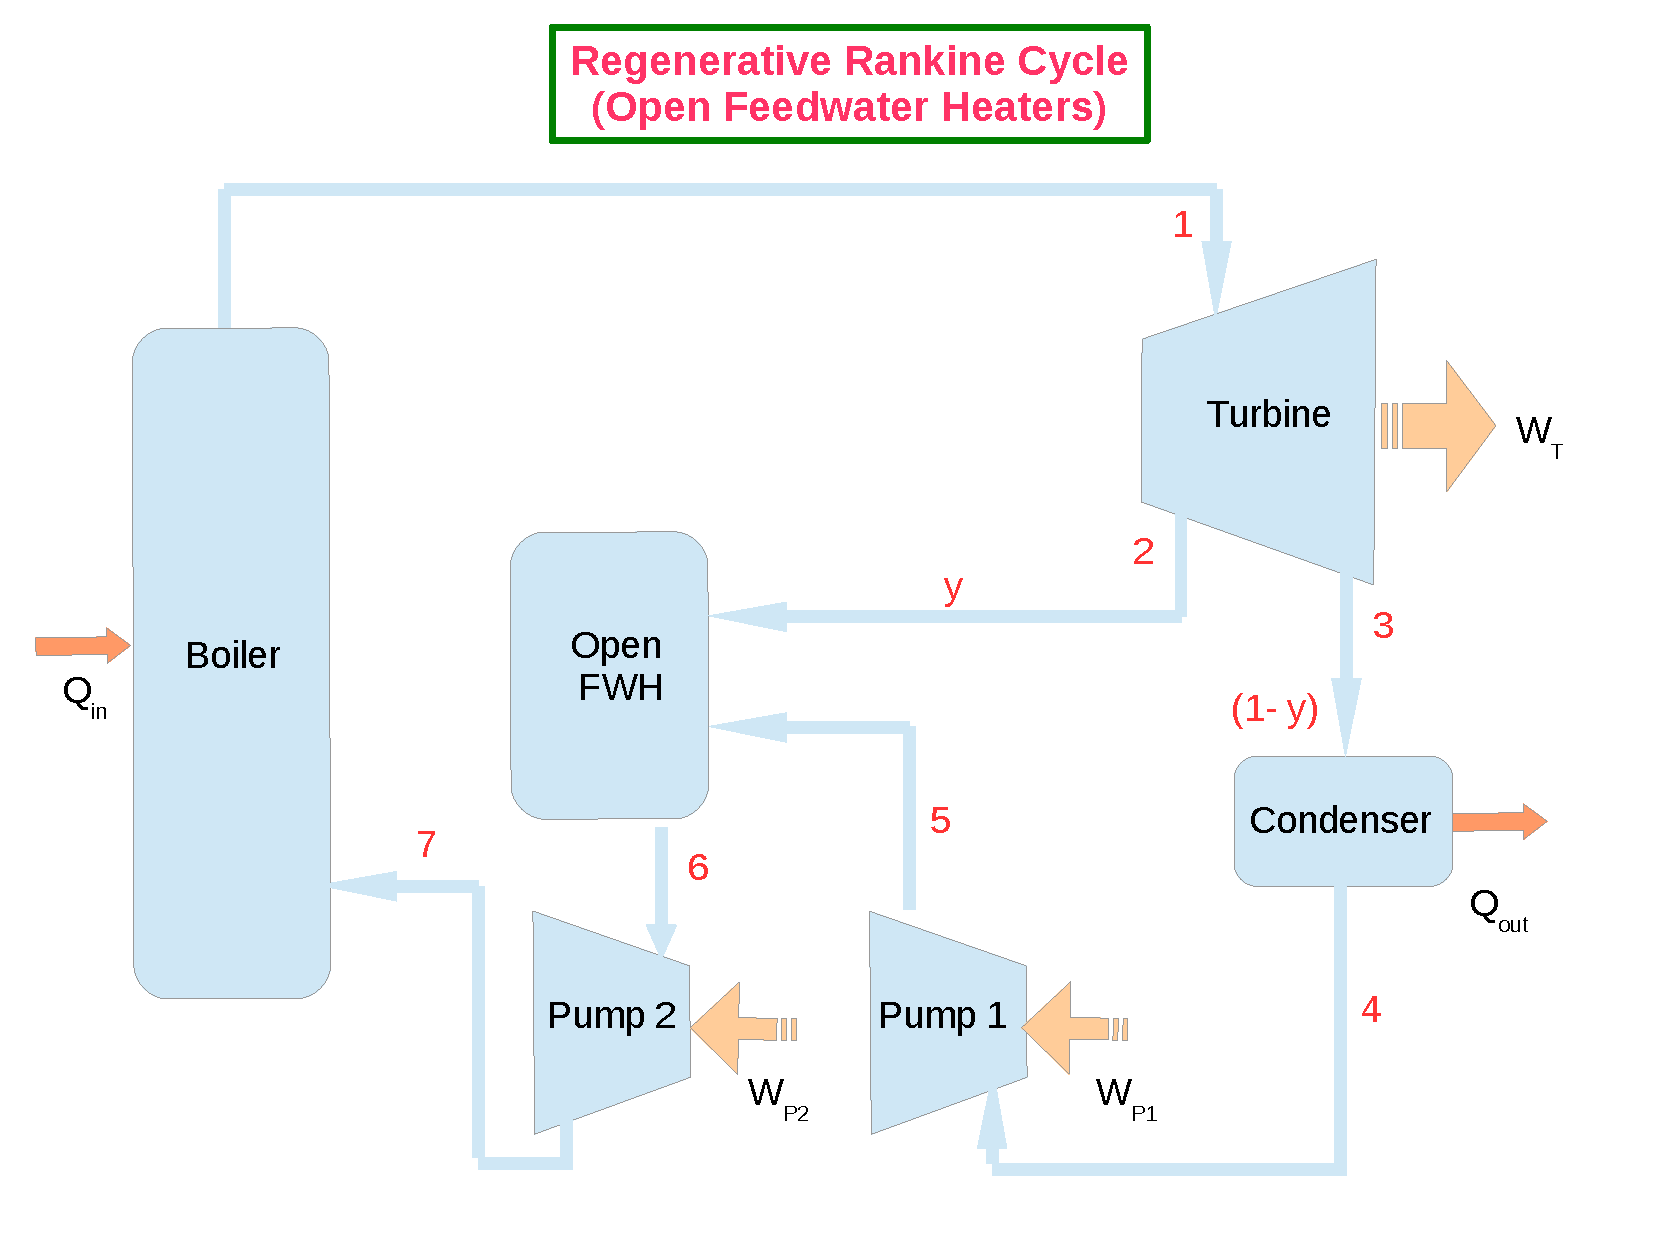
\includegraphics[width=6.5cm,clip]{./Pics/RegenerativeOpen_RankineCycle}
        \end{figure}
     \end{center}
   \end{column}
  \end{columns}
 \normalsize
\end{frame}


%%%
%%% Slide
%%%
\begin{frame}
 \frametitle{Ideal Regenerative Rankine Cycle (Open feedwater heater)}
  \begin{columns}
    \begin{column}[c]{0.5\linewidth}
     \begin{center}
        \begin{figure}
            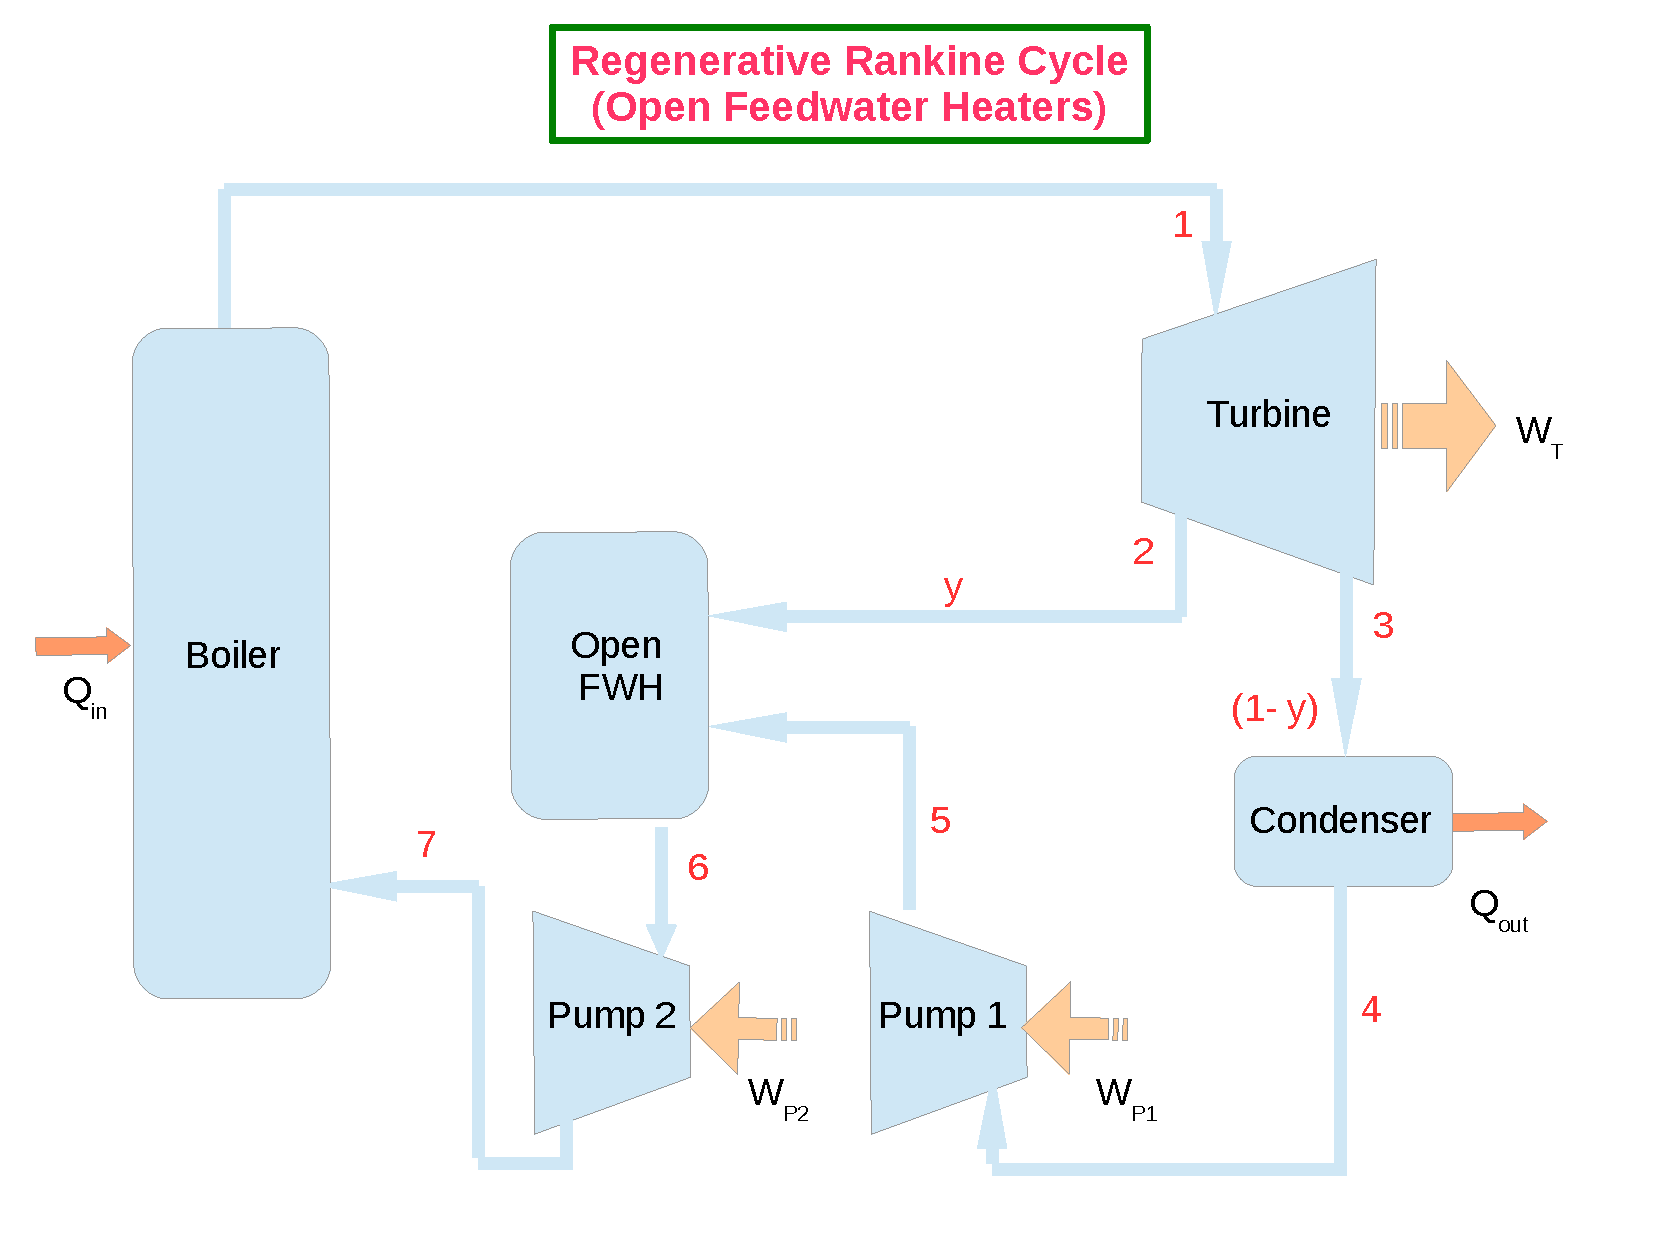
\includegraphics[width=5.5cm,clip]{./Pics/RegenerativeOpen_RankineCycle}
        \end{figure}
     \end{center}
     \begin{enumerate}[(a)]\setcounter{enumi}{4}\scriptsize
         \item<1->  A fraction of the steam extracted from the turbine \blue{($y$)} leaves the FWH as {\it saturated liquid} $\left(P_{\text{FWH}}\right)$, and a second pump raises the pressure to $P_{\text{boiler}}$;
         \item<2-> Heat balance in the cycle:
             \visible<2->{\begin{eqnarray}
                && \blue{Q_{\text{in}} = h_{1}-h_{7}} \\
                && \blue{Q_{\text{out}} = \left(1 - y \right)\left(h_{4} - h_{3}\right)} 
             \end{eqnarray}}
     \end{enumerate}
   \end{column}
    \begin{column}[c]{0.5\linewidth}
     \begin{center}
        \begin{figure}
            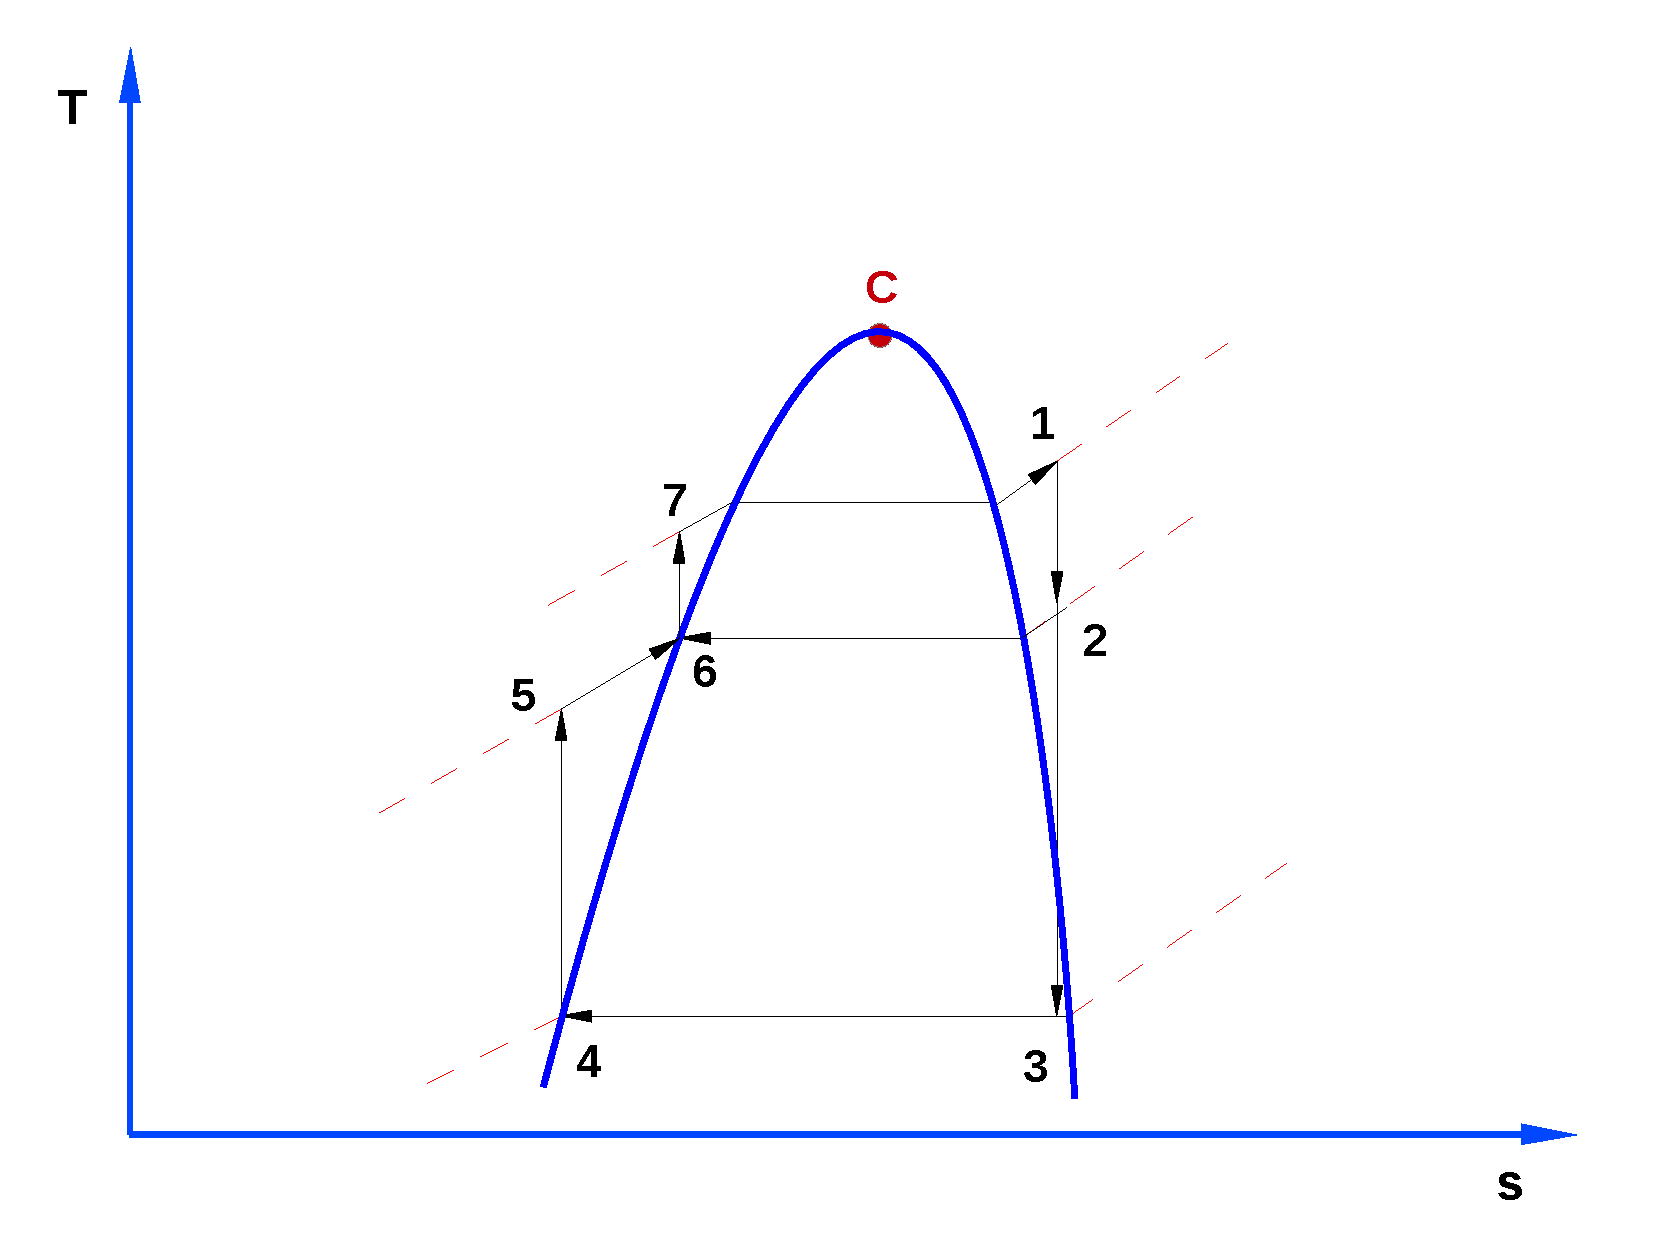
\includegraphics[width=6.cm,clip]{./Pics/RegenerativeOpen_RankineCycle_Diagram}
        \end{figure}
     \end{center}
     \begin{enumerate}[(a)]\setcounter{enumi}{6}\scriptsize
         \item<3-> Pump and turbine work:
             \visible<3->{\begin{eqnarray}
                \blue{W_{\text{Turbine}}^{\text{out}} = \left[y h_{2} + \left(1-y\right)h_{3}\right]-h_{1}}\\ 
                \blue{W_{\text{Pump}}^{\text{in}} = \left(1 - y \right) W_{\text{Pump,1}}^{\text{in}} + W_{\text{Pump,2}}^{\text{in}}}
             \end{eqnarray}}
     \end{enumerate}
   \end{column}
  \end{columns}
 \normalsize
\end{frame}

%%%
%%% Slide
%%%
\begin{frame}
 \frametitle{Ideal Regenerative Rankine Cycle (Closed feedwater heater)}
  \begin{columns}
    \begin{column}[c]{0.5\linewidth}
     \begin{center}
        \begin{figure}
            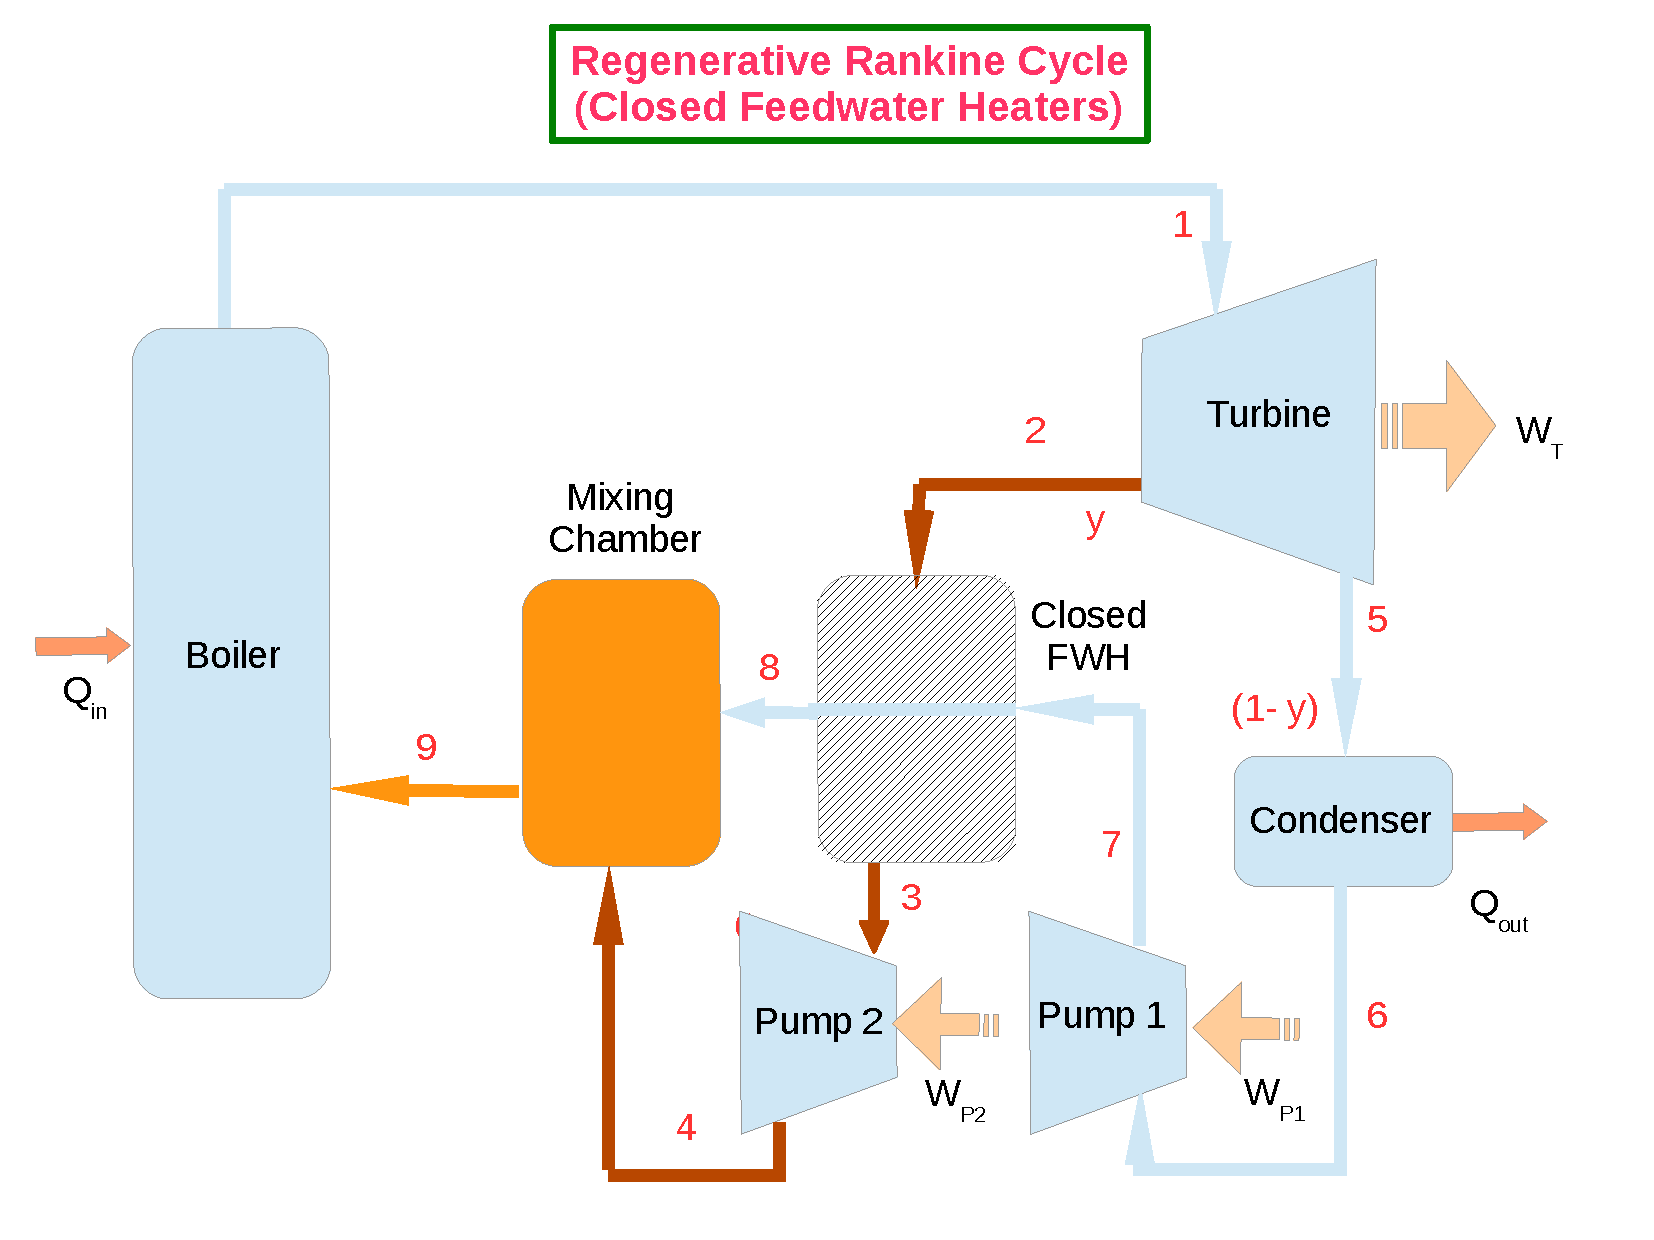
\includegraphics[width=6.cm,clip]{./Pics/RegenerativeClosed_RankineCycle}
        \end{figure}
     \end{center}
   \end{column}
    \begin{column}[c]{0.5\linewidth}
     \begin{center}
        \begin{figure}
            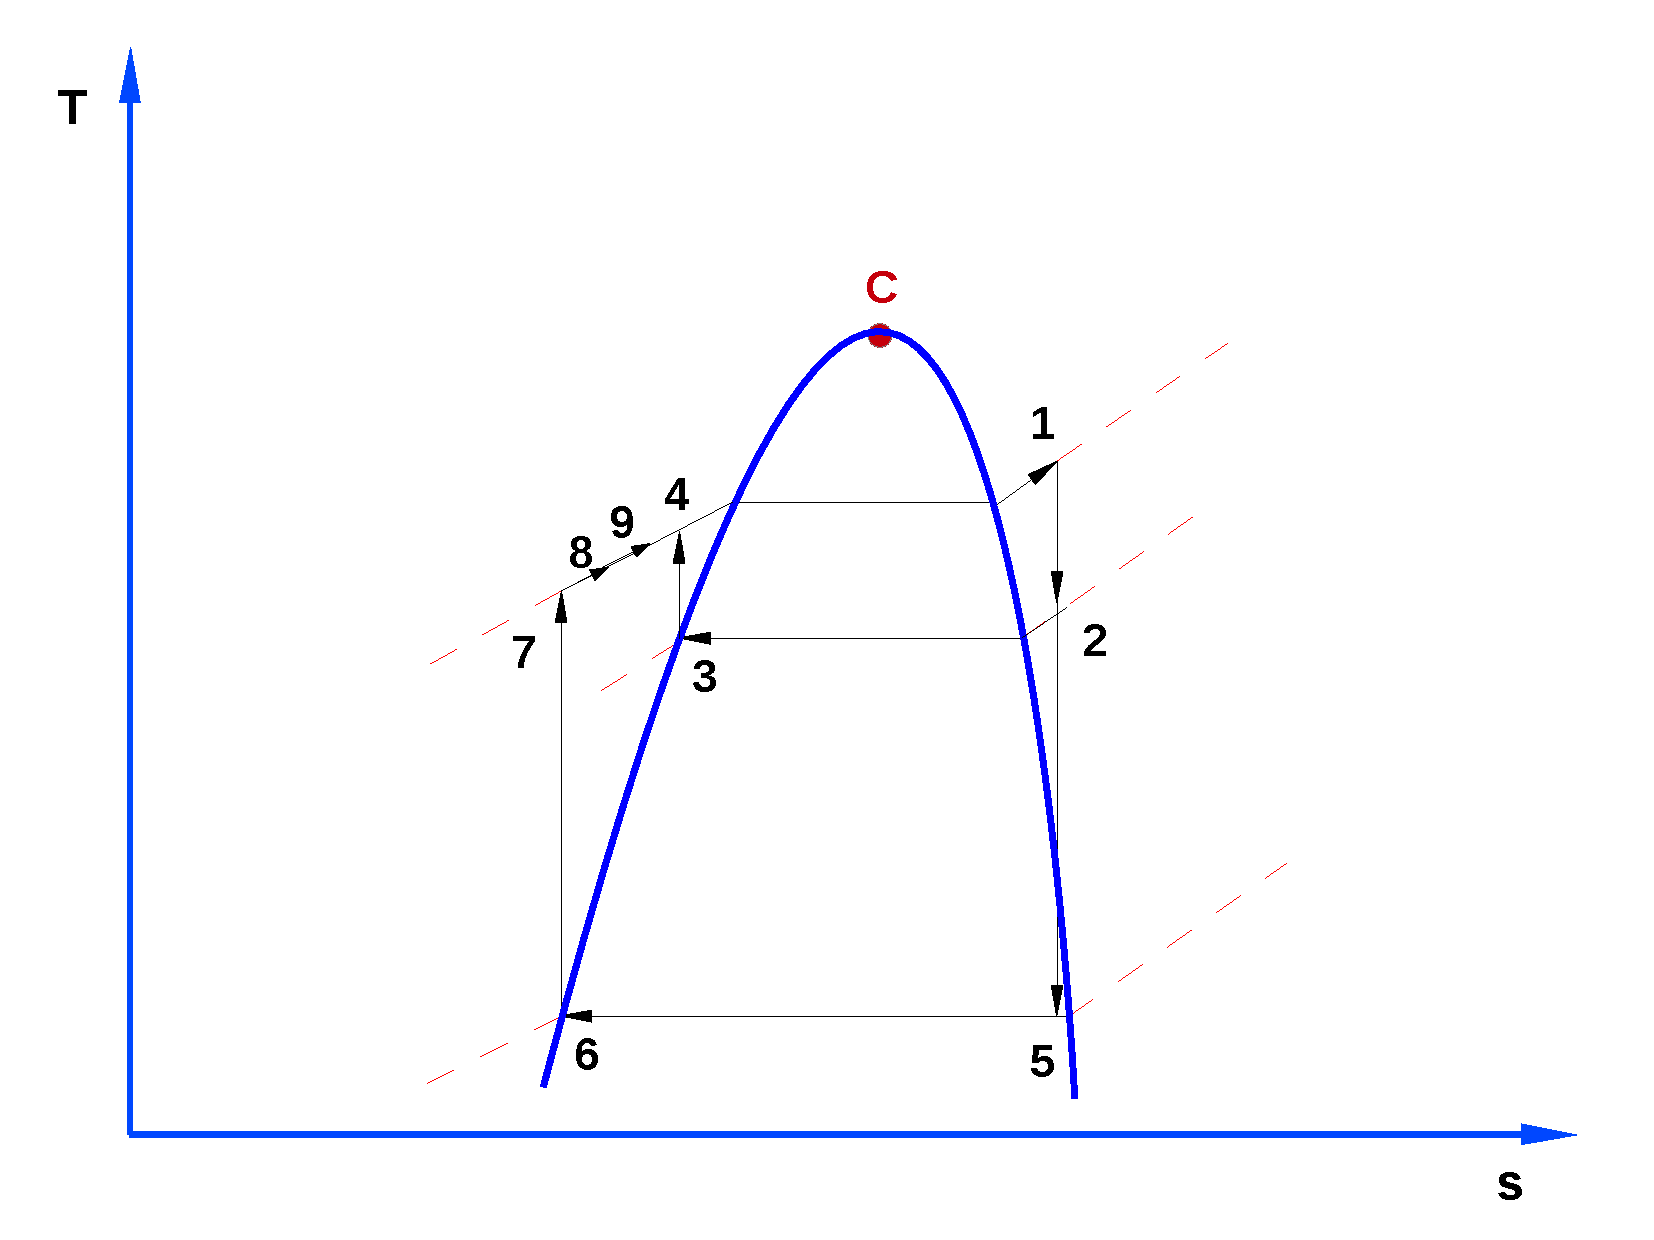
\includegraphics[width=6.25cm,clip]{./Pics/RegenerativeClosed_RankineCycle_Diagram}
        \end{figure}
     \end{center}
   \end{column}
  \end{columns}
 \normalsize
\end{frame}


%%%
%%% Slide
%%%
\begin{frame}
 \frametitle{Regenerative $\times$ Simple Rankine Cycles}
  \begin{columns}
   \begin{column}[c]{0.5\linewidth}
    \begin{enumerate}[(a)]
     \item<1-> Advantages of Regenerative cycle over Simple Rankine Cycle
     \begin{enumerate} [(i)]%\scriptsize
      \item<1-> The heating process in the boiler tends to become reversible;
      \item<1-> Thermal stresses in boiler are minimised due to the smaller temperature ranges in the boiler;
      \item<1-> Thermal efficiency is improved as the average temperature of heat addition to the cycle is increased;
      \item<1-> Due to continuous steam extraction, the content of moisture is reduced and this decreases the corrosion in the turbine;
      \item<1-> The size of the condenser is smaller (lower cost and better maintenance).
     \end{enumerate}
    \end{enumerate} 
   \end{column}
%
   \begin{column}[c]{0.5\linewidth}  
    \begin{enumerate}[(a)]\setcounter{enumi}{1}
     \item<2-> Disadvantages of Regenerative cycle over Simple Rankine Cycle
     \begin{enumerate}[(i)] %\scriptsize
      \item<2-> Design of the power plant is more complex;
      \item<2-> As the number of heaters is increased, the greater maintenance (larger cost) is required;
      \item<2-> Heater are usually costly and the gain in thermal efficiency may not be enough. 
     \end{enumerate}
    \end{enumerate} 
   \end{column}
  \end{columns}
  
\end{frame}
 
\end{comment}
%%%
%%% Slide
%%%
\begin{frame}
 \frametitle{Example 3: Reheat Rankine Cycle}
    \scriptsize In the secondary cooling circuit of a nuclear power plant, the steam generator (boiler / reheater) produces superheated steam (SHS) and is connected to two turbines operating as a reheat Rankine cycle. Isentropic efficiencies of the first $\left(\eta_{\text{T1}}\right)$ and second $\left(\eta_{\text{T2}}\right)$ turbines are 84$\%$ and 80$\%$, respectively. (a) Determine {\it (a)-(t)} in the table below. Calculate the (b) power produced by the turbines, (c) heat supplied by the boiler and (d) heat extracted from the condenser. (e) Sketch the $Ts$ diagram of the cycle. Assume that the heat capacity at constant pressure $\left(\text{C}_{\text{p}}\right)$ is 4.18 $\frac{\text{kJ}}{\text{kg.}^{\circ}\text{C}}$.

       \begin{center}
         \begin{tabular}{c | c c c c c c  }
           \hline\scriptsize
           {\bf Stage} & $P$    & $T$             &  State       & Quality     & $h$                 & $s$                      \\
                       & (bar)  & ($^{\circ}$C)    &              &             & (kJ.kg$^{-1}$)       & (kJ.(kg.K)$^{-1}$)        \\
           \hline
            {\bf 1 }   & 40         & 320         & SHS          & --          & {\bf (a)}           & {\bf (b)}                 \\
            {\bf 2 }   &  --        & {\bf (c)}   & {\bf (d)}    & {\bf (e)}   & {\bf (f)}           & {\bf (g)}          \\
            {\bf 3 }   & 7          & 370         & SHS          & --          & {\bf (h)}           & {\bf (i)}                 \\
            {\bf 4 }   & 0.10       & {\bf (j)}   & {\bf (k)}    & {\bf (l)}   & {\bf (m)}           & {\bf (n)}                     \\
            {\bf 5 }   & 0.10       & {\bf (o)}   & {\bf (p)}    & --          & {\bf (q)}           & {\bf (r)}    \\
            {\bf 6 }   & 40         & --          & {\bf (s)}    & --          & {\bf (t)}           & --                      \\
           \hline
         \end{tabular}
        \end{center}
         \begin{center}
            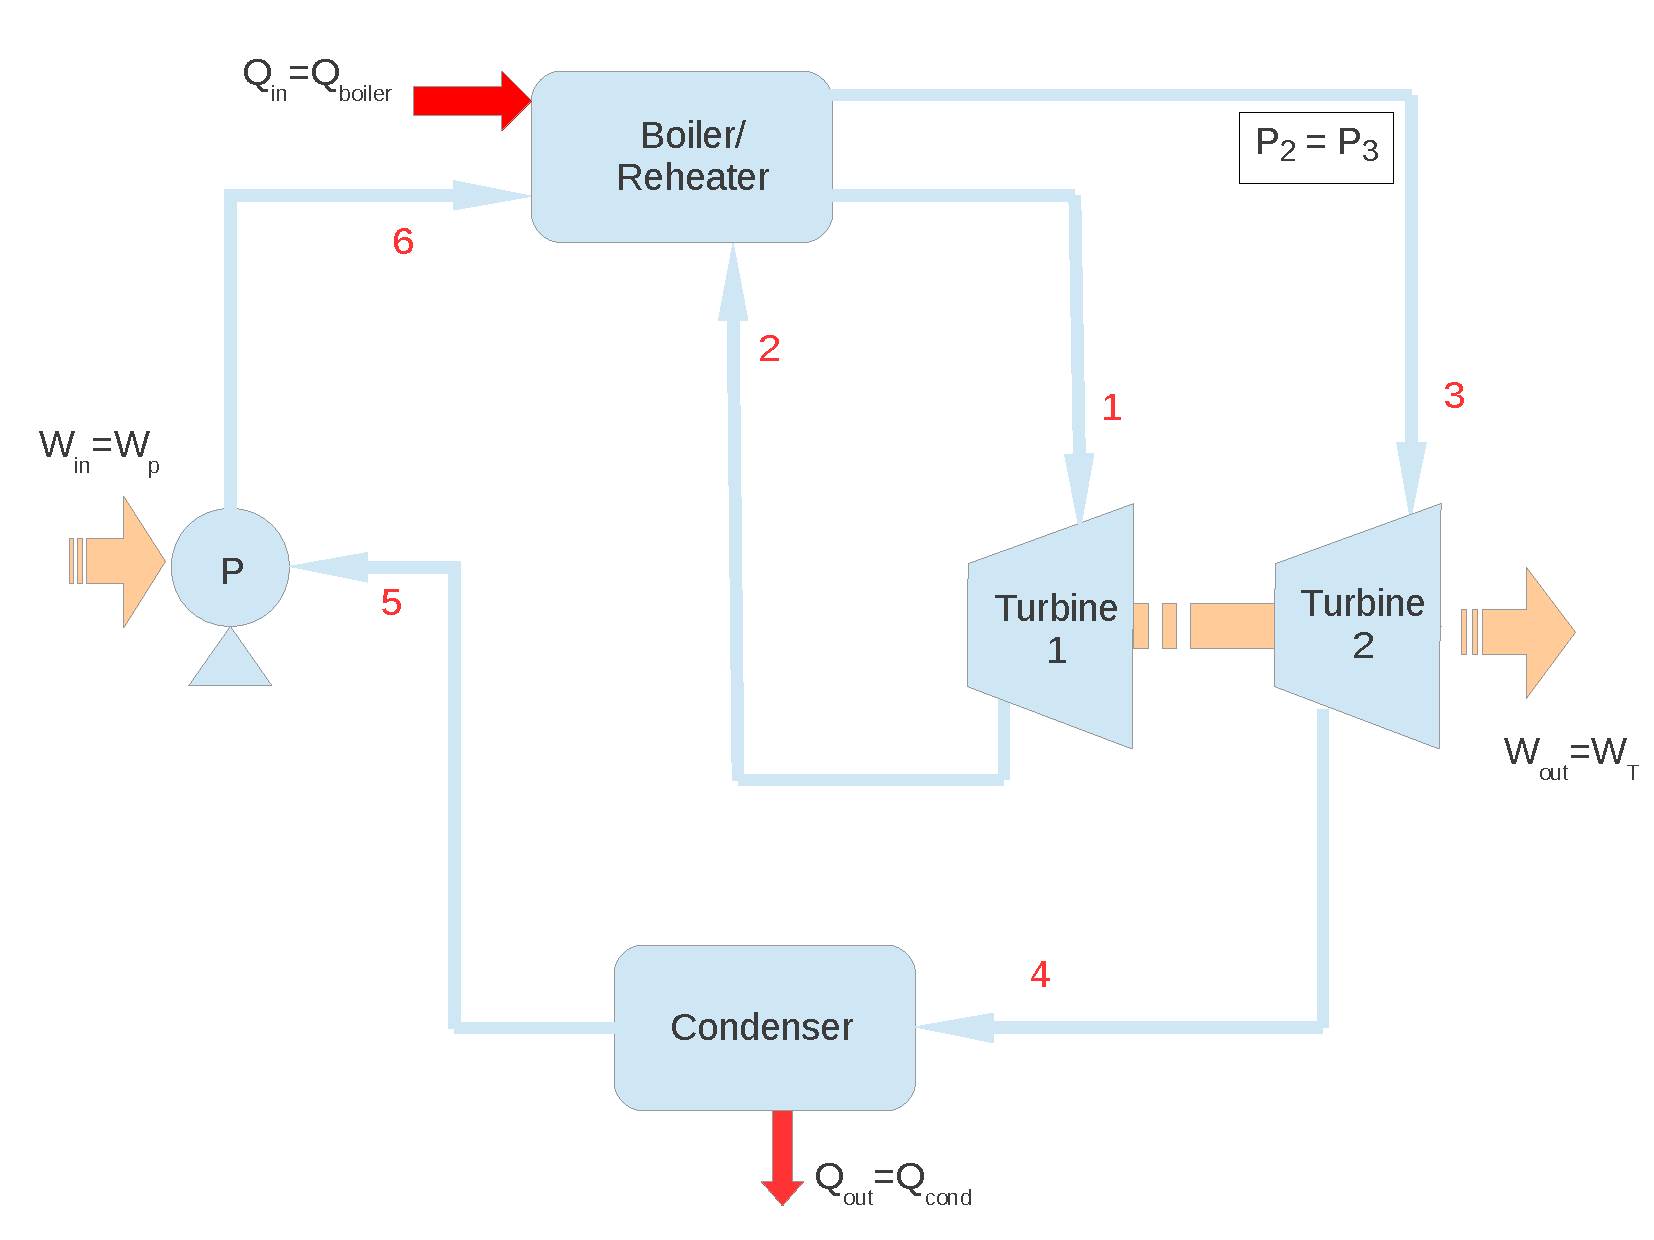
\includegraphics[width=4.5cm,clip]{./Pics/Exam_Reheat_Rankine_Cycle}
         \end{center}
%       \end{column}
%       \begin{column}[c]{0.5\linewidth} 
%kklkl
%       \end{column}
%    \end{columns}

\end{frame} 



%%%           %%%
%%%  SECTION  %%% 
%%%           %%%
\section{Refrigeration Systems}

%%%% SUBSECTION
\subsection{Introduction}

%%%
%%% Slide
%%%
\begin{frame}
 \frametitle{Overview}
  \begin{columns}
   \begin{column}[c]{0.45\linewidth}
    \begin{enumerate}[(a)] 
     \item <1-> When a heat engine is thermodynamically \underline{reversed}, the \textcolor{blue}{directions of all the energy flows are reversed};
     \item <2-> Work input ({\it W}) causes thermal energy transfers $Q_{2}$ from the cold reservoir and $Q_{1}=Q_{2}+W$ to the hot reservoir; 
     \item <3-> Such reversed process can not however occur spontaneously. The transfer of heat from a cold reservoir to a hot reservoir requires special devices called \textcolor{blue}{refrigerators}.
    \end{enumerate}
   \end{column}
   \begin{column}[c]{0.55\linewidth}
    \begin{figure}%
     \begin{center}
      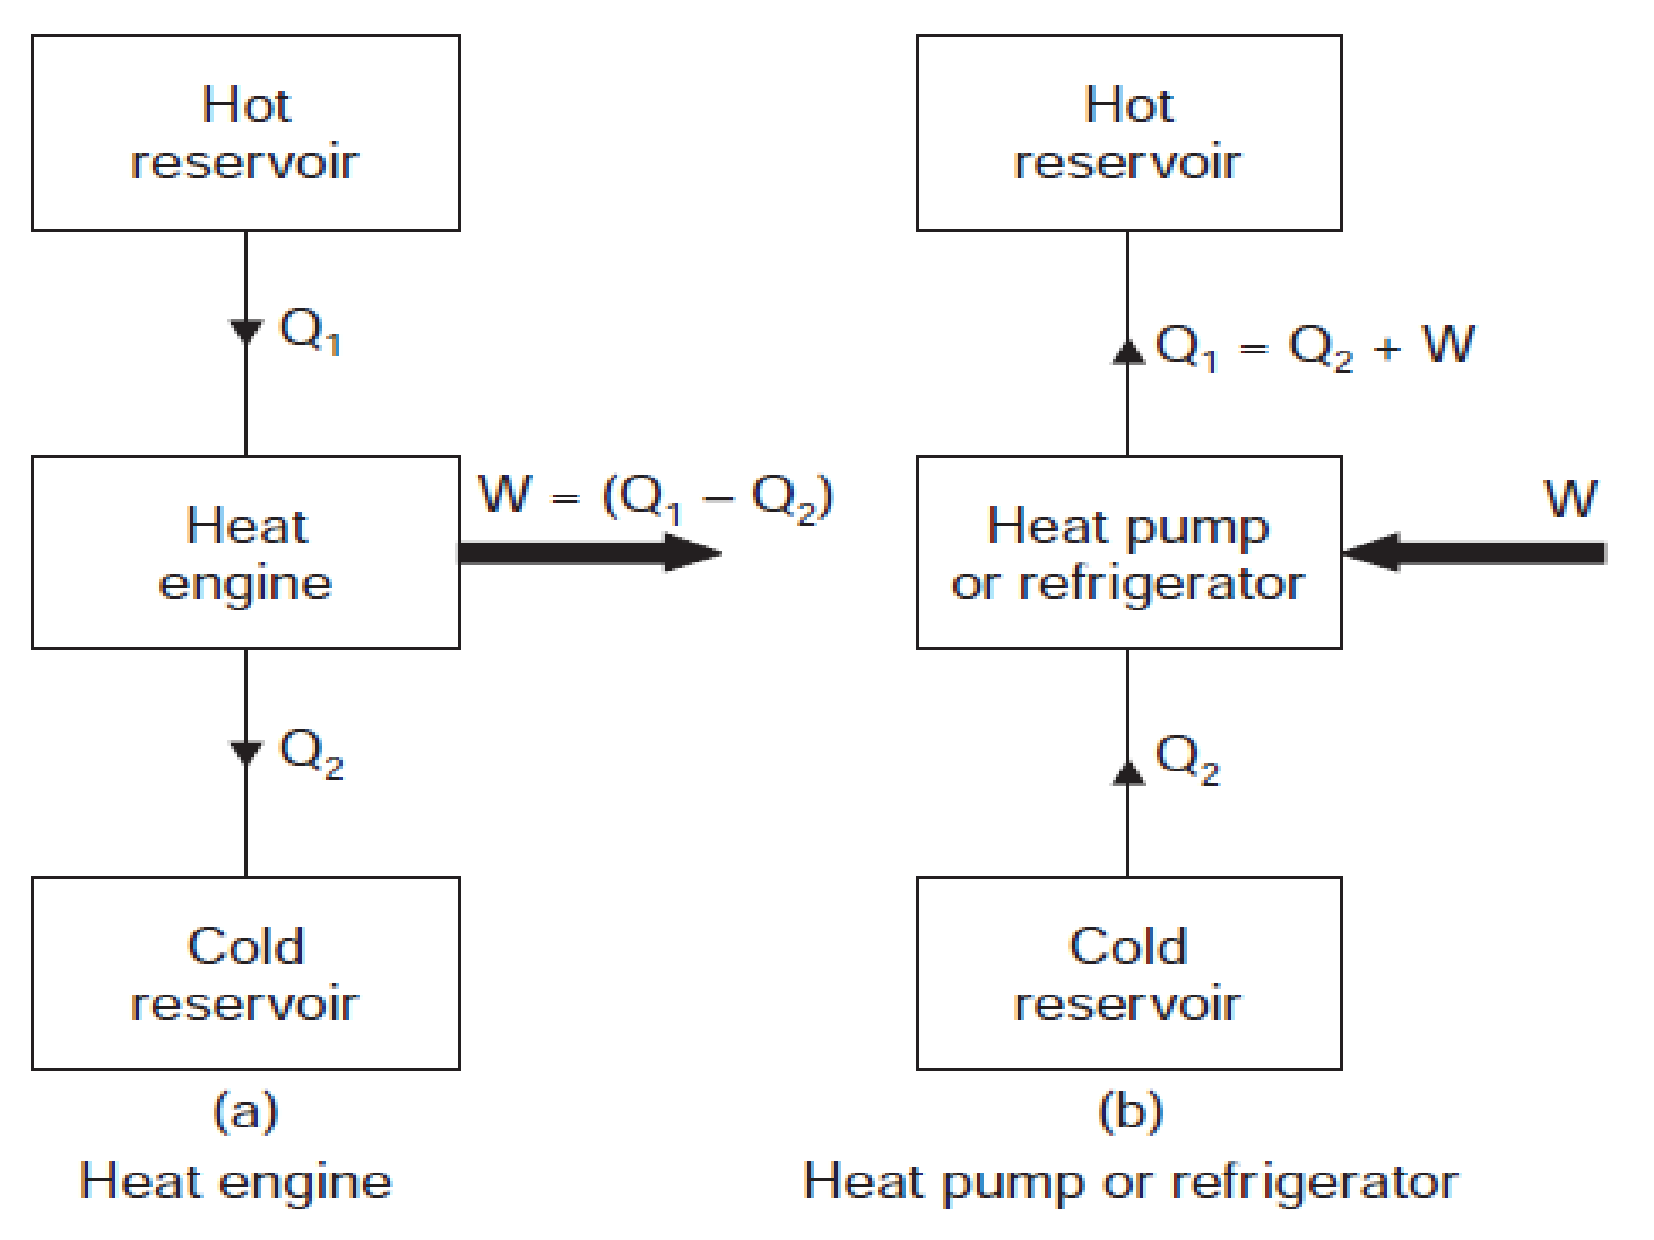
\includegraphics[width=6.5cm,clip]{./Pics/Overview_Refrig1}
     \end{center}
    \end{figure}  
   \end{column}  
  \end{columns}
\end{frame}

%%%% COMMENT
\begin{comment}

%%%
%%% Slide
%%%
\begin{frame}
 \frametitle{Classification of Refrigerants}
 \begin{enumerate}[1]\scriptsize
   \item <1-> \textcolor{blue}{Refrigerant} is the working fluid used in refrigeration equipment; 
   \item <2-> Its main function is to \textcolor{blue}{carry/reject heat} as:
     \begin{enumerate}[(a)]\scriptsize
        \item<2-> \blue{sensible heat}, i.e., heat transfer with change in temperature or;
        \item<2-> \blue{latent heat}, i.e., heat transfer with no change in temperature (during phase change);
     \end{enumerate}
   \item <3-> In other words, refrigerant fluids act as cooling agents by absorbing heat from a body or substance;
   \item <4-> \textcolor{blue}{Primary Refrigerants} (PR) are directly involved in refrigeration systems and is usually followed by a \textcolor{blue}{phase change}. The cycle encompass compression, condensation, expansion and evaporation;
   \item <5-> \textcolor{blue}{Secondary Refrigerants} (SR) is used as a heat transfer medium \textcolor{blue}{without phase change} but \textcolor{blue}{with change in temperature};
   \item <6-> As an example, in a conventional air conditioning system, there are 2 cycles: 
    \begin{enumerate}[(a)]\scriptsize
     \item <7-> \textcolor{blue}{Water} is the \textcolor{blue}{{\it primary refrigerant}} that circulates throughout the closed-loop cycle involving evaporator, compressor, condenser and expansion valve, whereas;
     \item <8-> \textcolor{blue}{Air} is the \textcolor{blue}{{\it secondary refrigerant}}.
    \end{enumerate}
    \item <9-> \visible<9->{PR are used in vapour-compression systems} \visible<10->{whereas SR are liquids used for transporting low-temperature heat energy.}
  \end{enumerate}
\end{frame}


%%%
%%% Slide
%%%
\begin{frame}
 \frametitle{Classification of Refrigerants}
%\textcolor{blue}{\bf PR} can be further classified into 4 categories depending upon their characteristics: 
 \begin{enumerate}[1]\setcounter{enumi}{7}\scriptsize
   \item<1-> Primary Refrigerants (PR): 
     \begin{enumerate}[(a)]\scriptsize
       \item<1-> \textcolor{red}{Halocarbon Compounds:} contains 1 or more halogens {\it (Cl, F and Br)}. Commonly traded under the brand names of {\it Freon, Genetron etc} under the family of CFCs (chloro fluoro carbons) -- 1940-1990. Hydrogen has replaced chlorine and make this class of refrigerants more $\lq$environmental friendly' with a designation HFC (hydrofluiro carbons -- HFC). All halocarbon refrigerants are named as {\it R-XYZ}, e.g., {\it R-22} (monochloro difluoro-methane), {\it R-114} (dichloro tetrafluoro-ethane); 
       \item<1-> \textcolor{red}{Inorganic Compounds:} e.g., ammonia ({\it R-117}), CO$_{2}$ ({\it R-744}), SO$_{2}$ ({\it R-764}), water ({\it R-718}), etc;
       \item <1-> \textcolor{red}{Hydrocarbons} are often in the petroleum and petrochemical industry in liquefaction of gases, e.g., methane ({\it R-50}), propane ({\it R-290}), etc;
       \item <1-> \textcolor{red}{Azeotropes} are mixtures of 2 or more substances that behave as if they are compounds. This is because they can not be separated into their individual components by distillation. An azeotrope substance evaporates and condenses as a single substance with properties that are intrinsically different from the original constituents. E.g., {\it R-500}: 74$\%$ of {\it R-12} and 26$\%$ of {\it R-115}, etc;
       \item <1-> \textcolor{red}{Unsaturated Organic Compounds} are hydrocarbons based on ethylene and propylene, e.g., Trichloro ethylene ({\it R-1120}), Propylene ({\it R-1270}), etc.
     \end{enumerate}
   \item<2-> Secondary Refrigerants (SR): 
     \begin{enumerate}[(a)]\scriptsize
       \item <2-> SR are indirect refrigerants that transfer heat from the substance that need to be cooled to the evaporator; 
       \item <2-> Change in temperature are due to the absorption of heat followed by rejection in the evaporator with \textcolor{blue}{{\bf no} phase change};
       \item <2-> SR fluids commonly found in industrial and domestic applications are water, brine, anti-freezing (solution of water and ethylene glycol, propylene glycol, calcium chloride etc).
     \end{enumerate}
 \end{enumerate}
\end{frame}


%%%% COMMENT
\end{comment}
%%%
%%% Slide
%%%
\begin{frame}
 \frametitle{Refrigerator and Heat Pump}
  \begin{columns}
   \begin{column}[c]{0.45\linewidth}
    \begin{enumerate}[(1)]\scriptsize
     \item <1-> \textcolor{blue}{Refrigerators} are cyclic devices, and the working fluids are called \textcolor{blue}{refrigerants};
     \item <1-> In the refrigerator, \textcolor{red}{$Q_{L}$} represents the \textcolor{blue}{heat removed} from the cold reservoir at temperature \textcolor{red}{$T_{L}$} whereas;
     \item <1-> \textcolor{red}{$Q_{H}$} is the \textcolor{blue}{heat rejected} to the hot reservoir at temperature \textcolor{red}{$T_{H}$} and 
     \item <1-> \textcolor{red}{$W_{\text{net}}$} is the \textcolor{blue}{net work input} to the refrigerator;
     \item <1-> \textcolor{blue}{Refrigerator} and \textcolor{red}{Heat Pump} are similar devices in which the only difference is their \underline{objectives};
     \item <2-> A \textcolor{blue}{Refrigerator} aims to keep the cold reservoir at $T_{L}$ by removing heat from it;
     \item <2-> Discharging the heat to a hot reservoir operating at $T_{H}$ is part of the operation not the objective.
     \item <3-> \textcolor{blue}{Heat Pump} aims to maintain a heated space at a high temperature $T_{H}$ by;
     \item <3-> Absorbing heat from a cold reservoir (low-temperature source, e.g., well water) and supplying this heat to a warmer reservoir.
    \end{enumerate}
   \end{column}
   \begin{column}[c]{0.55\linewidth}
    \begin{figure}%
     \begin{center}
      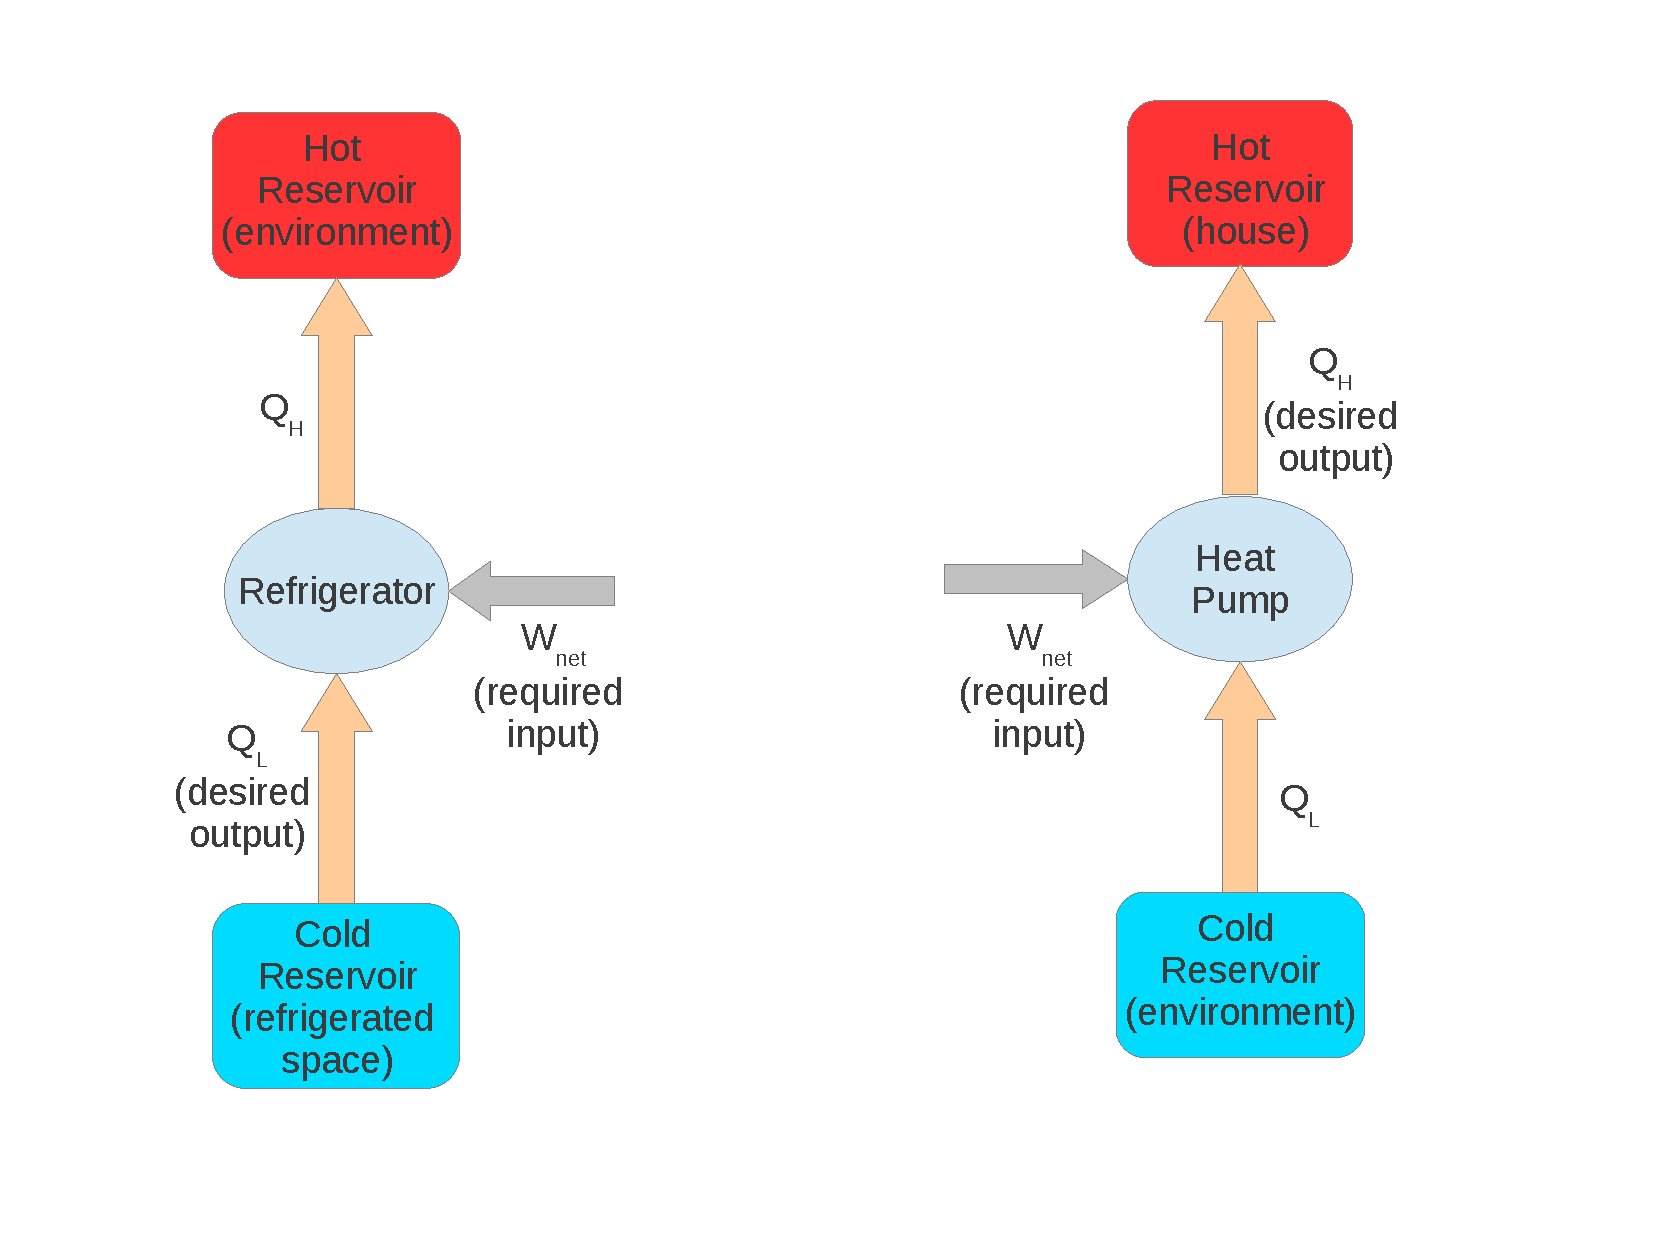
\includegraphics[width=7.5cm,clip]{./Pics/Overview_Refrig2}
     \end{center}
    \end{figure}
   \end{column}  
  \end{columns}
\end{frame}



%%%
%%% Slide
%%%
\begin{frame}
 \frametitle{Refrigerator and Heat Pump}
    \begin{figure}%
     \begin{center}
      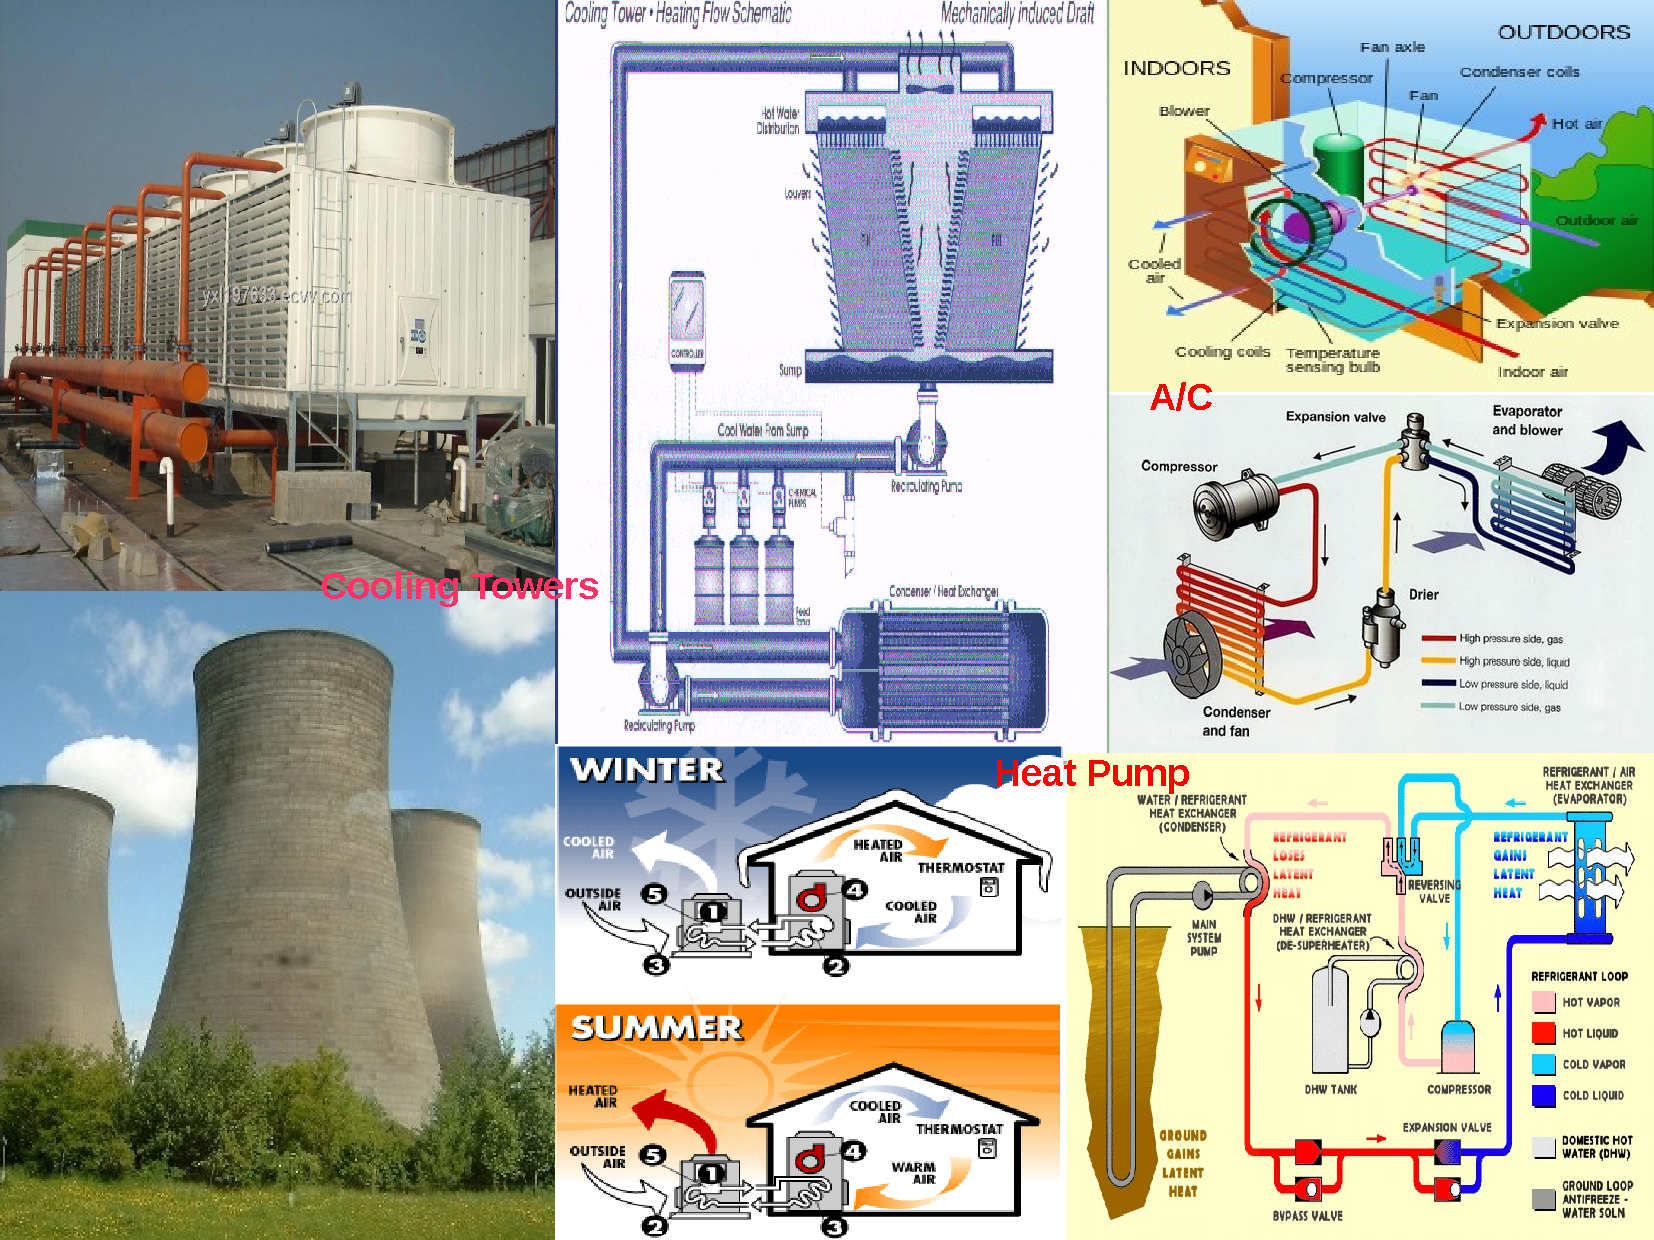
\includegraphics[width=12.cm,height=7.8cm]{./Pics/Overview_Refrig3}
     \end{center}
    \end{figure}
\end{frame}


%%%
%%% Slide
%%%
\begin{frame}
 \frametitle{Coefficient of Performance (COP) and Unit of Refrigeration (Ton)}
    \begin{block}{\begin{center}\scriptsize Coefficient of Performance (COP)\end{center}}\scriptsize
        COP is the ratio of heat absorbed by the refrigerant while passing through the evaporator to the work input required to compress the refrigerant in the compressor, i.e., \blue{ratio between heat extracted and work done,}
        \visible<2->{\begin{equation}
            \text{COP}_{R} =\frc{\text{Desired Output}}{\text{Required Input}}=\frc{\text{Cooling Effect}}{\text{Work Input}}=\frc{Q_{L}}{W_{net,in}} = \frc{Q_{L}}{|Q_{H}|-Q_{L}}\label{Ref1:1}
        \end{equation}}
        \visible<3->{\begin{equation}
            \text{COP}_{HP} = \frc{\text{Desired Output}}{\text{Required Input}}=\frc{\text{Heating Effect}}{\text{Work Input}}=\frc{Q_{H}}{W_{net,in}} = \frc{Q_{H}}{|Q_{H}|-Q_{L}}    \label{Ref1:2}
       \end{equation}}
    \end{block}
     %\item <4-> In other words, it is the ratio between heat extracted and work done;
     %\item <4-> For fixed $Q_{L}$ and $Q_{H}$, Eqns. \ref{Ref1:1} and \ref{Ref1:2} lead to \textcolor{blue}{$\text{COP}_{HP}=\text{COP}_{R}+1$}.
     %\item <4->This means that \textcolor{blue}{COP$_{HP}>1$} (and also \textcolor{red}{COP$_{R}$) is positive}.
     \visible<4->{\begin{block}{\begin{center}\scriptsize Ton of Refrigeration\end{center}}\scriptsize
        \begin{enumerate}[(a)]\scriptsize
           \item<4-> \blue{Refrigeration effect} is the amount of heat extracted by the refrigerator from the refrigerated space;
           \item<4-> This effect is quantified by the \blue{unit of refrigeration} or \red{Ton of refrigeration};
           \item<4-> \red{One Ton (or Tonne)} of refrigeration is defined as the amount of heat removed from 1000 kg of water at 0$^{\text{o}}$C to form 1000 kg of ice within 24 hours. This quantifies the latent heat $\left(L_{f}\right)$ required to be removed for solidification of water at 0$^{\text{o}}$C, i.e.,
      \end{enumerate}
         \visible<5->{\begin{displaymath}
              \textcolor{red}{\text{1 Ton of Refrigeration}} = \text{mass of water} \times L_{f} = \text{ 12000 BTU/h} \sim \textcolor{blue}{210\;\; \text{kJ/min}} = \text{ 3.5 kW}\nonumber 
         \end{displaymath}}
     \end{block}}
 % \end{enumerate}
\end{frame}

%%%
%%% SECTION
%%%
\subsection{Vapour-Compression Refrigeration Cycle}


%%%
%%% Slide
%%%
\begin{frame}
 \frametitle{Introduction}

  \scriptsize A few animations for reversed Brayton, Rankine cycles can be found in:
\href{http://www.sfsb.unios.hr/test/testhome/vtAnimations/animations/chapter09/refrigeration/index1.html}{\scriptsize{http://www.sfsb.unios.hr/test/testhome/vtAnimations/animations/chapter09/refrigeration/index1.html}}


  \begin{columns}
   \begin{column}[c]{0.45\linewidth}
    \begin{figure}%
     \begin{center}
      \visible<2->{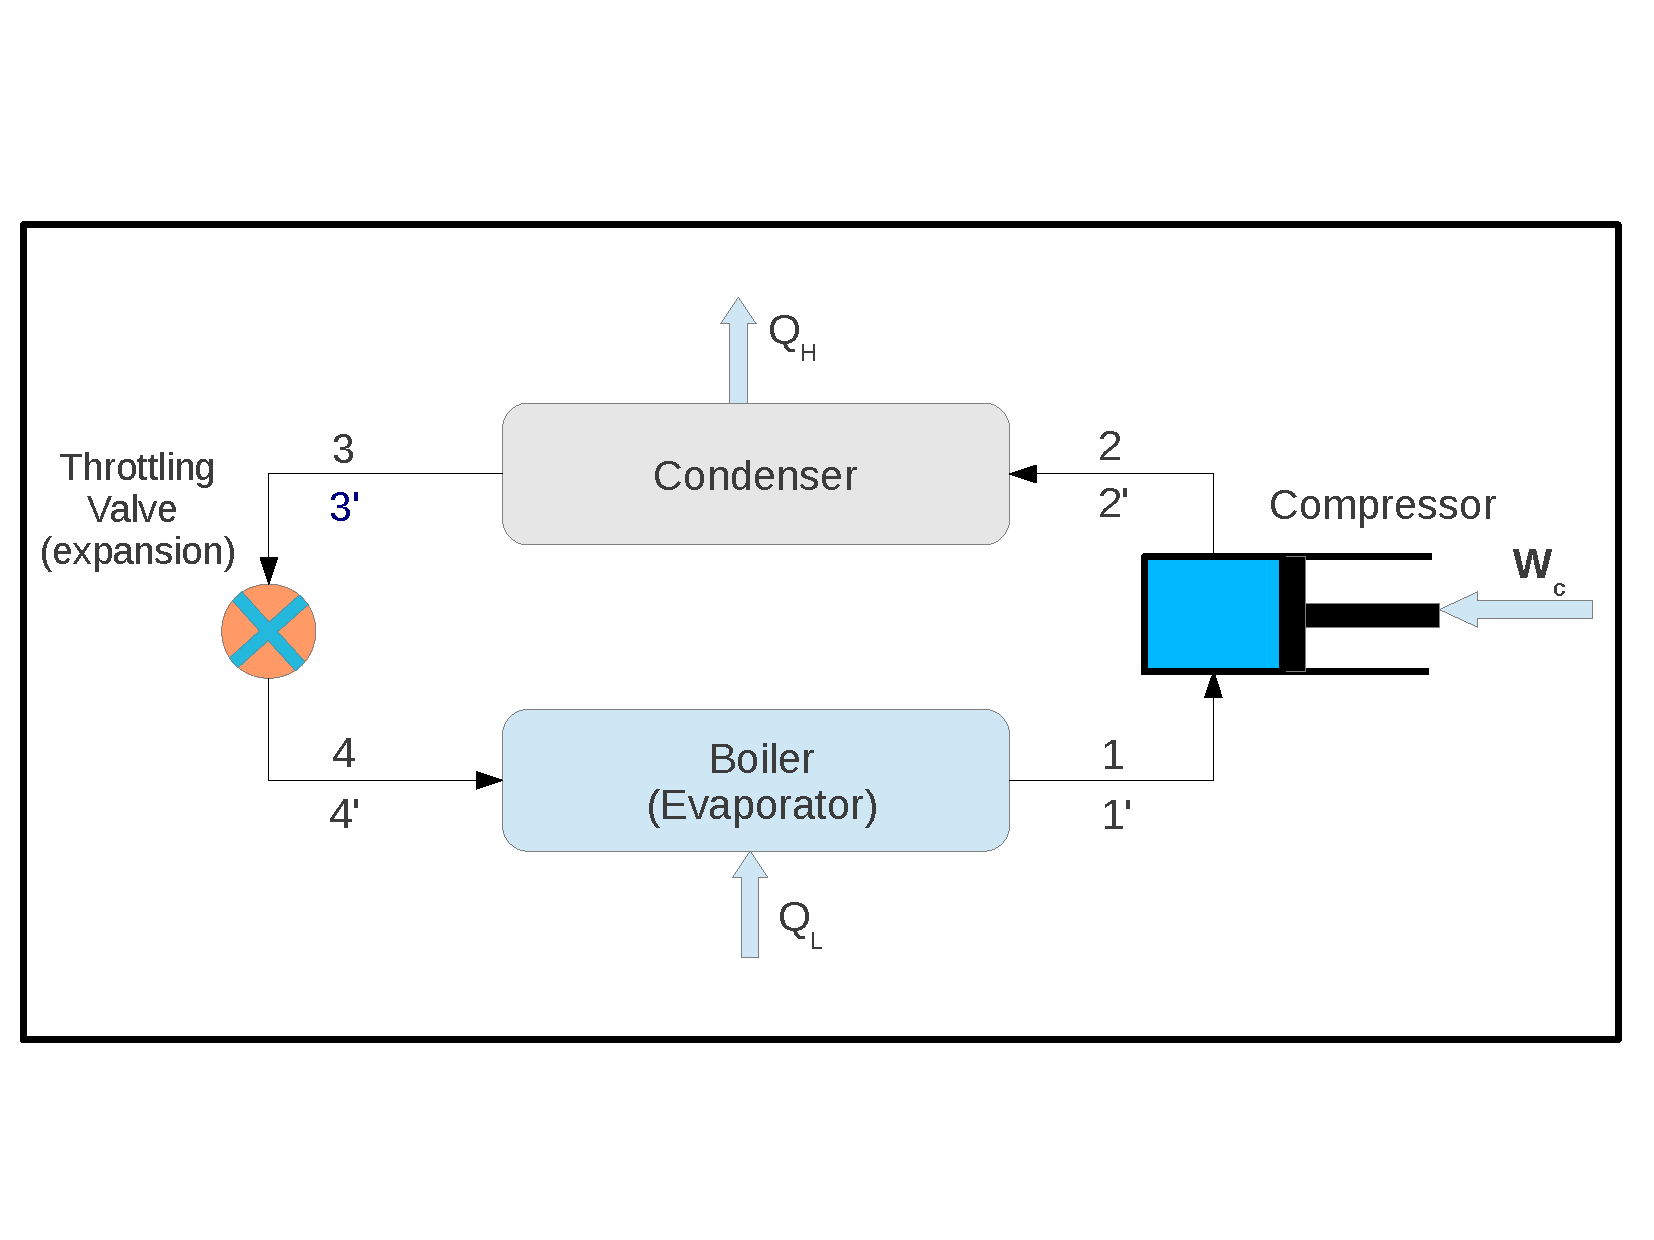
\includegraphics[width=\columnwidth,clip]{./Pics/Overview_Refrig12}}
     \end{center}
    \end{figure}  
   \end{column}  
   \begin{column}[c]{0.55\linewidth}
  \begin{enumerate}[(1)]\scriptsize
   \item <2-> First vapour-compression refrigeration system was a closed system introduced by Jacob Perkins (1766-1849) using \textcolor{blue}{diethyl ether} as refrigerant fluid;
   \item <2-> Ether vapour was compressed in a piston-cylinder system and condensed (i.e., turned into liquid) at a higher saturation pressure and temperature;
   \item <2-> Liquid ether is throttled through a valve back into the low-pressure evaporator;
   \item <2-> This process takes place beneath the vapour dome of the ether and it is a \textcolor{blue}{reversed Rankine cycle}.
   \item <3-> In most industrial applications, vapour compression systems occur in closed cycles.
  \end{enumerate}
 \end{column}  
\end{columns}

\end{frame}


%%%
%%% Slide
%%%
\begin{frame}
 \frametitle{Dry Compression Cycle} 
  \begin{columns}
   \begin{column}[c]{0.5\linewidth}
    \begin{figure}%
     \vbox{
      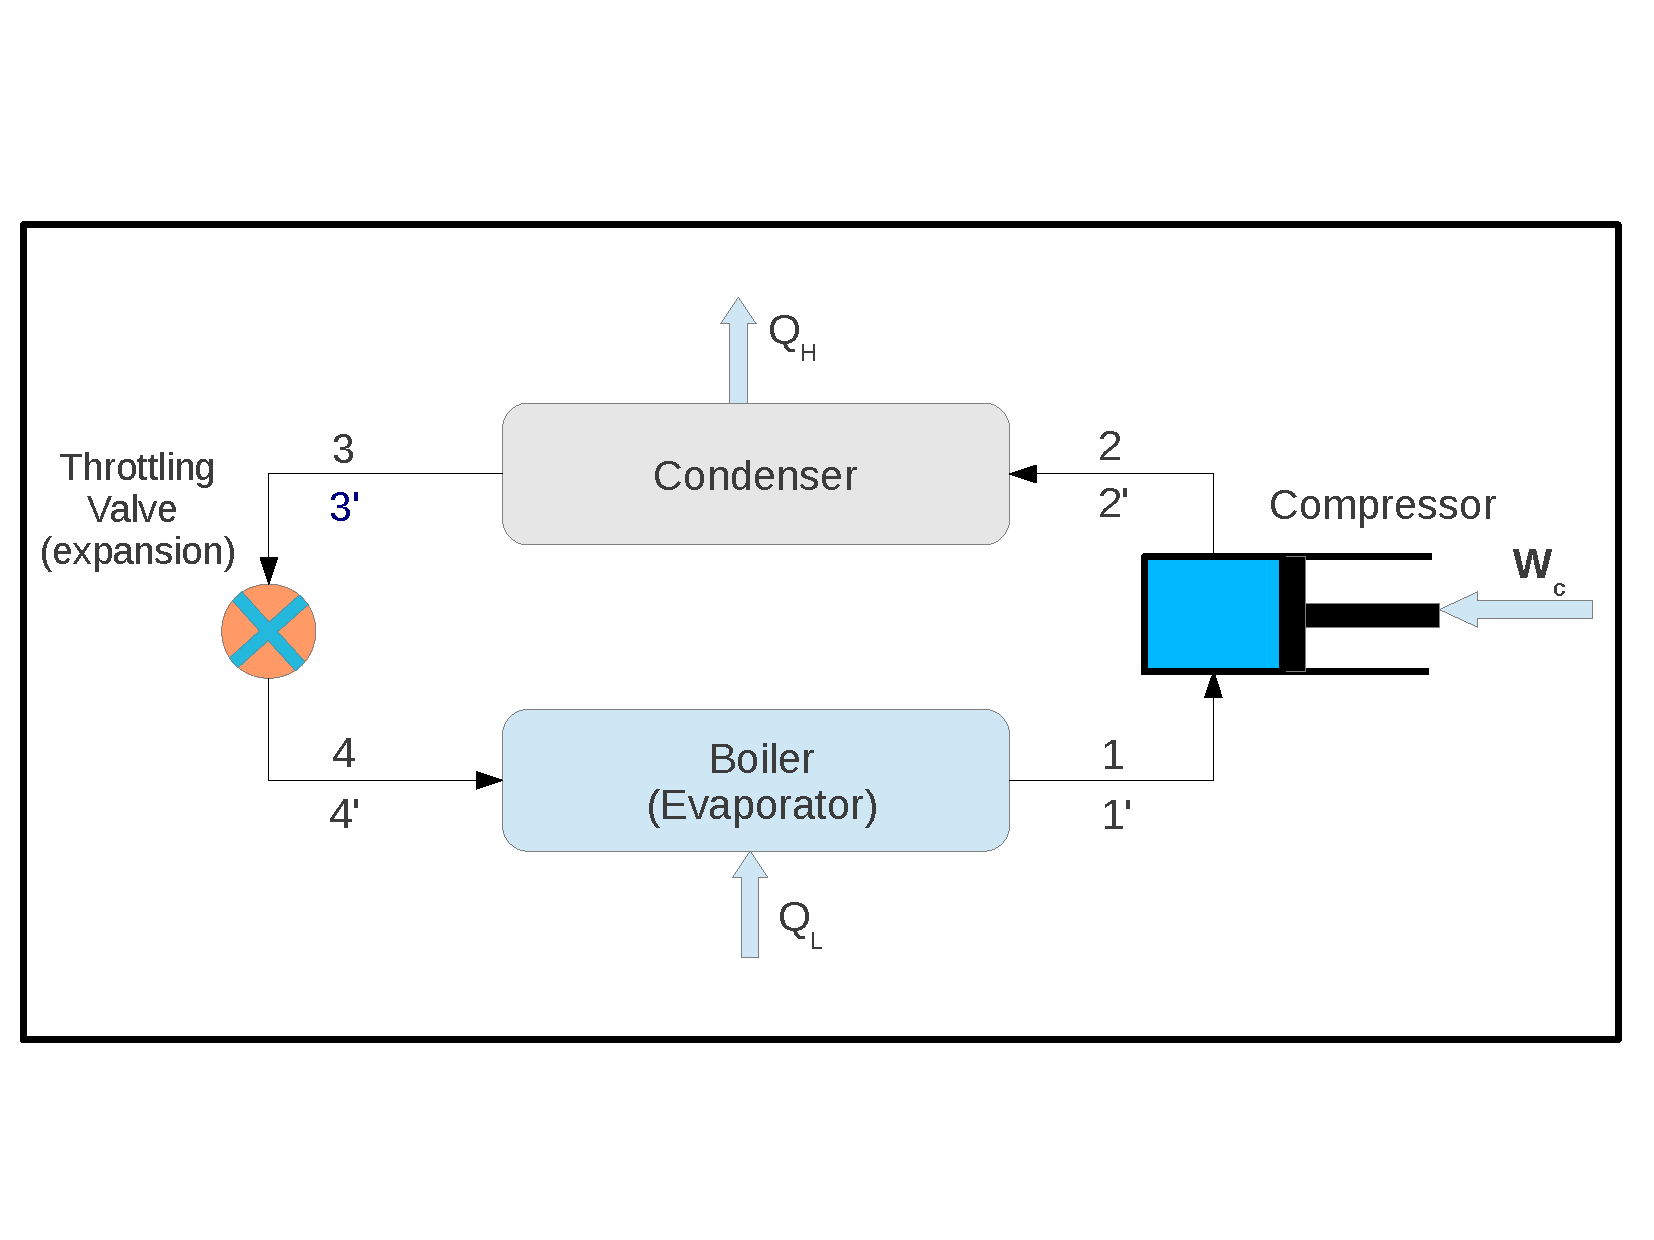
\includegraphics[width=5.5cm,clip]{./Pics/Overview_Refrig12}
      \vspace{-.5cm}
      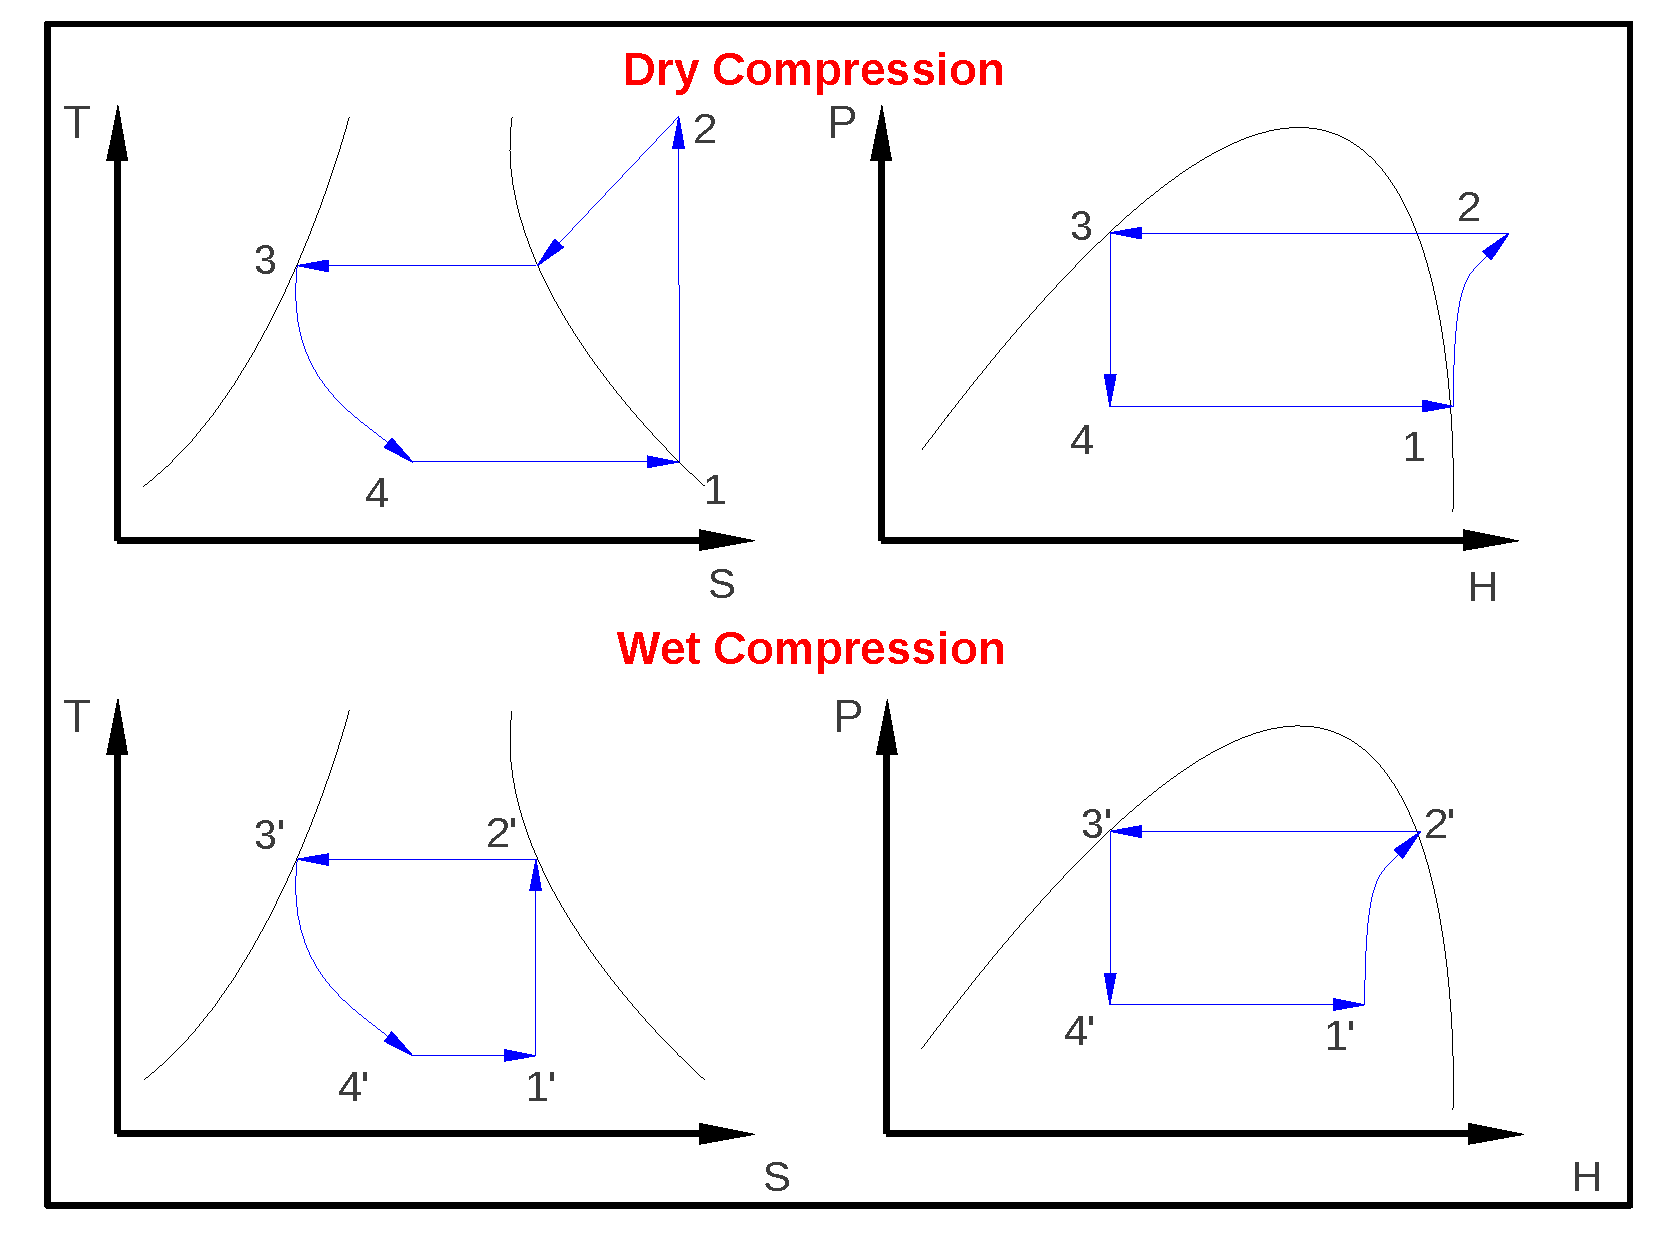
\includegraphics[width=4.5cm,clip]{./Pics/Overview_Refrig13}}
    \end{figure}  
   \end{column}  
   \begin{column}[c]{0.5\linewidth}
  \begin{enumerate}[(1)] \scriptsize
   \item <1-> Refrigerant (in gas/vapour phase) is compressed isentropically in \textcolor{blue}{compressor from state 1 to 2}; 
   \item <1-> \textcolor{blue}{High pressure and high temperature} fluid enters the condenser at \textcolor{blue}{state 2};
   \item <1-> The condensed fluid (saturated liquid at high pressure, state 3) is driven into the expansion valve where an \textcolor{blue}{isenthalpic expansion} occurs.
   \item <1-> The refrigerant fluid leaves the expansion valve (state 4) as a \textcolor{blue}{low pressure wet mixture of liquid and vapour};
   \item <2-> This mixture is driven into the evaporator where heat is transferred from the surroundings and thereby showing refrigerant effect; 
   \item <2-> Due to this \textcolor{blue}{heat absorption}, the liquid-vapour mixture is transformed into a \textcolor{red}{dry gaseous refrigerant} and;
   \item <3-> This process is called \textcolor{blue}{\underline{Dry Compression}} in which,
   \item <3-> The compression of this dry refrigerant yields \textcolor{blue}{superheated state} of the fluid as shown in \textcolor{blue}{state 2}.
  \end{enumerate}
 \end{column}  
\end{columns}
\end{frame}


%%%
%%% Slide
%%%
\begin{frame}
 \frametitle{Wet Compression Cycle} 
  \begin{columns}
   \begin{column}[c]{0.5\linewidth}
    \begin{figure}%
     \vbox{
      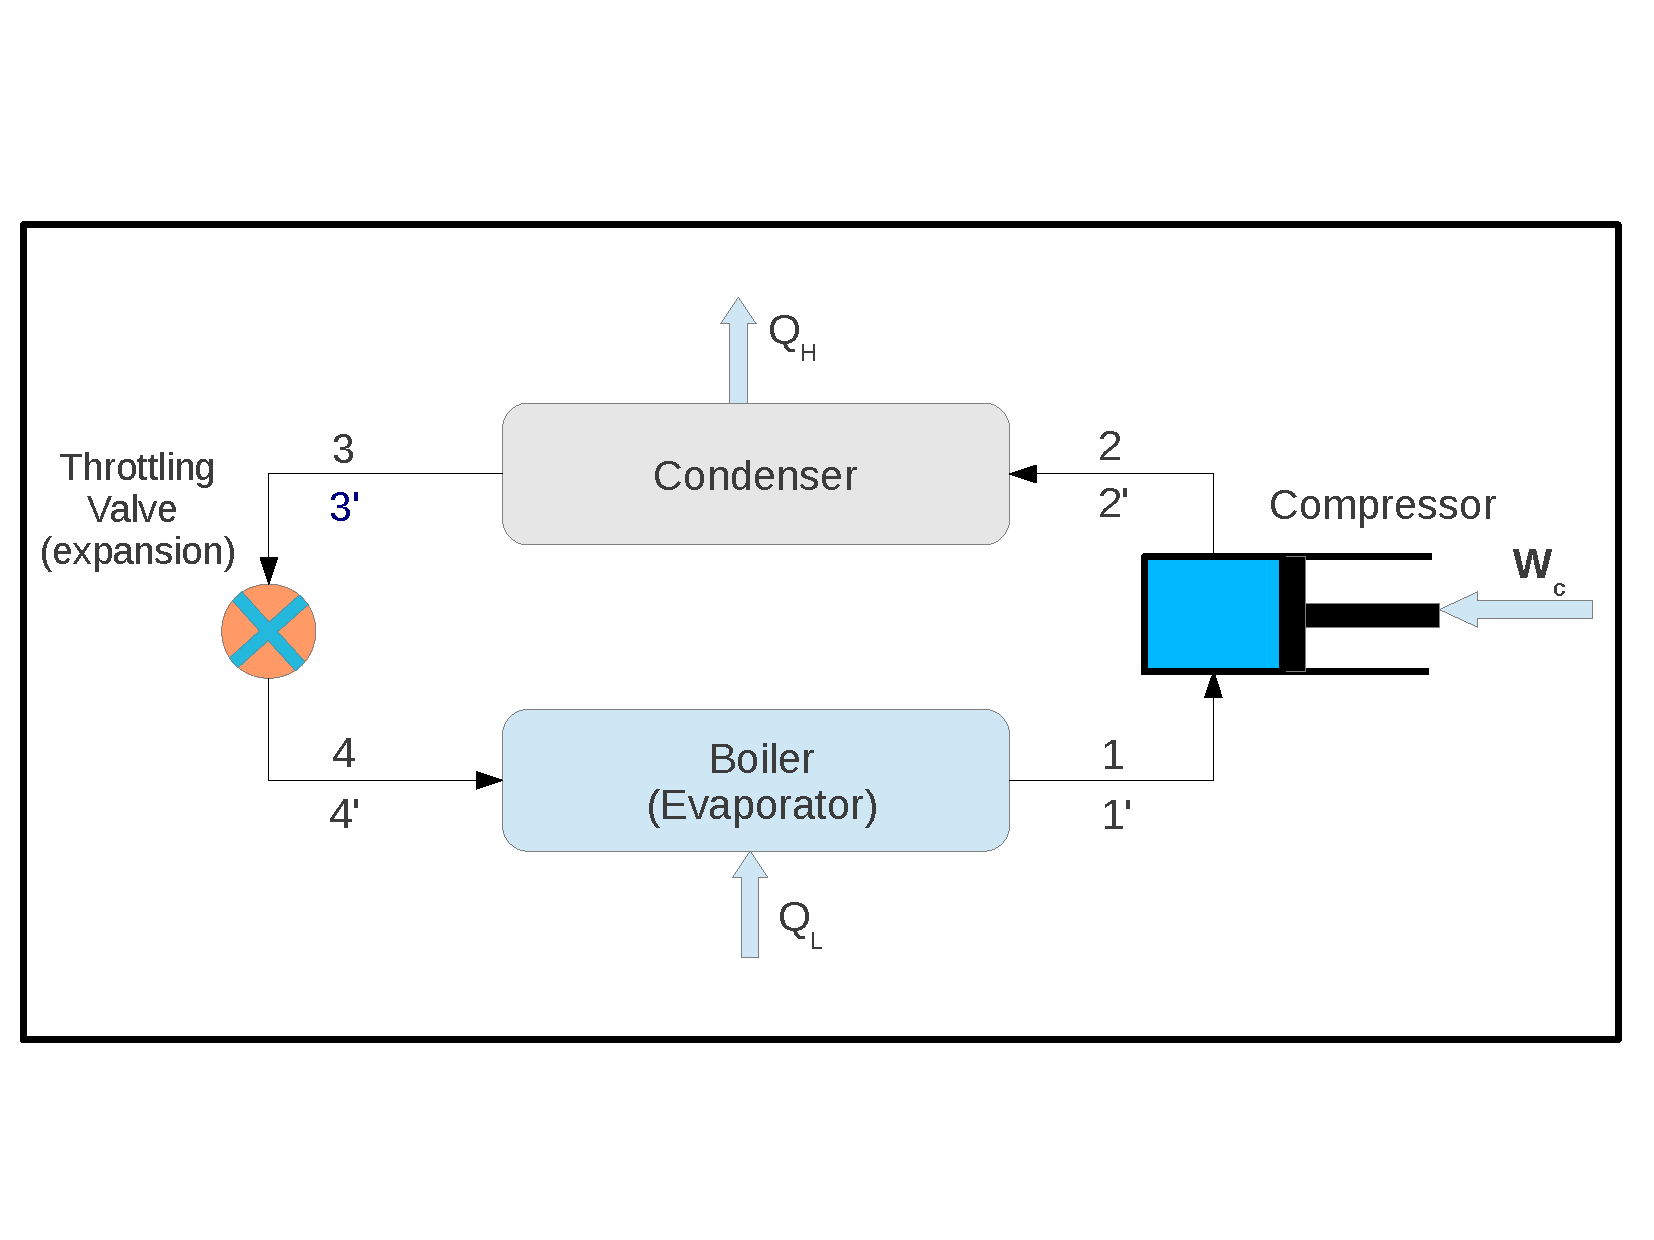
\includegraphics[width=5.5cm,clip]{./Pics/Overview_Refrig12}
      \vspace{-.5cm}
      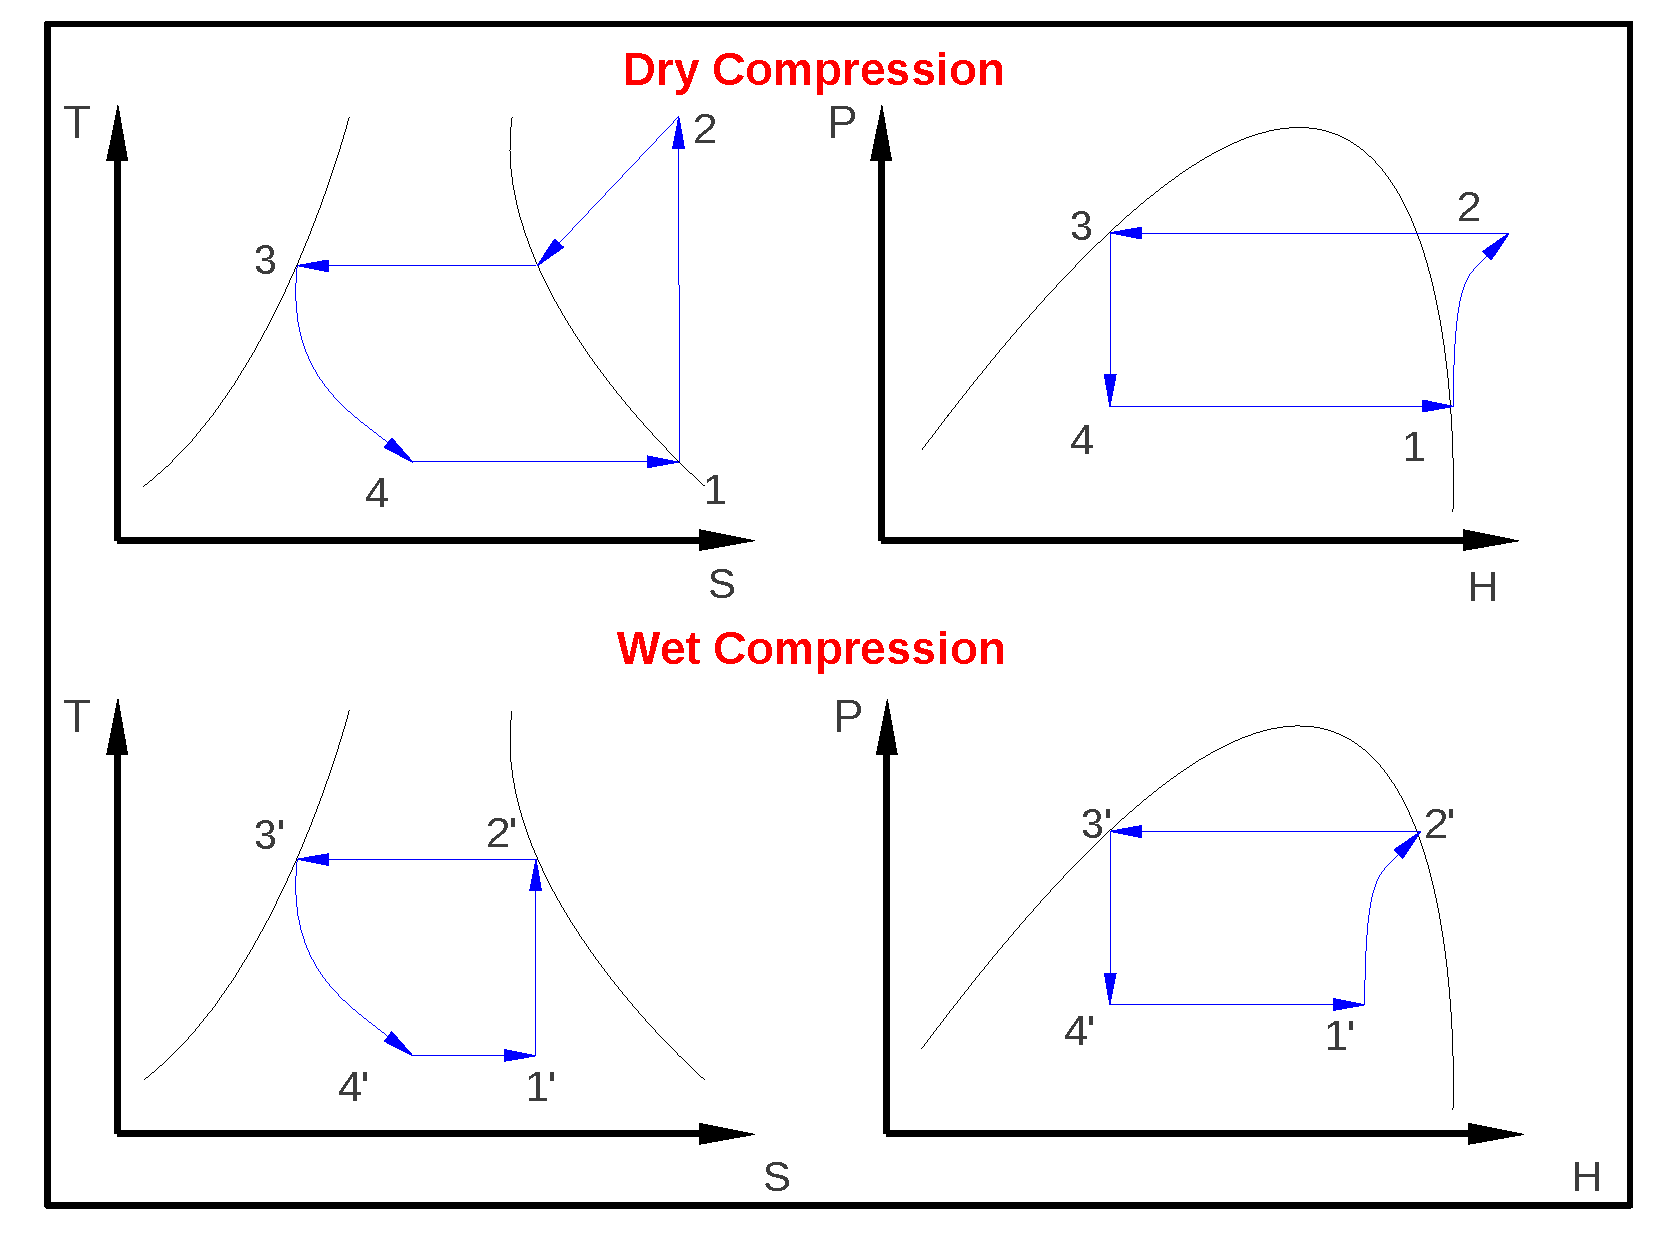
\includegraphics[width=4.5cm,clip]{./Pics/Overview_Refrig13}}
    \end{figure}  
   \end{column}  
   \begin{column}[c]{0.5\linewidth}
  \begin{enumerate}[(1)] \setcounter{enumi}{8}\scriptsize
     \item <1-> In this case, the \textcolor{blue}{liquid-vapour mixture (state 1$^{\prime}$)} is injected in the compressor;
     \item <1-> In the compressor, the wet mixture is transformed into a \textcolor{blue}{dry refrigerant fluid} (gas phase -- state 2$^{\prime}$);
     \item <1-> The dry refrigerant at \textcolor{blue}{high pressure and high temperature} is driven into the condenser where the fluid is turned into saturated liquid at high pressure;
     \item <1-> The refrigerant is throttled from high to low pressure inside the expansion valve (states 3$^{\prime}$-4$^{\prime}$);
     \item <1-> The refrigerant is then driven towards the evaporator (states 4$^{\prime}$ 1$^{\prime}$) where it absorbs heat from the surroundings and ;
     \item <1-> Part of the liquid fraction is evaporated \textcolor{red}{but it does not become dry (gas) refrigerant} at the inlet of the compressor.

  \end{enumerate}
 \end{column}  
\end{columns}
\end{frame}



%%%
%%% Slide
%%%
\begin{frame}
 \frametitle{Thermodynamic Analysis} 
  \begin{columns}
   \begin{column}[c]{0.6\linewidth}
     \begin{enumerate}[(1)]\scriptsize
       \item<1-> Four Stages:
         \begin{enumerate}[(a)]\scriptsize
            \item <1-> 1-2 or 1$^{\prime}$-2$^{\prime}$: isentropic compression;
            \item <1-> 2-3 or 2$^{\prime}$-3$^{\prime}$: isobaric heat rejection;
            \item <1-> 3-4 or 3$^{\prime}$-4$^{\prime}$: isenthalpic expansion ;%process or throttling process;
            \item <1-> 4-1 or 4$^{\prime}$-1$^{\prime}$: isobaric heat absorption.
         \end{enumerate}
       \item<2-> For a mass flow rate of refrigerant \blue{$\dot{m}$} (kg/s):
         \begin{enumerate}[(a)]\scriptsize
           \item<2-> The \blue{refrigeration capacity} (or refrigeration effect) is,\\
               \visible<2->{\begin{displaymath}
                Q_{\text{absorbed}}^{\text{(dry)}} = \dot{m}\left(h_{1}-h_{4}\right) \;\text{;}\; Q_{\text{absorbed}}^{\text{(wet)}} = \dot{m}\left(h_{1^{\prime}}-h_{4^{\prime}}\right)         
             \end{displaymath}}
           \item <3-> And the \blue{net work} (= work input) is,
             \visible<3->{\begin{displaymath}     
                W_{\text{compressor}}^{\text{(dry)}} = \dot{m}\left(h_{2}-h_{1}\right) \;\text{;}\; W_{\text{compressor}}^{\text{(wet)}} = \dot{m}\left(h_{2^{\prime}}-h_{1^{\prime}}\right) 
             \end{displaymath}}
           \item<4-> And the \blue{Coefficient of Performance (COP)} is,
             \visible<4->{\begin{eqnarray}
                && COP^{\text{(dry)}} = \frc{\text{Refrigeranting Capacity}}{\text{Work done}} = \frc{h_{1}-h_{4}}{h_{2}-h_{1}}   \nonumber \\ 
                && COP^{\text{(wet)}} = \frc{h_{1^{\prime}}-h_{4^{\prime}}}{h_{2^{\prime}}-h_{1^{\prime}}} \nonumber
             \end{eqnarray}}
         \end{enumerate}
     \end{enumerate}
   \end{column}  
   \begin{column}[c]{0.4\linewidth}
     \vbox{
      \hbox{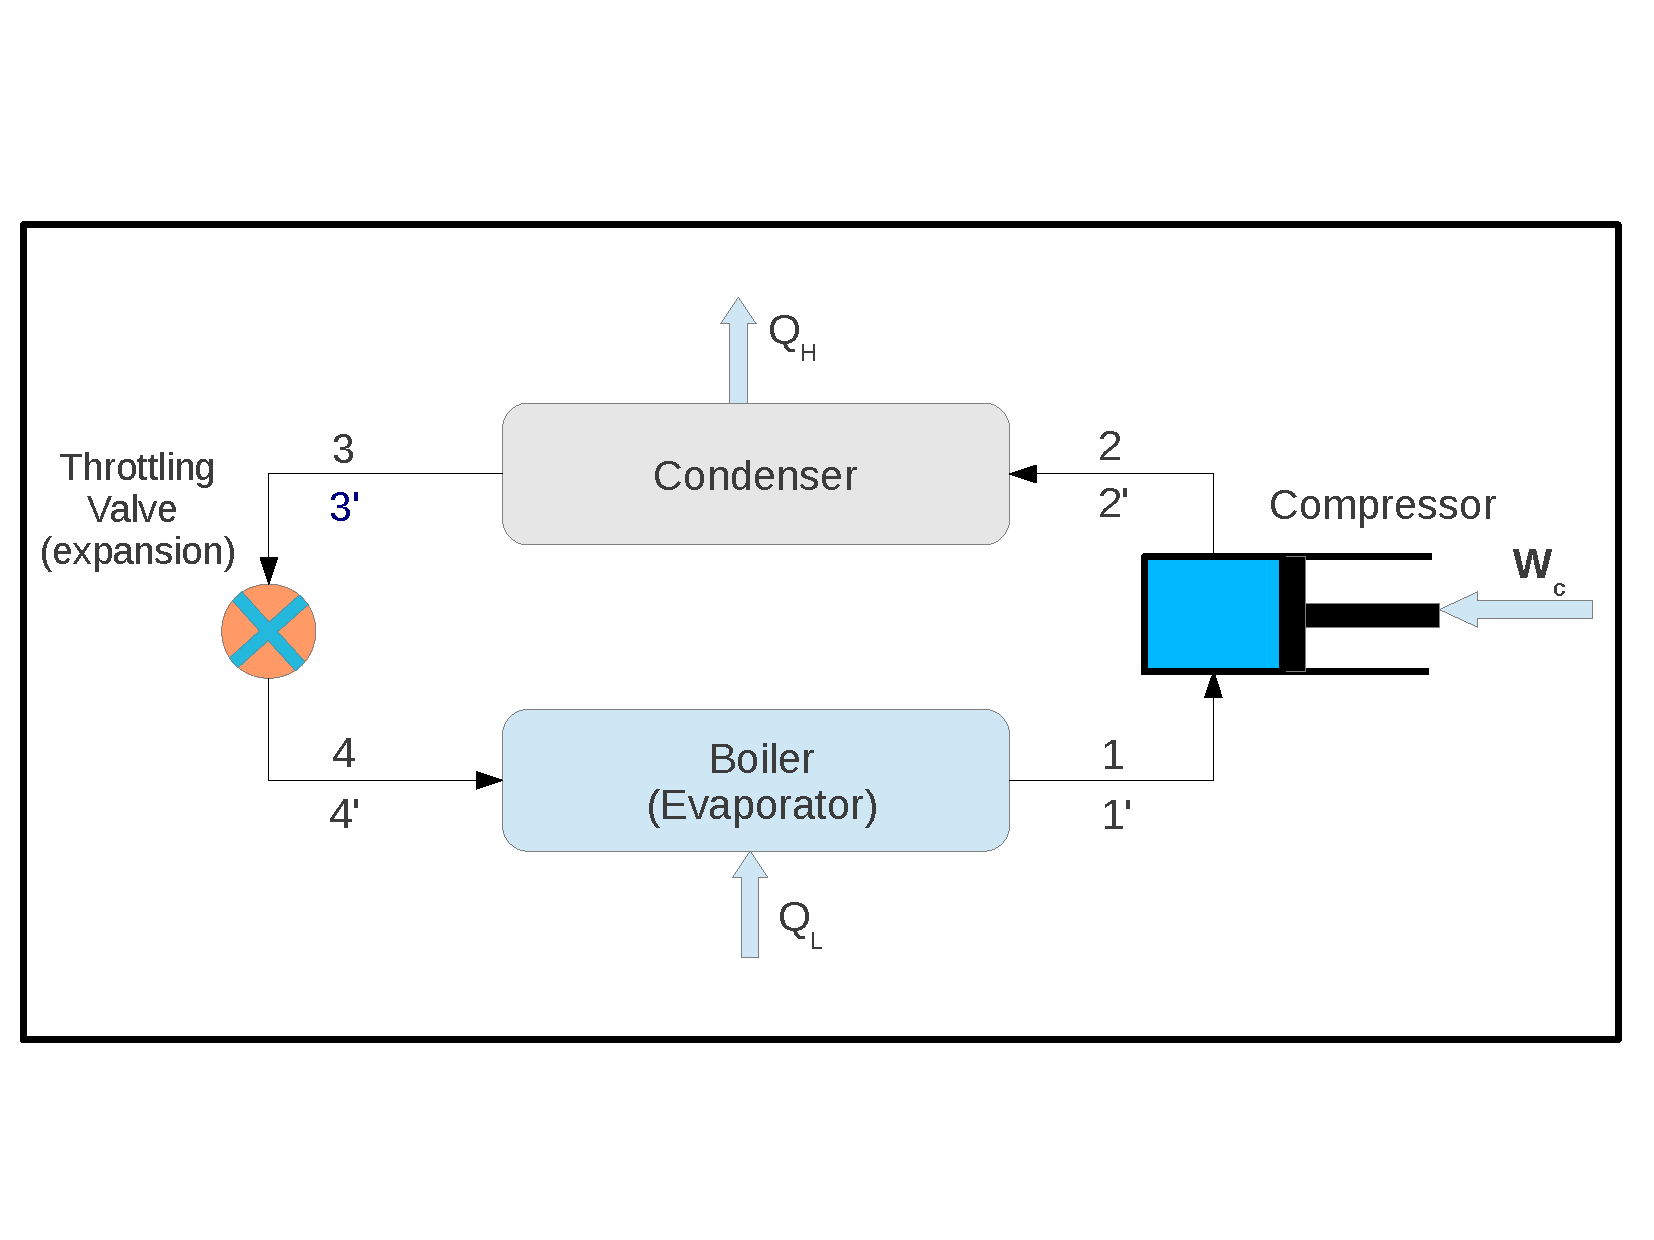
\includegraphics[width=.9\columnwidth]{./Pics/Overview_Refrig12}}
      \hbox{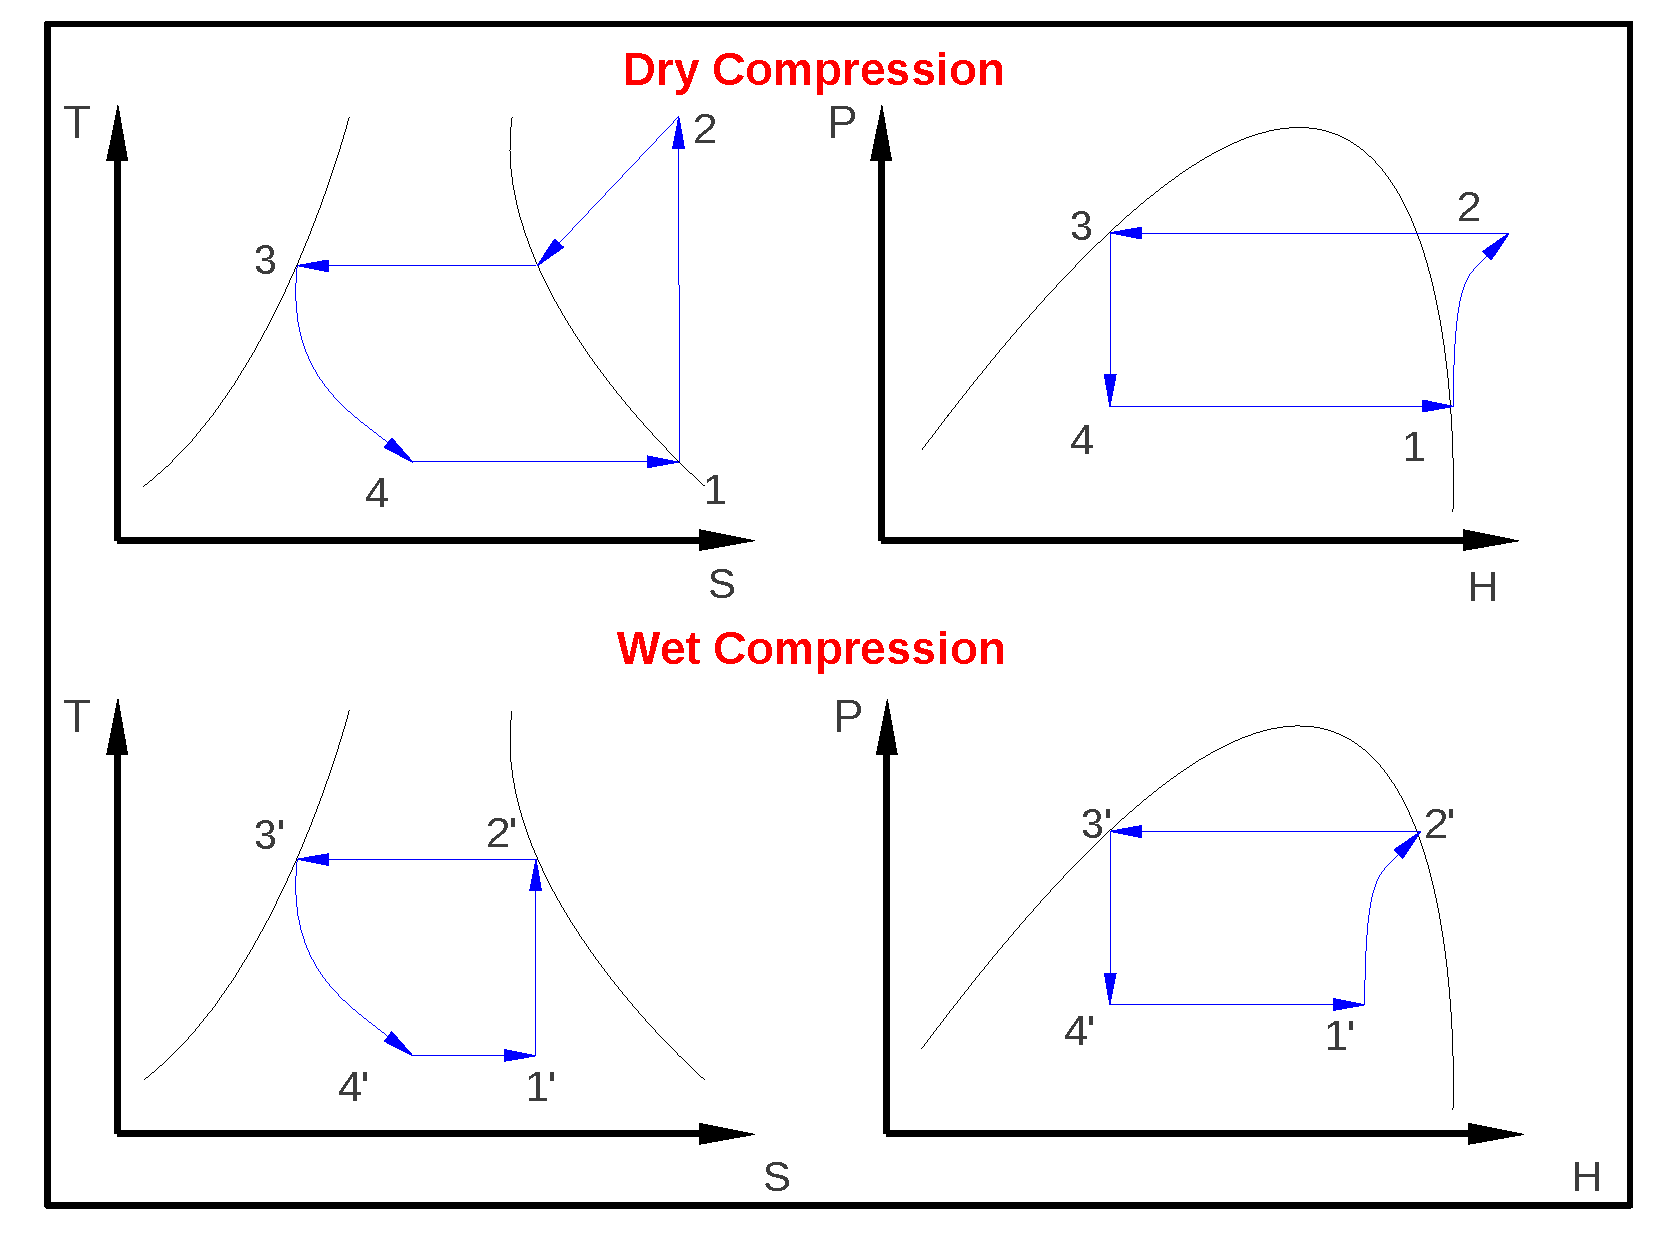
\includegraphics[width=.9\columnwidth]{./Pics/Overview_Refrig13}}}
   \end{column}  

\end{columns}
\end{frame}
 

%%%
%%% Slide
%%%
\begin{frame}
 \frametitle{Thermodynamic Analysis} 
   \begin{figure}%
     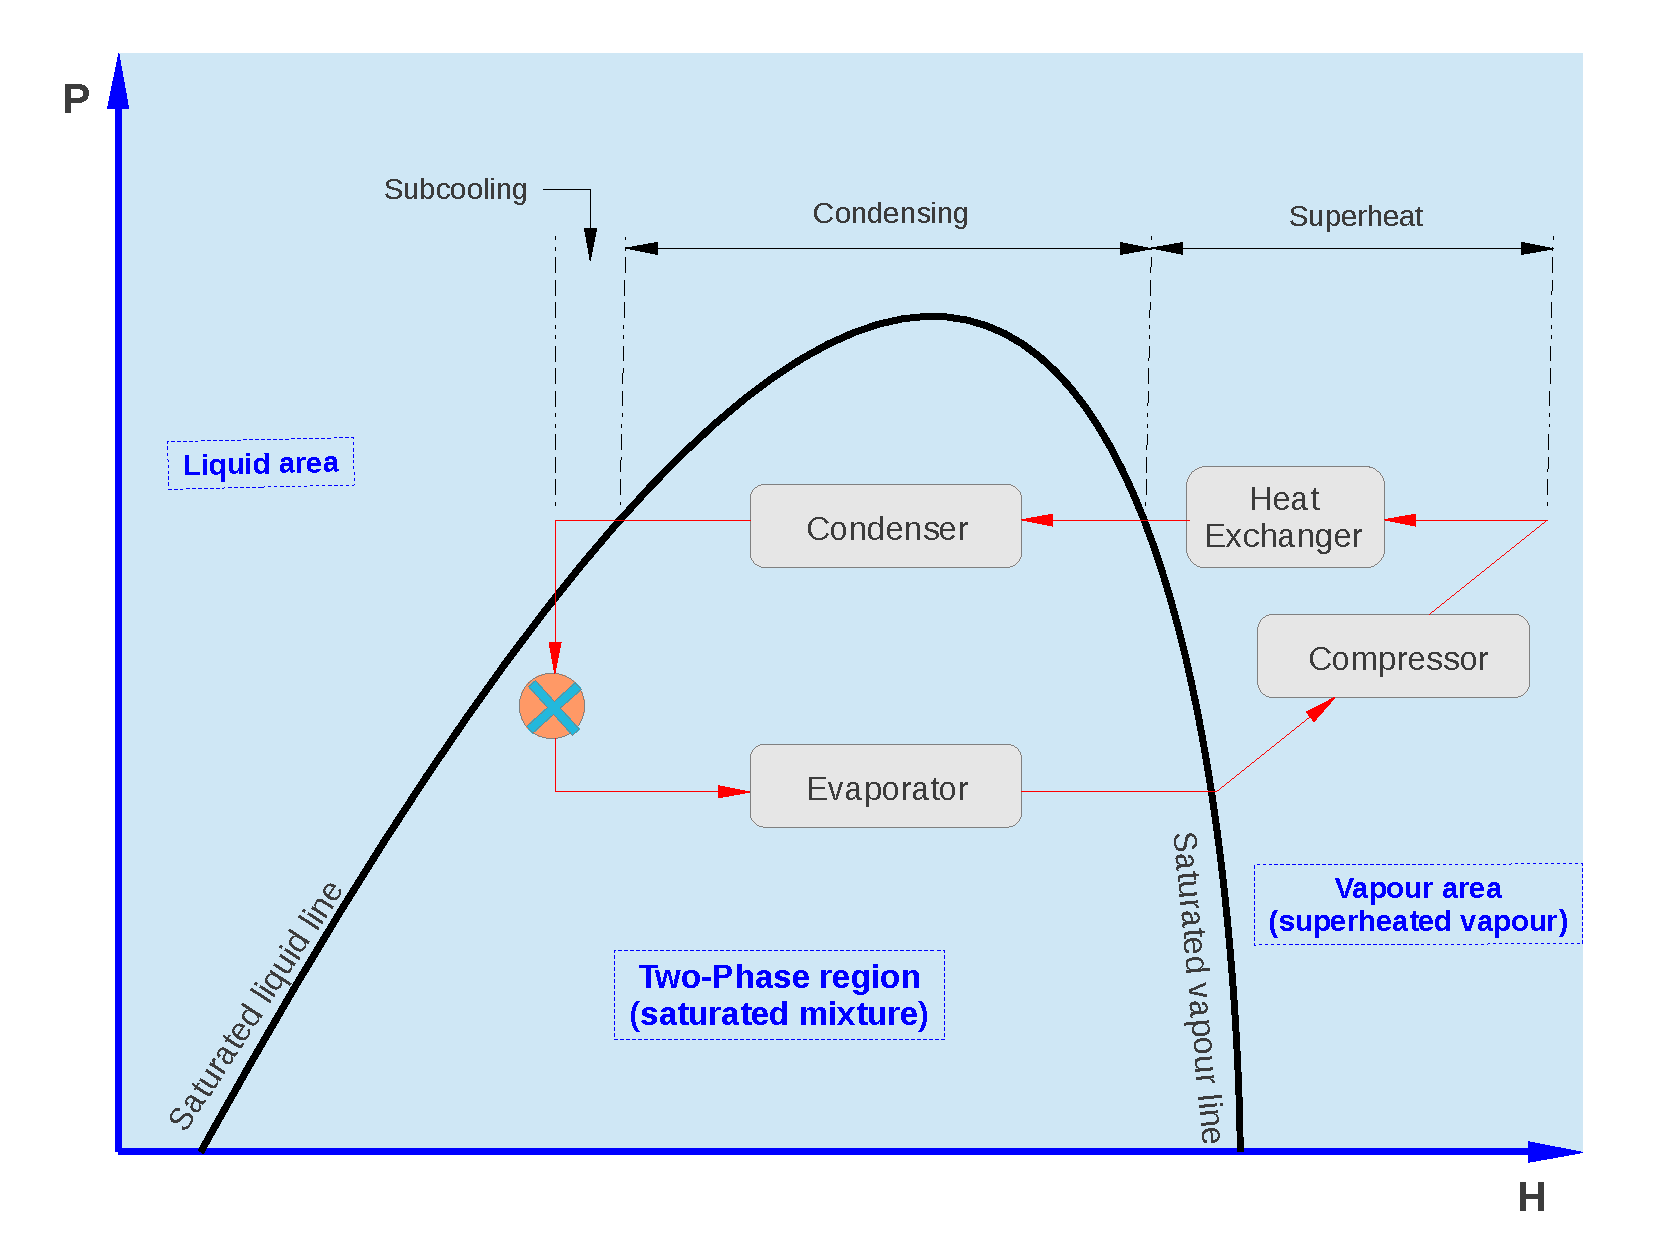
\includegraphics[width=.8\columnwidth]{./Pics/Overview_Refrig19}
   \end{figure}
\end{frame}

%%%
%%% SECTION
%%%
\subsection{Heat Pumps}

%%%
%%% Slide
%%%
\begin{frame}
 \frametitle{Heat Pumps}
    \begin{figure}%
     \begin{center}
      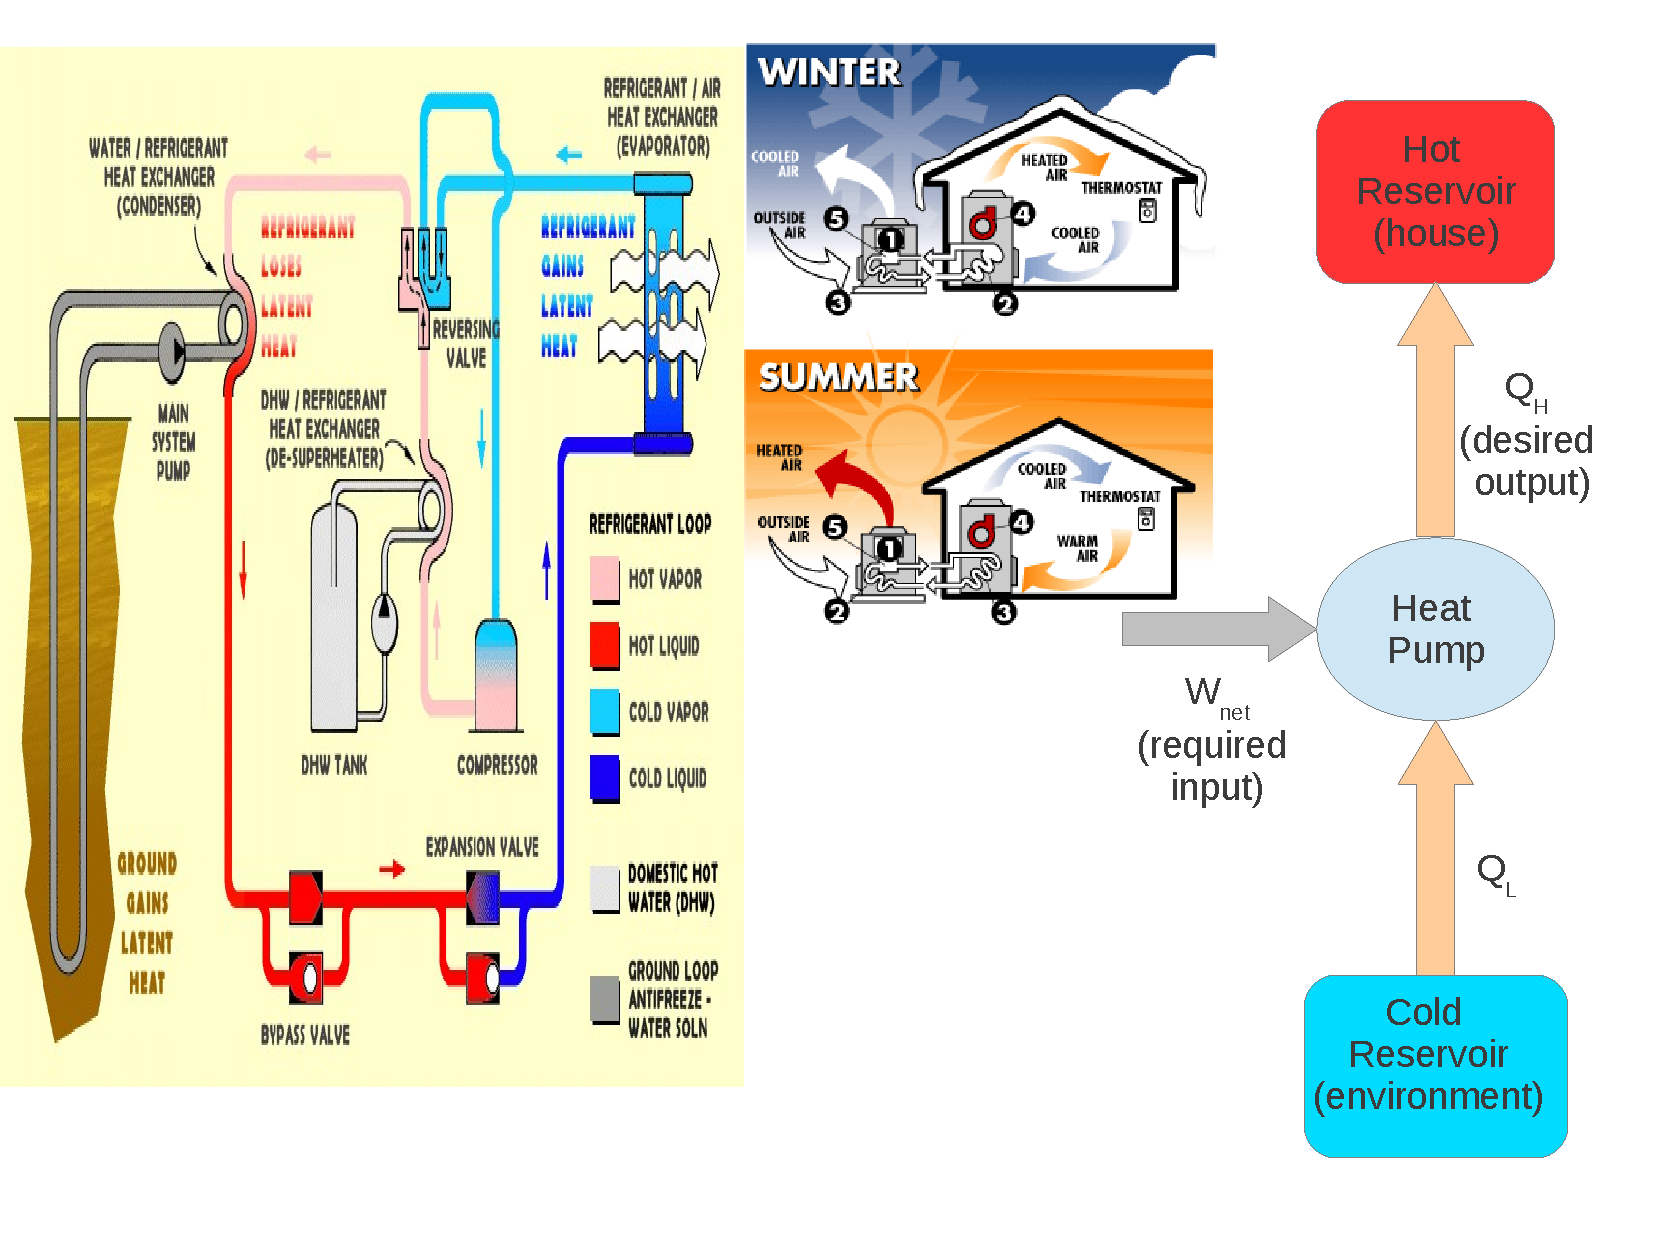
\includegraphics[width=12.cm,height=7.8cm]{./Pics/Overview_Refrig35}
     \end{center}
    \end{figure}
\end{frame}



%%% Slide
%%%
\begin{frame}
 \frametitle{Objectives}
  \begin{columns}
   \begin{column}[c]{0.45\linewidth}
  \begin{enumerate}[(i)]\scriptsize
   \item <1-> \textcolor{blue}{Heat Pumps} are devices that are used to \textcolor{blue}{maintain} a body at a temperature larger than the surroundings;
   \item <2-> They work in a very similar way as the refrigerators we have studied, but with \textcolor{red}{a difference} in the objective;
   \item <3-> \textcolor{blue}{HPs} keep the temperature of the body above to the temperature in the surroundings whereas;
   \item <4-> The \textcolor{blue}{refrigerators} maintain the temperature below the surrounding temperature.
   \item <5-> \textcolor{blue}{HPs} can be based on vapour-compression cycle, absorption cycle, etc;
   \item <6-> The figure in the rhs is a vapour-compression cycle representation of the heat pump, where \textcolor{blue}{heat} is removed in the \textcolor{blue}{condenser};
   \item <7-> The \textcolor{blue}{Coefficient of Performance} for HP (1.5 $\lq$ COP $\lq$ 4) is given by
    \begin{eqnarray}
     \textcolor{blue}{\text{COP}} &=& \frc{\text{Desired Effect (heating of space)}}{\text{Net Work}} \nonumber \\
                                  &=& \textcolor{blue}{\frc{h_{3}-h_{2}}{h_{2}-h_{1}}}
    \end{eqnarray}
  \end{enumerate}
   \end{column}
   \begin{column}[c]{0.55\linewidth}
    \begin{figure}%
     \begin{center}
      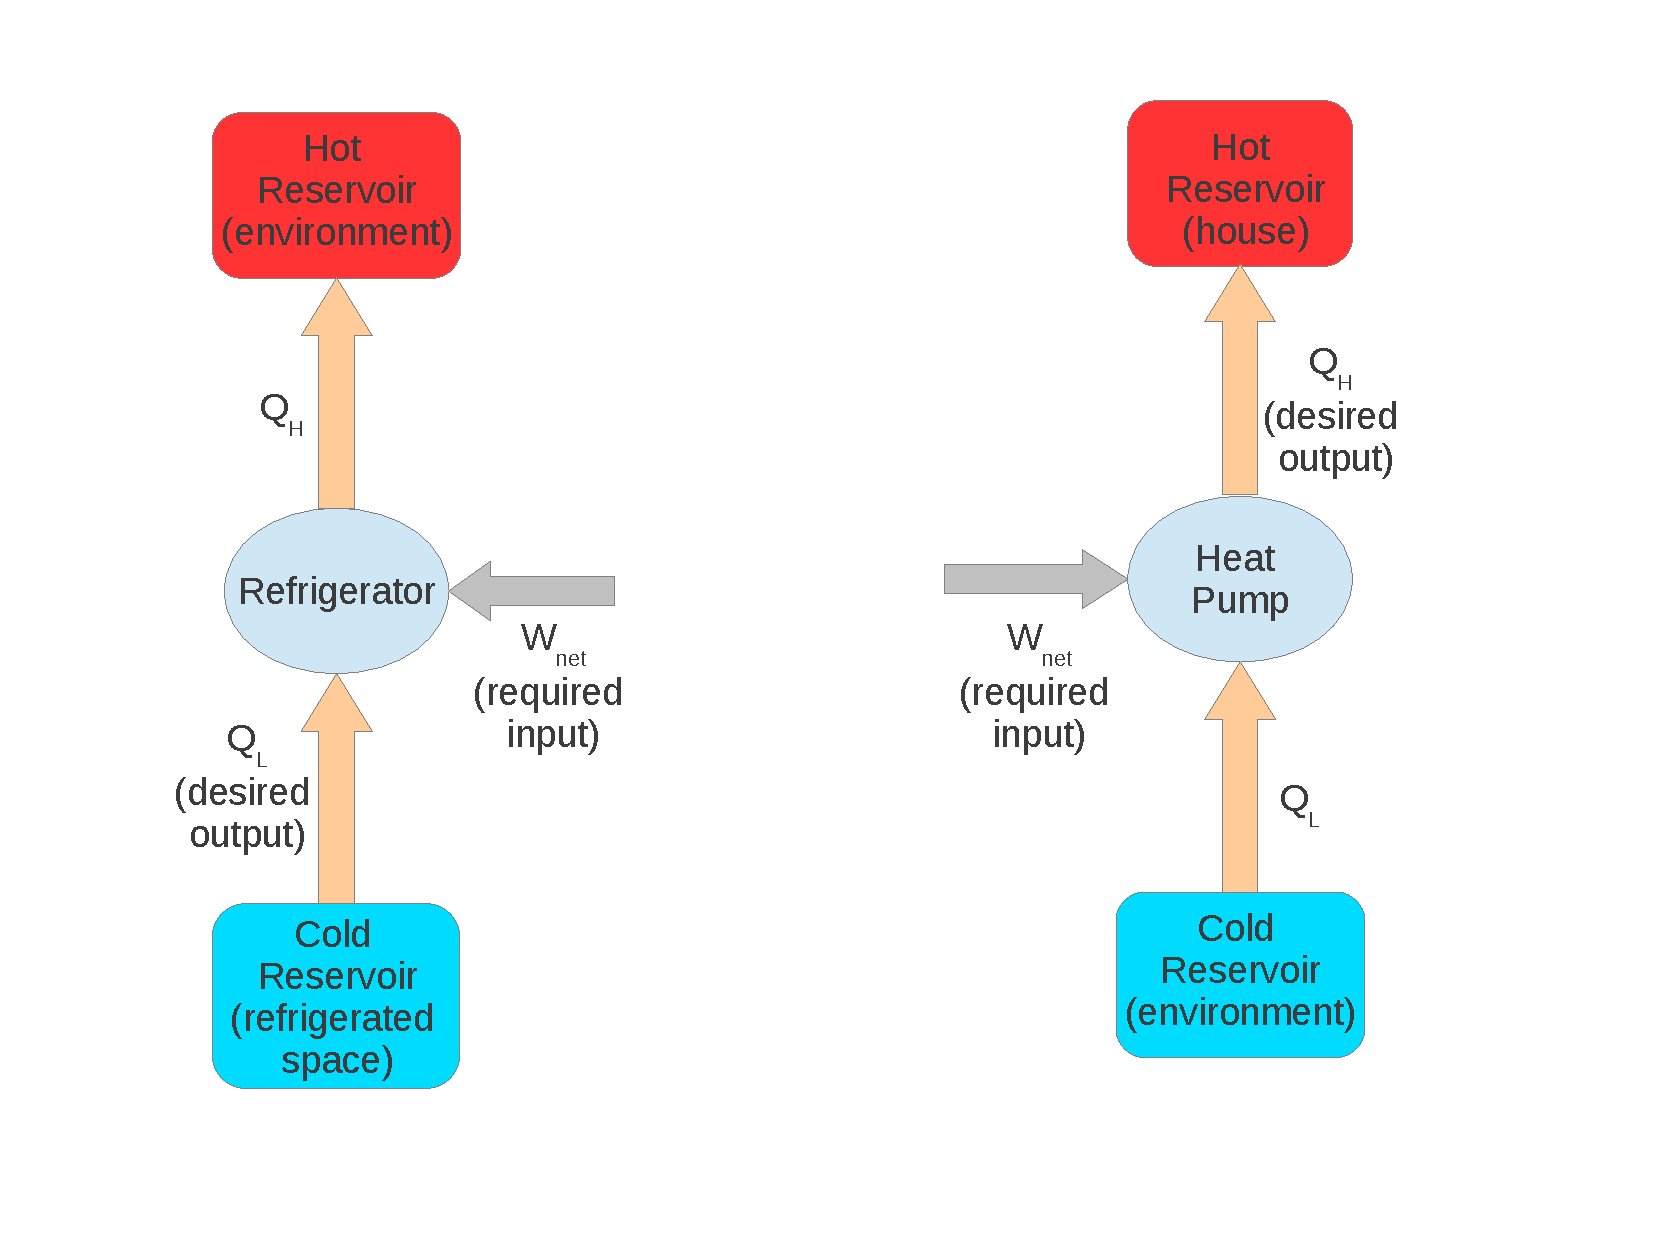
\includegraphics[width=6.5cm,clip]{./Pics/Overview_Refrig2} \\
       \vspace{-.5cm}
      \visible<6->{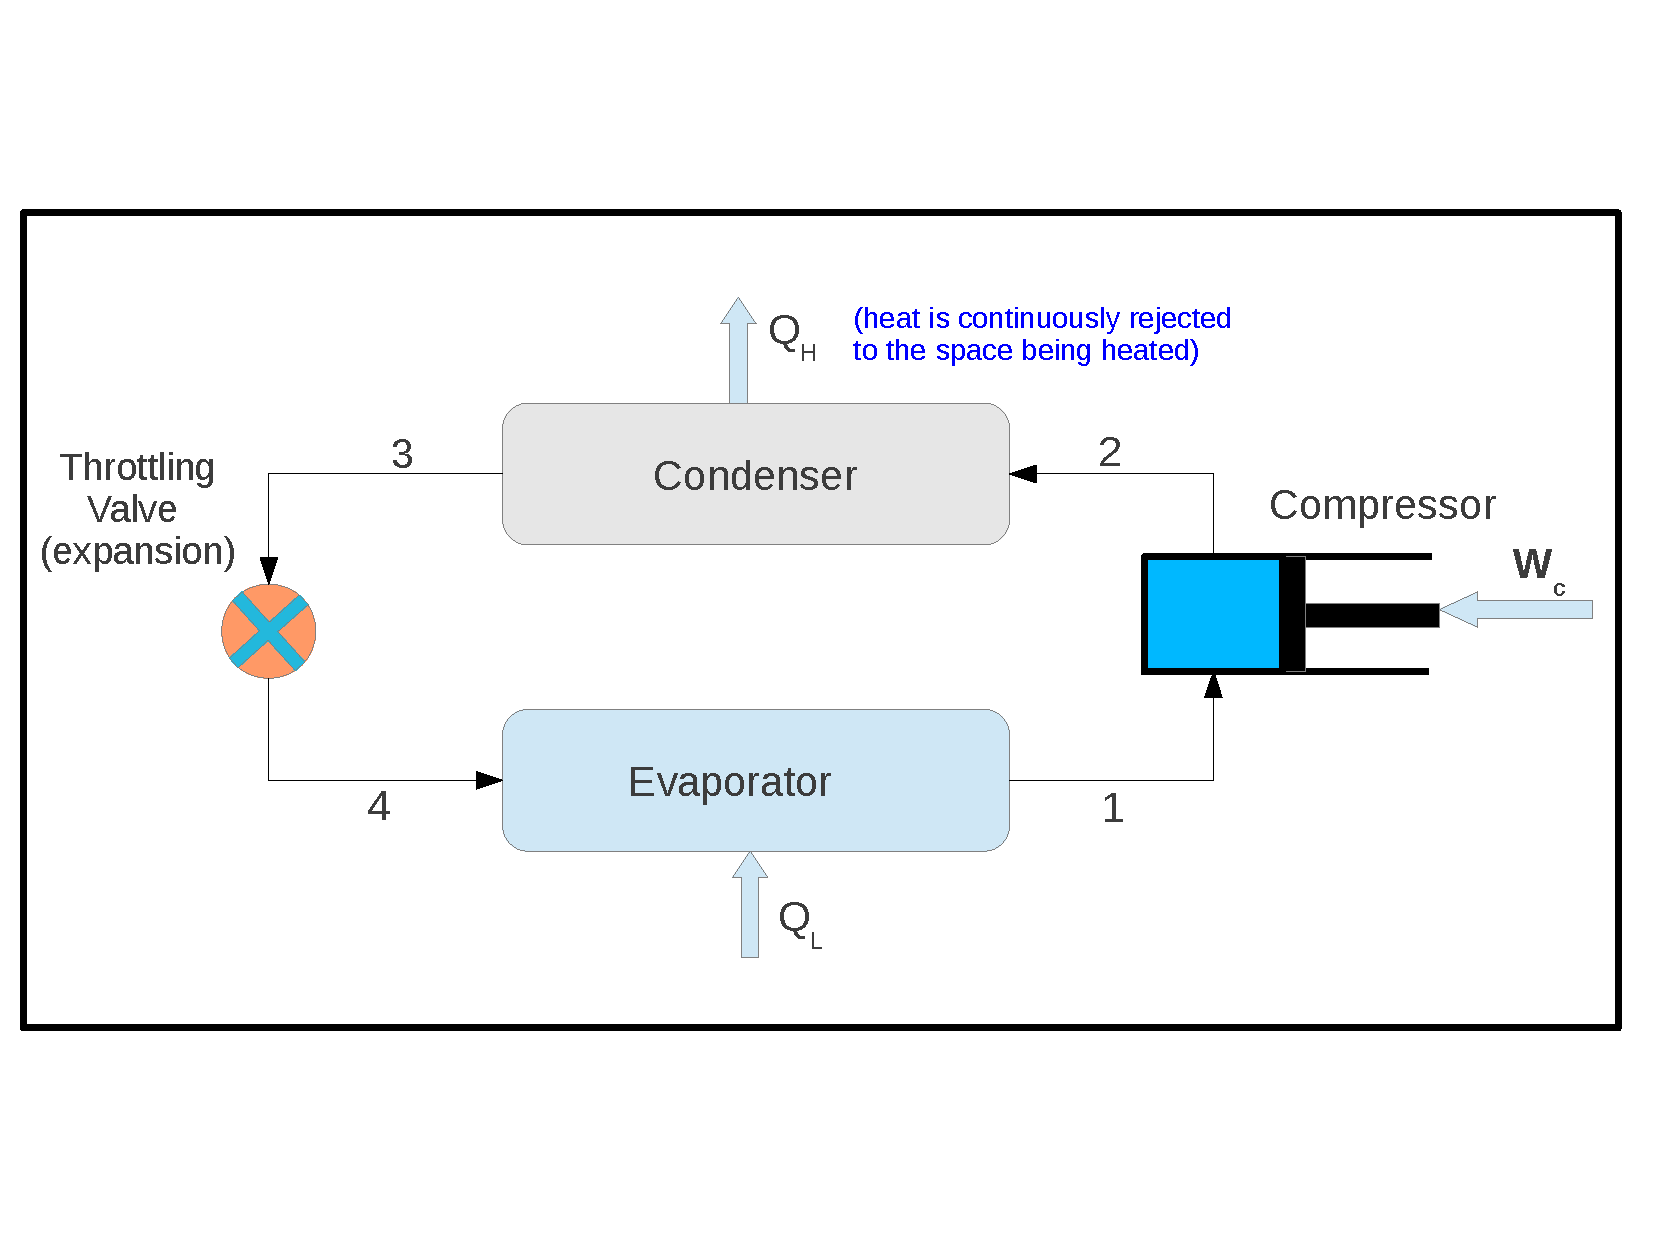
\includegraphics[width=4.5cm,clip]{./Pics/Overview_Refrig36}}
     \end{center}
    \end{figure}  
   \end{column}  
  \end{columns}
\end{frame}



%%%           %%%
%%%  SECTION  %%% 
%%%           %%%
\section{Summary}
%%%
%%% Slide
%%%
\begin{frame}
 \frametitle{Summary}
  \begin{itemize}
   \item <1-> Components of vapour power and refrigeration cycles;
   %\item <2-> Carnot cycle -- maximum possible efficiency derived from the Second Law of Thermodynamics;
   \item <3-> Rankine cycle is currently used in a number of industrial applications to transform thermal to mechanical/electrical energy;
   \item <4-> Practical improvements to the Rankine cycle to enhance thermal effciency.
   \item <5-> Components of refrigerant cycles;
   \item <6-> Coefficient of Performance;
   \item <7-> Refrigerants and Heat Pumps operate in the same way but with different objectives;
   \item <8-> The focal point in \textcolor{blue}{refrigerators} is the \textcolor{red}{heat absorbed from the Evaporator}, whereas;
   \item <9-> In \textcolor{blue}{heat pumps}, \textcolor{red}{heat is released in the Condenser}.
  \end{itemize}
\end{frame}


\end{document}
